\documentclass[aoas]{imsart}

\newcommand{\ba}{ {\boldsymbol a} }
\newcommand{\bA}{ {\boldsymbol A} }
\newcommand{\bb}{ {\boldsymbol b} }
\newcommand{\bB}{ {\boldsymbol B} }
\newcommand{\bc}{ {\boldsymbol c} }
\newcommand{\bC}{ {\boldsymbol C} }
\newcommand{\bd}{ {\boldsymbol d} }
\newcommand{\bD}{ {\boldsymbol D} }
\newcommand{\be}{ {\boldsymbol e} }
\newcommand{\bE}{ {\boldsymbol E} }
\newcommand{\boldf}{ {\boldsymbol f} }
\newcommand{\bF}{ {\boldsymbol F} }
\newcommand{\bg}{ {\boldsymbol g} }
\newcommand{\bG}{ {\boldsymbol G} }
\newcommand{\bh}{ {\boldsymbol h} }
\newcommand{\bH}{ {\boldsymbol H} }
\newcommand{\bi}{ {\boldsymbol i} }
\newcommand{\bI}{ {\boldsymbol I} }
\newcommand{\bj}{ {\boldsymbol j} }
\newcommand{\bJ}{ {\boldsymbol J} }
\newcommand{\bk}{ {\boldsymbol k} }
\newcommand{\bK}{ {\boldsymbol K} }
\newcommand{\bl}{ {\boldsymbol l} }
\newcommand{\bL}{ {\boldsymbol L} }
\newcommand{\bm}{ {\boldsymbol m} }
\newcommand{\bM}{ {\boldsymbol M} }
\newcommand{\bn}{ {\boldsymbol n} }
\newcommand{\bN}{ {\boldsymbol N} }
\newcommand{\bo}{ {\boldsymbol o} }
\newcommand{\bO}{ {\boldsymbol O} }
\newcommand{\bp}{ {\boldsymbol p} }
\newcommand{\bP}{ {\boldsymbol P} }
\newcommand{\bq}{ {\boldsymbol q} }
\newcommand{\bQ}{ {\boldsymbol Q} }
\newcommand{\br}{ {\boldsymbol r} }
\newcommand{\bR}{ {\boldsymbol R} }
\newcommand{\bs}{ {\boldsymbol s} }
\newcommand{\bS}{ {\boldsymbol S} }
\newcommand{\bt}{ {\boldsymbol t} }
\newcommand{\bT}{ {\boldsymbol T} }
\newcommand{\bu}{ {\boldsymbol u} }
\newcommand{\bU}{ {\boldsymbol U} }
\newcommand{\bv}{ {\boldsymbol v} }
\newcommand{\bV}{ {\boldsymbol V} }
\newcommand{\bw}{ {\boldsymbol w} }
\newcommand{\bW}{ {\boldsymbol W} }
\newcommand{\bx}{ {\boldsymbol x} }
\newcommand{\bX}{ {\boldsymbol X} }
\newcommand{\by}{ {\boldsymbol y} }
\newcommand{\bY}{ {\boldsymbol Y} }
\newcommand{\bz}{ {\boldsymbol z} }
\newcommand{\bZ}{ {\boldsymbol Z} }
\newcommand{\vc}[1]{\mbox{\boldmath $#1$}}
\newcommand{\balph}{ {\boldsymbol \alpha} }
\newcommand{\balpha}{ {\boldsymbol \alpha} }
\newcommand{\bbet}{ {\boldsymbol \beta} }
\newcommand{\bbeta}{ {\boldsymbol \beta} }
\newcommand{\bgam}{ {\boldsymbol \gamma} }
\newcommand{\bgamma}{ {\boldsymbol \gamma} }
\newcommand{\bGamma}{ {\boldsymbol \Gamma} }
\newcommand{\bdelta}{ {\boldsymbol \delta} }
\newcommand{\bDelta}{ {\boldsymbol \Delta} }
\newcommand{\beps}{ {\boldsymbol \epsilon} }
\newcommand{\bepsilon}{ {\boldsymbol \epsilon} }
\newcommand{\bphi}{ {\boldsymbol \phi} }
\newcommand{\bPhi}{ {\boldsymbol \Phi} }
\newcommand{\bpi}{ {\boldsymbol \pi} }
\newcommand{\bpsi}{ {\boldsymbol \psi} }
\newcommand{\bkap}{ {\boldsymbol \kappa} }
\newcommand{\bkappa}{ {\boldsymbol \kappa} }
\newcommand{\bKappa}{ {\boldsymbol \Kappa} }
\newcommand{\blam}{ {\boldsymbol \lambda} }
\newcommand{\blambda}{ {\boldsymbol \lambda} }
\newcommand{\bLambda}{ {\boldsymbol \Lambda} }
\newcommand{\bmu}{ {\boldsymbol \mu} }
\newcommand{\bMu}{ {\boldsymbol \Mu} }
\newcommand{\bet}{ {\boldsymbol \eta} }
\newcommand{\bome}{ {\boldsymbol \omega} }
\newcommand{\bomega}{ {\boldsymbol \omega} }
\newcommand{\bOmega}{ {\boldsymbol \Omega} }
\newcommand{\bnabla}{ {\boldsymbol \nabla} }
\newcommand{\brho}{ {\boldsymbol \rho} }
\newcommand{\bsigma}{ {\boldsymbol \sigma} }
\newcommand{\bSig}{ {\boldsymbol \Sigma} }
\newcommand{\bSigma}{ {\boldsymbol \Sigma} }
\newcommand{\btheta}{ {\boldsymbol \theta} }
\newcommand{\bTheta}{ {\boldsymbol \Theta} }
\newcommand{\bzeta}{ {\boldsymbol \zeta} }
\newcommand{\bPsi}{ {\boldsymbol \Psi} }
\newcommand{\btau}{ {\boldsymbol \tau} }
\newcommand{\bxi}{ {\boldsymbol \xi} }
\newcommand{\bzero}{ {\boldsymbol 0} }
\newcommand{\bones}{ {\boldsymbol 1} }
\newcommand{\given}{\,|\,}
\newcommand{\sS}{{\cal S}}
\newcommand{\Ss}{{\cal S}}
\newcommand{\Field}{{\cal F}}
\newcommand{\colsp}{{\cal C}}
\newcommand{\nullsp}{{\cal N}}
\newcommand{\rowsp}{{\cal R}}
\newcommand{\tildeC}{\tilde{C}}
\newcommand{\tildeK}{\tilde{K}}
\newcommand{\tildew}{\tilde{w}}
\newcommand{\tildebw}{\tilde{\bw}}
\newcommand{\tildebW}{\tilde{\bW}}
\newcommand{\calC}{{\cal C}}
\newcommand{\calcbC}{{\bf {\cal C}}}

% Do not remove even for final version
\newcommand{\kcomment}[1]{{\color{blue}{\{KR: #1\}}}}
\newcommand{\kc}{\kcomment}


\usepackage{amsmath}
\usepackage{pstricks,pst-grad}
\usepackage{graphicx}
\usepackage{floatrow}
\usepackage[linesnumbered,ruled,vlined]{algorithm2e}
\floatsetup[table]{capposition=top}
\usepackage{subfigure}
\usepackage[utf8]{inputenc}
\usepackage{booktabs}                     % horizontal lines in tables
\usepackage{comment}

% == Enable text degree
\usepackage{textcomp}

\usepackage{amsthm,amsmath,natbib}
\RequirePackage[colorlinks,citecolor=blue,urlcolor=blue]{hyperref}

% == Trygve Test
\usepackage{color, colortbl}
\definecolor{Gray}{gray}{0.9}

% put your definitions there:
\startlocaldefs
\newcommand{\edcomment}[1]{{\color{green}{\{Editor: #1\}}}}
\newcommand{\frevcomment}[1]{{\color{blue}{\{Rev 1: #1\}}}}
\newcommand{\srevcomment}[1]{{\color{red}{\{Rev 2: #1\}}}}
\newcommand{\trevcomment}[1]{{\color{violet}{\{Rev 3: #1\}}}}
\endlocaldefs

% New Marcos.
\usepackage{amssymb}
\usepackage{hyperref}
\usepackage{cleveref}
% For testing whether an argument of a macro is empty.
\usepackage{xifthen}
\usepackage{bm}
\usepackage{bbm}

\newcommand{\dl}{\mathrm{d}\lambda}
\newcommand{\R}{\mathbb{R}}
\newcommand{\x}{s}
\newcommand{\uu}{u}
\newcommand{\vv}{v}
%\newcommand{\bt}{t}
\newcommand{\T}{T}
\newcommand{\es}{\Gamma}%\mathrm{ES}}
\newcommand{\ibv}{\mathrm{IBV}}
\newcommand{\emv}{\mathrm{EMV}}
\newcommand{\eibv}{\mathrm{EIBV}}
\newcommand{\eemv}{\mathrm{EEMV}}
\newcommand{\mes}{\nu}
% \newcommand{\gp}{\xi}
\newcommand{\no}{p}
\newcommand{\eps}{\varepsilon}
\newcommand{\sigeps}{\Sigma_{\eps}}
\newcommand{\cov}{\operatorname{Cov}}
\newcommand{\norm}{\mathcal{N}}
\newtheorem{propo}{Proposition}
\newtheorem{theorem}{Theorem}
\newtheorem{remark}{Remark}
\newtheorem*{remark*}{Remark}


\DeclareMathOperator*{\argmin}{\arg\!\min}

% Mean and cov at time zero.
\newcommand{\mean}[1]{\mu
\left(#1\right)}
\newcommand{\covmat}[1]{K
\left(#1\right)}

% Product measure.
\newcommand{\productMeasure}{
\mathrm{d}\nu^{\otimes}\left(\bm{u}\right)}

% Field value at x. Can either switch between parenthesis or subscripting.
% If no argument provided, then will just print xi.
\newcommand{\gp}[1][]{
    \ifthenelse{\isempty{#1}}
    {Z}
    {Z_{#1}}
}

% Misc. covariance matrices
\newcommand{\covV}{C_{V}}
\newcommand{\covN}{C}


% Covariance function k(., .).
\newcommand{\covFunc}[4]{k_{#2#4}\left(#1,#3\right)}

% Covariance matrix K = k(X, X).
\newcommand{\covMat}[4]{\bm{K}_{#2#4}(#1#3)}

% Mean function \mu(x).
\newcommand{\meanFunc}[2]{\mu_{#2}\left(#1\right)}

% Mean vector \mu(X).
\newcommand{\meanVec}[2]{\bm{\mu}_{#2}(#1)}

% Excursion probability in the set T^r.
\newcommand{\jointExcuProb}{
    \mathbb{P}\left(
    \gp[\bm{u}]\in T^r \right)
}

% In Proposition 1, the mean vector at the uu concatenation and the
% corresponding covariance matrix.
\newcommand{\meanUU}{
    \mu(\bm{u})
}

\newcommand{\covUU}{
    K\left(\bm{u},\bm{u}\right)
}

% ----------
% SEQUENTIAL
% ----------
% Probability distribution now (after 1 conditioning).
\newcommand{\currentProba}[1]{\mathbb{P}_{[n]}
\left(#1\right)}
% Probability distribution in the future (after 2 conditioning).
\newcommand{\futureProba}[1]{\mathbb{P}_{[n+1]}
\left(#1\right)}

% Same for expectations.
\newcommand{\currentExp}[1]{\mathbb{E}_{[n]}
\left[#1\right]}
\newcommand{\futureExp}[1]{\mathbb{E}_{[n+1]}
\left[#1\right]}

% For mean vectors.
\newcommand{\currentMean}[1]{\mu_{[n]}
\left(#1\right)}
\newcommand{\futureMean}[1]{\mu_{[n+1]}
\left(#1\right)}

% And covariance matrices.
\newcommand{\currentCov}[1]{K_{[n]}
\left(#1\right)}
\newcommand{\futureCov}[1]{K_{[n+1]}
\left(#1\right)}


% For nice expectations.
\usepackage{mathtools}
\newcommand{\expect}{\mathbb{E}\expectarg}
\DeclarePairedDelimiterX{\expectarg}[1]{[}{]}{%
  \ifnum\currentgrouptype=16 \else\begingroup\fi
  \activatebar#1
  \ifnum\currentgrouptype=16 \else\endgroup\fi
}

\newcommand{\innermid}{\nonscript\;\delimsize\vert\nonscript\;}
\newcommand{\activatebar}{%
  \begingroup\lccode`\~=`\|
  \lowercase{\endgroup\let~}\innermid
  \mathcode`|=\string"8000
}


\begin{document}

\begin{frontmatter}

% "New Title of the paper"
\title{Autonomous Oceanographic Data Collection towards Estimating Excursion Sets of Vector-valued Random Fields} 
\runtitle{Autonomous Oceanographic Data Collection}

% "Former Title of the paper" (DG 08.06.2020)
%\title{Autonomous Oceanographic Sampling Designs using Excursion Sets for Multivariate Gaussian random fields} \runtitle{Excursion Probabilities for Informative Sampling}

\begin{aug}
\author{\fnms{Trygve Olav} \snm{Fossum}\thanksref{t1,t2}, \corref{} \ead[label=e1]{trygve.o.fossum@ntnu.no}}
\author{\fnms{Cédric} \snm{Travelletti}\thanksref{t3}, \corref{} \ead[label=e2]{cedric.travelletti@stat.unibe.ch}}
\author{\fnms{Jo} \snm{Eidsvik}\thanksref{t4}, \ead[label=e3]{jo.eidsvik@ntnu.no}}
\author{\fnms{David} \snm{Ginsbourger}\thanksref{t3}, \ead[label=e4]{david.ginsbourger@stat.unibe.ch}}
\and
\author{\fnms{Kanna} \snm{Rajan}\thanksref{t5}. \ead[label=e5]{kanna.rajan@fe.up.pt}}

\affiliation[t1]{Department of Marine Technology, The Norwegian University of Science and Technology (NTNU), Trondheim, Norway.} 
\affiliation[t2]{Centre for Autonomous Marine Operations and Systems, NTNU.}
\affiliation[t3]{Institute of Mathematical Statistics and Actuarial Science, University of Bern, Switzerland.}
\affiliation[t4]{Department of Mathematical Sciences, NTNU.}
\affiliation[t5]{Underwater Systems and Technology Laboratory, Faculty of Engineering, University of Porto, Portugal.}

\address{\\Trygve Olav Fossum \\Department of Marine Technology\\ Otto Nielsens veg. 10, 7491 Trondheim\\ Norway\\
\printead{e1}}
\address{Cédric Travelletti\\ Institute of Mathematical Statistics and Actuarial Science \\ University of Bern \\
Switzerland.
\printead{e2}}
\address{Jo Eidsvik\\Department of Mathematical Sciences\\ Hogskoleringen 1, 7491 Trondheim\\ Norway\\ \printead{e3}}
\address{David Ginsbourger\\ Institute of Mathematical Statistics and Actuarial Science \\ University of Bern \\
Switzerland.
\printead{e4}}
\address{Kanna Rajan\\Underwater Systems and Technology Laboratory,
  Faculty of Engineering,\\ Rua Dr. Roberto Frias\\ University of Porto, Portugal\\
\printead{e5}}

\runauthor{TO. Fossum et al.}
\end{aug}

\begin{abstract}

  Improving and optimizing oceanographic sampling is a crucial task
  for marine science and maritime management. Faced with limited
  resources to understand processes in the water-column, the
  combination of statistics and autonomous robotics provides new
  opportunities for experimental design. In this work we develop
  methods for efficient spatial sampling applied to the mapping of
  coastal ocean processes by providing informative descriptions of
  spatial characteristics of ocean phenomena. Specifically, we define
  a design
  criterion based on improved characterization of the uncertainty in
  the excursions of vector-valued Gaussian random fields, and derive
  tractable expressions for the expected Bernoulli variance reduction
  in such a framework. We demonstrate how this criterion can be used
  to prioritize sampling efforts at locations that are ambiguous,
  making exploration more effective. We use simulations to study the
  properties of methods and to compare them with state-of-the-art
  approaches, followed by results from field deployments with an
  autonomous underwater vehicle (AUV) as part of a study mapping the
  boundary of a river plume. The results demonstrate the potential of
  combining statistical methods and robotic platforms to effectively
  inform and execute data-driven environmental sampling.
  
%Motivated by the challenges related to efficient allocation of sampling resources in environmental sensing, the combination of Excursion Probabilities and Gaussian process modeling is explored for autonomous robotic sampling of ocean features; enabling information driven measures  sampling efforts to high-interest regions. These regions are usually characterized by gradients of measurable environmental variables, e.g., temperature or salinity gradients, on which EPs subsequently can be used...Correlation among samples and multivariate requirements are typical in environmental studies.

\end{abstract}

\begin{keyword}
\kwd{Ocean Sampling}
\kwd{Excursion Sets}
\kwd{Gaussian Processes}
\kwd{Experimental Design}
\kwd{Autonomous robots}
\kwd{Adaptive Information Gathering}
\end{keyword}

\end{frontmatter}
\section{Introduction}

%NB: The subsections are used as a temporary instrument to highlight the proposed structure and should probably be abolished upon convergence to a stable version.

\subsection{Oceanic data collection and spatial design of experiments}

%\textcolor{blue}{NB: I started to match previously listed thoughts/ideas with pieces of the former intro. Will do more asap. Also, Section 3 I find excellent (and more precise than the intro) and start thinking that some bits might end up in the newer intro (while some others could land in a later section).}


Monitoring the world's oceans has gained increased importance in light of the changing climate and increasing anthropogenic impact. 
\begin{comment} % TO BE RE-INSERTED LATER IN THE ETXT?
A central problem for understanding these factors is the lack of representative data with sufficient resolution. Most of this \emph{undersampling} can be attributed to the large spatio-temporal variations in which ocean processes transpire, prompting the need for effective means of sampling. By \emph{sampling}, we refer to the design of observational strategies in the spatial domain, where the use autonomous robotic platforms can be combined with statistical methods to pursue measurements with high scientific relevance. This combination, of statistical tools and robotic platforms, constitute a methodological basis for addressing the problem of efficient sampling of the ocean, which is at the core of this work.
\end{comment}
Central to understanding the changes taking place in the upper
water-column is knowledge of the bio-geophysical interaction driven by
an agglomeration of physical forcings (e.g. wind, topography,
bathymetry, tidal influences, etc.) and incipient micro-biology driven
by planktonic and coastal anthropogenic input, such as pollution and
agricultural runoff transported into the ocean by rivers and streams.
These often result in a range of ecosystem-related phenomena such as
blooms and plumes, with direct and indirect effects on society. \kc{we
  should look for a citation here. Check with John Ryan}
 One of the bottlenecks in the study of such phenomena lies however in the lack of obervational data with sufficient resolution. Most of this \emph{undersampling} can be attributed to the large spatio-temporal variations in which ocean processes transpire, prompting the need for effective means of data collection. Based on collected data and sometimes also of prior knowledge, models from spatial statistics can be used to make predictions of the state variables under consideration over regions of interest. In case of multiple continuous state variables being jointly studied relying on spatially scattered data, vector-valued random field models and associated prediction approaches such as co-Kriging (REFs) can be considered nowadays as part of the standard statistical toolkit in oceanographic research and beyond. %applications and beyond.  
 %By \emph{sampling}, we refer to the design of observational strategies in the spatial domain, where the use autonomous robotic platforms can be combined with statistical methods to pursue measurements with high scientific relevance. This combination, of statistical tools and robotic platforms, constitute a methodological basis for addressing the problem of efficient sampling of the ocean, which is at the core of this work.
  


Traditional data collection to understand natural and artificial phenomena at sea has typically been based on static buoys, floats, or ship-based methods,
with significant logistical limitations that directly impact coverage
and sampling resolution. Modern methods using satellite remote-sensing
provide large-scale coverage but have limited resolution, are limited
to sensing the surface, and are impacted by cloud cover. Numerical
ocean models similarly find it challenging to provide detail at fine
scale \citep{Lermusiaux:2006}, and also come with computation costs that can be practically limiting. 
%limiting computing resources, no time for hard-core ocean model Navier-Stokes, hence GPs and approximations, etc.
%
\begin{figure}[!h] 
  \centering 
  \subfigure[Illustration of an ocean sensing network and the sense-plan-act control methodology.]{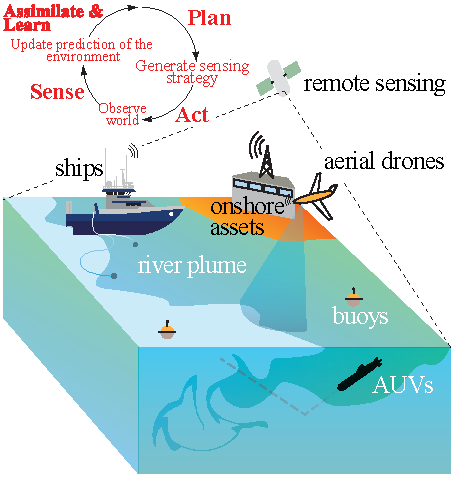
\includegraphics[width =
    0.49\textwidth]{Figures/envir2.pdf}\label{fig:envir1}}
  \hfill
  \subfigure[Frontal patterns off of the Nidelva river, Trondheim, Norway.]{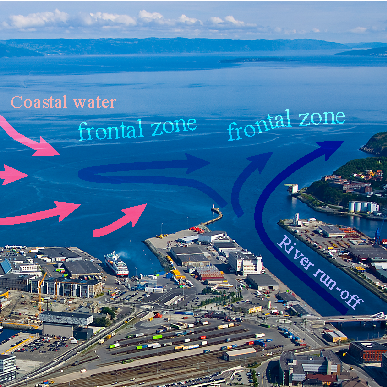
\includegraphics[width =
    0.49\textwidth]{Figures/river_proccess.pdf}\label{fig:nidelven}}
  \caption{\ref{fig:envir1} Traditional ocean observation based on 
    ship-based sampling has been augmented by autonomous
    robotic vehicles. % and their interactions.  
    AUV platforms are an integral part of this network being able to
    reason and make decisions for efficient onboard adaptive sampling.
    % using the sense-plan-act control approach to autonomous control. 
    \ref{fig:nidelven} The interaction of river and ocean creates
    processes that are challenging to map, where the combination of
    statistics and robotics can play a vital role in enabling more
    effective oceanographic observation.\kc{The inset ``AUV robot''
      looks very tacky and ad-hoc; might be best to remove it. Change
      ``ships'' to
      ``Ship'', remove the aerial drone, since we didn't use it and
      don't plan to in this work.}}
  \label{fig:envir} \end{figure}
%
\begin{comment} % Somehow redundant with the parag following below
Mobile robotic platforms \citep{Bellingham07} have contributed significantly to environmental monitoring and sampling. In particular, AUVs have advanced the state of in-situ sampling, and made robotics an integral part of ocean observation, filling parts of the undersampling gap \cite{rudnick03,rudnick18} (See Fig. \ref{fig:envir1}).
\end{comment}
%
The advent of robust mobile robotic platforms \citep{Bellingham07} has
resulted in significant contributions to environmental monitoring and
sampling in the ocean. In particular, autonomous underwater vehicles (AUVs) have advanced the state of data collection and consequently have made robotics an integral part of ocean observation; %our 
previous work by some of the authors of the present paper have contributed to this effort \citep{das11b,Das2015,fossuminformation,fossum18b}. 


As full numerical ocean models based on complex differential equations cannot be run onboard a marine robot with limited computational capacity, statistical models relying on collected data and random field assumptions appear quite relevant as means to guide AUV data collection trajectories. Our main research angle in the present work is to extend sequential design strategies from the world of spatial statistics and computer experiments to frameworks featuring both vector-valued observational data and experimental designs that may be constrained by the nature of measurement paths.      
\\

Surveys with AUVs are usually limited to observations along fixed
transects that are pre-scripted in mission plans created manually by a
human operator. Missions can be specified operating on a scale of
hundreds of meters to tens of kilometers depending on the scientific
context. Faced with limited coverage capacity, a more effective
approach is to instead use onboard algorithms to continuously
evaluate, update, and refine future sampling locations (sense-plan-act
cycle in Fig. \ref{fig:envir1}), making the information gathering
\emph{adaptive} \citep{das11b,Das2015,fossuminformation,fossum18b}.
% This usually occurs on a spatial grid, called a waypoint graph. 
In doing so, the space of sampling opportunities is still limited by
the so-called waypoint graph, a discretization of the search domain, but the AUV has flexibility to modify its path at each waypoint based on in-situ sensing and measurements onboard \citep{py10,Rajan12,Rajan12b}.\\

The work presented here is primarily inspired by a cast study 
%application where an AUV is used to measure both temperature and salinity in 
pertaining to the spatial characterization of a frontal system generated by
river plumes. Fig. \ref{fig:nidelven} shows the survey area in
Trondheim, Norway, where cold freshwater enters from the river,
creating a strong gradient in both temperature and salinity. Because
of the local topography and the Coriolis force the cold fresh water
tends to flow to the east. Depending on the river discharge, tidal
effects, wind, and temperature differences, this boundary often gets
distorted. Initial knowledge about the location and evolution of these
features are highly uncertain, making deterministic planning
challenging. Here the goal is to use AUV measurements towards a better identification of freshwater versus oceanic water, with the help of a vector-valued random field model for both temperature and salinity. As we will present in the next sections, some of the original contributions inspired by this specific problem are actually applicable to further settings and application areas. \\

The questions tackled here hence pertain to the broader area of spatial data collection and experimental design, yet with the particularity of estimating some regions of the domain, mostly excursion sets, being implicitly defined by a scarcely observed vector-valued random field. 
%because of limited resources to sample the large oceanographic domains, one must plan for active learning during the operation, where a relevant criterion is used to extract the most valuable designs. The acquired in-situ information must then be assimilated into the statistical model onboard the platform, so that it can be used to re-compute the sampling criterion and in this way inform decisions on where to sample next. \\
Moreover, given constraints on AUV movements and the fact that surveya rely by design in such a framework on successive measurements spread along a trajectory, addressing corresponding design problems calls for particular sequential strategies, possibly also accounting for the finiteness of resources by anticipating multiple steps ahead thereby improving over myopic strategies. \\

Here we aim to leverage and extent recent progress in uncertainty quantification and reduction for excursion sets of Gaussian random fields in order to address vector-valued observational cases under constrained design such as in the motivating application of designing AUV trajectories to better distinguish between freshwater from ocean waters by relying on temperature and salinity measurements. %approach will take substantial advantage of existing work in the field of excursion set estimation mainly dedicated to computer experiments in the scalar-valued case, and where space exploration can be performed without constraints regarding the distance between successive design points. 
Original contributions compared to recent related work in the framework of scalar-valued computer experiments include: 
\begin{itemize}
    \item Extension of two important Sequential Uncertainty Reduction criteria of (REFs) to homotopic or heterotopic vector-valued settings,
    \item Investigation of myopic and multiple-step ahead batch-sequential strategies for optimizing trajectories with respect to such criteria,
    \item Replicable experiments with synthetic test cases and original data sets with accompagnying codes 
\end{itemize}
Let us briefly review random field modelling and recent advances in targetd sequential design of experiments based on Gaussian Processes before detailing further existing literature tackling the considered problems, our proposed approach, as well as outlining the rest of the paper.  


\subsection{Random field modelling and targeted sequential design of experiments}

\begin{itemize}
    \item 
\end{itemize}

% From earlier version; to be relocated?
%Hence statistical proxy models of the environment must be used. For our purpose, we rely on Gaussian process (GP) representations of the ocean variables of interest because they are computationally convenient and yet provide enough flexibility to realistically model the spatial variability and dependence, and the correlation between multiple processes. 
\subsection{Related work and proposed approach in a nutshell}

\begin{itemize}
    \item 
\end{itemize}

\textcolor{blue}{We might want to re-use some of the following (from earlier version):}

A major contribution of our work is to derive closed-form results for
this design criteria for situations where the underlying model is
based on multivariate GPs. Another contribution is that we embed this
approach in a sequential strategy to produce sampling algorithms, and
apply this to a real-world scenario of autonomously sampling
temperature and salinity gradients using an AUV, with the intention of
characterizing the variability of oceanic and riverine waters in
typical mixed coastal environments.

Motivating examples relevant for ESs of multivariate processes are
abundant. In medicine, doctors do not rely solely on a single symptom
but must see several combined effects before making a diagnosis. In
our context of environmental sampling, the salinity and temperature
excursions of a river plume can similarly help characterize the
underlying bio-geochemical processes
\citep{hopkins2013detection,Pinto2018}, where sampling can be aimed
towards reducing uncertainty in the temperature and salinity ES.
Unlike what has been done in previous plume exploration studies, we
emphasize the links to spatial statistical modeling and targeted
multivariate sampling criteria for sequential sampling.

Other statistical
work in the oceanographic domain include \cite{wikle2013modern}
focusing on hierarchical statistical models; \cite{sahu2008space},
studying spatio-temporal models for sea surface temperature and
salinity data; and \cite{mellucci2018oceanic} looking at the
statistical prediction of features using an underwater glider.
In this paper the focus is not on statistical modeling, but rather on statistical results and computations for efficient sampling designs. 

We focus on spatial characterization of a frontal system generated by
river plumes. Fig. \ref{fig:nidelven} shows the survey area in
Trondheim, Norway, where cold freshwater enters from the river,
creating a strong gradient in both temperature and salinity. Because
of the local topography and the Coriolis force the cold fresh water
tends to flow to the east. Depending on the river discharge, tidal
effects, wind, and temperature differences, this boundary often gets
distorted. Initial knowledge about the location and evolution of these
features are highly uncertain, making deterministic planning
challenging.

Adaptive in-situ AUV sampling of an evolving frontal feature has been
explored in \cite{fronts11,Zhang2012,Pinto2018,costa19}. These
approaches typically use a reactive-adaptive scheme, whereby
exploration does not rely on a statistical model of the environment,
but rather adaptation is based on closing the sensing and actuation
loop. Myopic sampling, i.e. stage-wise selection of the path (on the
waypoint graph), has been used for surveys
\citep{singh2009efficient,Binney2013} that focus largely on reducing
predictive variance or entropy. These criteria are widely adopted in
the statistics literature on spatio-temporal design as well
\cite{bueso1998state,zidek2019monitoring}, but variance and entropy
reduction are independent of the actual data realizations under the
assumptions of GP models, so it has limited
decisional flexibility. The use of data-driven adaptive criteria
was introduced to include more targeted sampling of regions of
scientific interest in \cite{Low2009} and \cite{fossuminformation}. In
this paper, we focus on mapping the river plume by rewarding designs
that improve the classification of ES in temperature and salinity.


\subsection{Outline of the paper and its appendices / supplemental material}

\begin{itemize}
    \item 
\end{itemize}

The remainder of this paper is organized as follows: 
%Section \ref{sec:bg} provides select background on ocean sampling. 
Section \ref{sec:ESEP} defines ESs, EPs, and the design criteria of IBV for
vector-valued GPs. Section \ref{sec:heuristics} builds on these
assumptions when deriving the sequential design criteria for adaptive
sampling. Section \ref{sec:simulations} discusses properties of the
methods in simulation studies. Section \ref{sec:case_study}
demonstrates the methodology used in field work characterizing a river
plume and finally, Section \ref{sec:concl_disc} contains a summary and
a discussion of future work.

%\subsection{}

%\begin{itemize}
%    \item 
%\end{itemize}

\begin{comment}
\section{Former Introduction (Before 08.06.2020)}

Monitoring the world's oceans has gained increased importance in light
of the changing climate and increasing anthropogenic impact. 
A central problem for understanding these factors is the lack of representative data with sufficient resolution. Most of this \emph{undersampling} can be attributed to the large spatio-temporal variations in which ocean processes transpire, prompting the need for effective means of sampling. By \emph{sampling}, we refer to the design of observational strategies in the spatial domain, where the use autonomous robotic platforms can be combined with statistical methods to pursue measurements with high scientific relevance. This combination, of statistical tools and robotic platforms, constitute a methodological basis for addressing the problem of efficient sampling of the ocean, which is at the core of this work.

The
advent of robust mobile robotic platforms \citep{Bellingham07} has
resulted in significant contributions to environmental monitoring and
sampling in the ocean. In particular, autonomous underwater vehicles (AUVs), have
advanced the state of sampling and consequently have made robotics an
integral part of ocean observation; our previous work has contributed
to this effort \citep{das11b,Das2015,fossuminformation,fossum18b}. 

The potential that lies in using information-based sampling methods, which we
highlight in this paper, is to do efficient environmental sampling and
overcome common challenges as discussed next. First, full numerical ocean models based on complex
differential equations cannot be run onboard a marine robot with
limited computational capacity.
% provide accurate results for online
% operations because the onboard computers lack the computational power
% required.
Hence statistical proxy models of the environment must be used. For our purpose, we rely on Gaussian process (GP)
representations of the ocean variables of interest because they are computationally convenient and yet provide enough flexibility to realistically model the spatial variability and dependence, and the correlation between multiple processes. Second, because of limited resources to sample the large oceanographic domains, one must plan for
active learning during the operation, where a relevant criterion is
used to extract the most valuable designs. The acquired in-situ
information must then be assimilated into the statistical model
onboard the platform, so that it can be used to re-compute the
sampling criterion and in this way inform decisions on where to sample
next. We use a criterion focusing on the prediction of excursion sets
(ESs) for the multivariate spatial processes of interest. Third, the
number of sampling designs is enormous, creating a trade-off between
optimization and computability. One must often compromise in both
development and practical operations, and we will rely on
short-horizon optimization routines for sequential designs among
nearest neighbors points in a spatial grid (waypoint graph).

\kc{The para above needs a rewrite to me. It starts off by stating
  there are challenges. But then jumps to models without stating the
  connection with sampling, and then jumps into learning without
  stating why learning is important. Typically the English in formal
  text starts with a statement which is supported or clarified. In the
  two cases above, the connections are simply not obvious. If this was
  there in the first version of the m/s submitted, I'm not sure why
  the reviewers didn't catch it. This is not just a stylistic issue;
  it has to do with making sense and bring the reader/reviewer along.}

\kc{Second, I don't see a motivation for GPs here and as I read
  further into the text. Even for stats folks, are GPs the ``best''
  ways to go? Are they obviously the tools one would use in
  environmental sampling? And even if they are, I think we ought to
  make the case for it strongly and generally, so this paper is
  actually accessible and understandable to those not in the Spatial
  Stats field. I would suggest adding a short para on GPs and why
  they're important -- i.e. motivate the use of GPs early, so we can
  freely make attributions to them later, as in the next section, for
  example.} 

The imperfect understanding of causality coupled with the underlying
fundamental uncertainty of the ocean implies that we need to make a
large number of measurements. In addition, the use statistical models
and methods to determine what and how phenomena form, is one way to
increase the quality of predictive power aiding our understanding of
upper water-column processes. 

With this in mind, we design AUV sampling strategies for reducing the spatially-integrated Bernoulli variance (IBV) in the ES
indicator variables. 
ES of random fields are thoroughly presented in \citep{adler2009random}. Recent work on ESs and associated excursion
probabilities (EPs) connected to spatial statistics include
\cite{french2013spatio,bolin2015excursion,french2016credible}. Our
focus is on uncertainty characterization and how this is influenced by
sampling. In this sense, our work is similar to
\cite{bect2012,chevalier2014fast,azzimonti2016quantifying} who
describe analytical results for the IBV for univariate processes.

A major contribution of our work is to derive closed-form results for
this design criteria for situations where the underlying model is
based on multivariate GPs. Another contribution is that we embed this
approach in a sequential strategy to produce sampling algorithms, and
apply this to a real-world scenario of autonomously sampling
temperature and salinity gradients using an AUV, with the intention of
characterizing the variability of oceanic and riverine waters in
typical mixed coastal environments.

Motivating examples relevant for ESs of multivariate processes are
abundant. In medicine, doctors do not rely solely on a single symptom
but must see several combined effects before making a diagnosis. In
our context of environmental sampling, the salinity and temperature
excursions of a river plume can similarly help characterize the
underlying bio-geochemical processes
\citep{hopkins2013detection,Pinto2018}, where sampling can be aimed
towards reducing uncertainty in the temperature and salinity ES.
Unlike what has been done in previous plume exploration studies, we
emphasize the links to spatial statistical modeling and targeted
multivariate sampling criteria for sequential sampling.

Other statistical
work in the oceanographic domain include \cite{wikle2013modern}
focusing on hierarchical statistical models; \cite{sahu2008space},
studying spatio-temporal models for sea surface temperature and
salinity data; and \cite{mellucci2018oceanic} looking at the
statistical prediction of features using an underwater glider.
In this paper the focus is not on statistical modeling, but rather on statistical results and computations for efficient sampling designs. 

The remainder of this paper is organized as follows: Section
\ref{sec:bg} provides select background on ocean sampling. Section
\ref{sec:ESEP} defines ESs, EPs, and the design criteria of IBV for
vector-valued GPs. Section \ref{sec:heuristics} builds on these
assumptions when deriving the sequential design criteria for adaptive
sampling. Section \ref{sec:simulations} discusses properties of the
methods in simulation studies. Section \ref{sec:case_study}
demonstrates the methodology used in field work characterizing a river
plume and finally, Section \ref{sec:concl_disc} contains a summary and
a discussion of future work.
\end{comment}

\begin{comment}
\section{Ocean Processes and Observation}
\label{sec:bg}

Central to understanding the changes taking place in the upper
water-column is knowledge of the bio-geophysical interaction driven by
an agglomeration of physical forcings (e.g. wind, topography,
bathymetry, tidal influences, etc.) and incipient micro-biology driven
by planktonic and coastal anthropogenic input, such as pollution and
agricultural runoff transported into the ocean by rivers and streams.
These often result in a range of ecosystem-related phenomena such as
blooms and plumes, with direct and indirect effects on society. \kc{we
  should look for a citation here. Check with John Ryan}

Traditional data collection to understand such phenomena at sea has
typically been based on static buoys, floats, or ship-based methods,
with significant logistical limitations that directly impact coverage
and sampling resolution. Modern methods using satellite remote-sensing
provide large-scale coverage but have limited resolution, are limited
to sensing the surface, and are impacted by cloud cover. Numerical
ocean models similarly find it challenging to provide detail at fine
scale \citep{Lermusiaux:2006}. Mobile robotic platforms
\citep{Bellingham07} have contributed significantly to environmental monitoring and sampling. In particular, AUVs have
advanced the state of in-situ sampling, and made robotics an integral
part of ocean observation, filling parts of the undersampling gap
\cite{rudnick03,rudnick18}(See Fig. \ref{fig:envir1}).

%Walter Munk referred to the 20\textsuperscript{th} century
%as the \emph{century of undersampling} \citep{munk2002}, pointing out
%a lack of sufficient sampling resolution in time and space as a
%critical issue for characterizing ocean phenomena. Even today,
%policymakers struggle with limited observability of severe
%environmental problems; a prominent example is the recent (May 2018)
%outbreak of harmful algal blooms in Northern Norway\footnote{Report
%  from the Institute of Marine Research: https://bit.ly/2KZGJfI}, with
%losses exceeding 12 million tons of salmon valued at \$80 million
%(Norwegian Directorate of Fisheries). This is a case in point of how
%adequate sampling efforts could have provided a more accurate
%assessment and early warning of changing environmental conditions.

\begin{figure}[!h] 
  \centering 
  \subfigure[Illustration of an ocean sensing network and the sense-plan-act control methodology.]{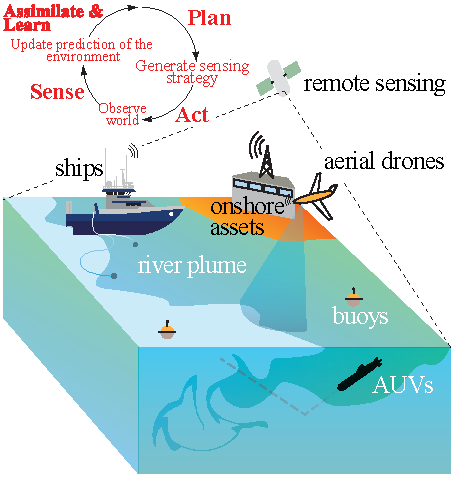
\includegraphics[width =
    0.49\textwidth]{Figures/envir2.pdf}\label{fig:envir1}}
  \hfill
  \subfigure[Frontal patterns off of the Nidelva river, Trondheim, Norway.]{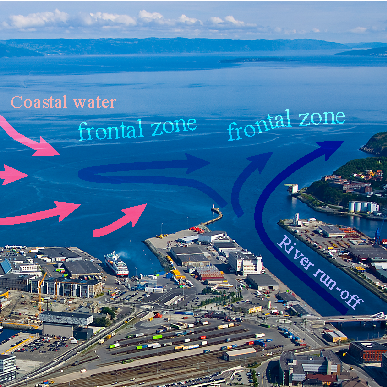
\includegraphics[width =
    0.49\textwidth]{Figures/river_proccess.pdf}\label{fig:nidelven}}
  \caption{\ref{fig:envir1} Traditional ocean observation based on 
    ship-based sampling has been augmented by autonomous
    robotic vehicles. % and their interactions.  
    AUV platforms are an integral part of this network being able to
    reason and make decisions for efficient onboard adaptive sampling.
    % using the sense-plan-act control approach to autonomous control. 
    \ref{fig:nidelven} The interaction of river and ocean creates
    processes that are challenging to map, where the combination of
    statistics and robotics can play a vital role in enabling more
    effective oceanographic observation.\kc{The inset ``AUV robot''
      looks very tacky and ad-hoc; might be best to remove it. Change
      ``ships'' to
      ``Ship'', remove the aerial drone, since we didn't use it and
      don't plan to in this work.}}
  \label{fig:envir} \end{figure}

\end{comment}

\subsection{To be relocated elsewhere}
The AUVs considered here are powered untethered platforms, that
operate at $1$-$3$ m/s in the upper water column, where they are free
to move in six degrees of freedom (6 DOF). The in-water operation time
capability depends on survey speed, payload sensors and navigation;
typically this amounts to 8-48 hrs. AUVs typically use single-board
computers (SBCs), like the Raspberry Pi or a multicore GPU NVIDIA
Jetson TX1 (quad-core 1.91 GHz 64-bit ARM machine, a 2-MB L2 shared
cache, and 4 GB of 1600 MHz DRAM) for computation onboard.

\begin{comment}
Surveys with AUVs are usually limited to observations along fixed
transects that are pre-scripted in mission plans created manually by a
human operator. The mission can be specified operating on a scale of
hundreds of meters to tens of kilometers depending on the scientific
context. Faced with limited coverage capacity, a more effective
approach is to instead use onboard algorithms to continuously
evaluate, update, and refine future sampling locations (sense-plan-act
cycle in Fig. \ref{fig:envir1}), making the information gathering
\emph{adaptive} \citep{das11b,Das2015,fossuminformation,fossum18b}.
% This usually occurs on a spatial grid, called a waypoint graph. 
In doing so, the space of sampling opportunities is still limited by
the waypoint graph, but the AUV has flexibility to modify its path at
each waypoint based on in-situ sensing and measurements onboard
\citep{py10,Rajan12,Rajan12b}.


We focus on spatial characterization of a frontal system generated by
river plumes. Fig. \ref{fig:nidelven} shows the survey area in
Trondheim, Norway, where cold freshwater enters from the river,
creating a strong gradient in both temperature and salinity. Because
of the local topography and the Coriolis force the cold fresh water
tends to flow to the east. Depending on the river discharge, tidal
effects, wind, and temperature differences, this boundary often gets
distorted. Initial knowledge about the location and evolution of these
features are highly uncertain, making deterministic planning
challenging.

Adaptive in-situ AUV sampling of an evolving frontal feature has been
explored in \cite{fronts11,Zhang2012,Pinto2018,costa19}. These
approaches typically use a reactive-adaptive scheme, whereby
exploration does not rely on a statistical model of the environment,
but rather adaptation is based on closing the sensing and actuation
loop. Myopic sampling, i.e. stage-wise selection of the path (on the
waypoint graph), has been used for surveys
\citep{singh2009efficient,Binney2013} that focus largely on reducing
predictive variance or entropy. These criteria are widely adopted in
the statistics literature on spatio-temporal design as well
\cite{bueso1998state,zidek2019monitoring}, but variance and entropy
reduction are independent of the actual data realizations under the
assumptions of GP models, so it has limited
decisional flexibility. The use of data-driven adaptive criteria
was introduced to include more targeted sampling of regions of
scientific interest in \cite{Low2009} and \cite{fossuminformation}. In
this paper, we focus on mapping the river plume by rewarding designs
that improve the classification of ES in temperature and salinity.

\end{comment}

\section{Quantifying uncertainty on Excursion Sets implicitly defined by Gaussian processes}
\label{sec:ESEP}

We define the random sets of interest in Section \ref{sec:ES}, while the closed-form expressions for the expected uncertainty reduction are derived in Section \ref{sec:EIBV}. Section \ref{Sec:UnivarEx} provides an instructive bivariate example relevant for sampling in the temperature and salinity application.

\subsection{Excursion sets and Integrated Bernoulli variance}
\label{sec:ES}

Our objective is to leverage statistical tools onboard an autonomous
robotic platform to characterize a river plume, focusing on spatial
separation of cold freshwater from a river and warmer saline waters
of a fjord. The characterization of uncertainties on the ES is a
useful goal of this sampling strategy.

In order to formalize the problem in mathematical terms, let us
consider a multivariate (i.e., vector-valued) Gaussian random field
$(\gp[\x])_{\x \in \mathcal{M}}$, where $\mathcal{M}$ is an arbitrary
set (typically in geostatistical studies, a geographical subset of interest) and the
dimensionality of the output $\no \geq 1$ is arbitrary. We have $\no = 2$ in the example with temperature and salinity in the river plume. 

Assume furthermore that the set of interest
is characterized in terms of a subset of values of the variables, say
$\T \subset \R^{\no}$, and denote the corresponding set of index
points by
$$
\es=\gp^{-1}(\T)=\{\x \in \mathcal{M}: \gp[\x] \in \T\}.
$$
Our goal here is to develop approaches to quantify and improve the
characterization of uncertainties on such sets $\es$, in the
context of multivariate random fields.

While some aspects of the developed approaches do not call for a
specific form of $\T$, we will often stick for simplicity to the case
of orthants
($\T=(-\infty, t_1] \times \dots \times (-\infty, t_{\no}]$ where
$t_1,\dots, t_{\no} \in \R$) as this will allow efficient calculation
of several key quantities. Note that changing some $\leq$ inequalities
to $\geq$ ones would lead to immediate adaptations. In the application
specific properties following the orthant assumption come into play
\kc{This last phrase doesn't parse; is it ``..., the following
  orthant....''?}: We let $t_1$ be a threshold for temperature and
$t_2$ a threshold for salinity \kc{Might be easier to remember with
  symbols 't' and 's' in some
  form.}. The set of index point then defines
$\mbox{ES} = \{\x \in D : \gp[\x,1] \leq t_1,\gp[\x,2] \leq t_2\}$.
The associated EPs are
$p(\x) = P(\gp[\x,1] \leq t_1,\gp[\x,2] \leq t_2)$,
$\x \in \mathcal{M}$.

For statistical generality, we will however keep the abstract notation
with $\T$ and general $\es$ \kc{Again, previous phrase doesn't parse.}
for most of the derivations. Note that assuming that $\gp$ has
continuous trajectories (almost surely) and $T$ to be closed, then
$\es$ can be cast as a Random Closed Set
\citep{Molchanov2005}. %In what follows, we will express various quantities related to $\es$ in terms of $\gp$'s moments both for general and orthant $T$'s.
Let us in particular consider a locally finite (Borel) measure $\mes$
on $D$ and investigate the probability distribution of $\mes(\es)$
through its moments.

\medskip 

%That $\mu(\es)$ is a well-defined random variable follows from
\begin{propo}
	\label{propo1}
	%Under technical conditions to be precised, $\mu(\es)$ possesses moments or arbitrary order and these can be expressed for any $r\geq 1$ as
	For a measurable random field $\gp$ and a locally finite
        measure $\mes$ on $\mathcal{M}$, $\mes(\es)$ is a random
        variable and for any $r\geq 1$, \begin{equation*}
          \begin{split} \mathbb{E}[\mes(\es)^r]
            &=\int_{\mathcal{M}^{r}} \jointExcuProb \productMeasure ,
          \end{split} \end{equation*}
	
	where the product measure is denoted as
	$\nu^{\otimes}:=\bigotimes_{i=1}^r \nu$. 
	%Note that we will use boldface to denote concatenated variables. % TO RELOCATE
	Here $\gp$ is defined on $\mathcal{M}$, and for
	$\bm{u}=\left(u^{(1)}, ..., u^{(r)}\right)\in \mathcal{M}^r$, $\gp[\bm{u}]=\left(\gp[u^{(1)}], ...,
	\gp[u^{(r)}]\right)\in \mathbb{R}^{\no r}$.\kc{Is $\no r$ a
        product of the $\no$ from above? Is that obvious?}
	\medskip
	
	In the particular case where $\gp$ is a multivariate Gaussian random field 
	%and denoting the mean and covariance matrix of $\gp[\bm{u}]$ by $\meanUU\in\mathbb{R}^{p\times r}$ and $\covUU$, respectively, 
	we have 
	\begin{align*}
	\jointExcuProb = \mathcal{N}_{\no r}(T^r; \meanUU, \covUU),
	\end{align*}
	where $\mathcal{N}_{\no r}(\cdot ; \meanUU, \covUU)$ is the Gaussian measure on $\mathbb{R}^{\no r}$ with mean $\meanUU$ and covariance matrix $\covUU$, respectively defined blockwise by  
	%where both are defined blockwise by 
	\begin{align*}
	\meanUU&=\begin{pmatrix}\mu(u^{(1)})\\ \vdots\\ \mu(u^{(r)})\end{pmatrix}
	\in \mathbb{R}^{\no r}, \\
	\text{and } \covUU &= \begin{pmatrix}
	\cov(\gp[u^{(1)}], \gp[u^{(1)}]) & \dots & \cov(\gp[u^{(1)}],
	\gp[u^{(r)}])\\
	\vdots & & \vdots\\
	\cov(\gp[u^{(r)}], \gp[u^{(1)}]) & \dots & \cov(\gp[u^{(r)}],
	\gp[u^{(r)}])\\
	\end{pmatrix}\in \mathbb{R}^{pr\times pr},
	\end{align*}
	each of the $r\times r$ blocks of the latter matrix being itself a (cross-)covariance matrix of dimension $\no \times \no$. 
	%dimensional Gaussian random vector. 
	Assuming further that $\covUU$ is non-singular, the probability of interest can be formulated in terms of the $\no r$-dimensional Gaussian probability density function 
	$\varphi_{\no  r}(\cdot;~\meanUU, \covUU)$ as 
	%$\varphi_{\no \times r}$ as
	%$\bm{u}\in D^r$ such that $\gp[\bm{u}]$ be non-degenerate, the integrand can be expressed in terms of the $r \times \no$-dimensional Gaussian distribution, namely 
	%cumulative distribution function, namely 
	\begin{equation*}
	\begin{split}
	&\jointExcuProb
	=
	\int_{T^r} \varphi_{\no  r}\left(\bm{v};
	~\meanUU, \covUU\right) 
	\mathrm{d}\bm{v},
	\end{split}
	\end{equation*}
	In the particular orthant case with $\T=(-\infty, t_1] \times \dots \times (-\infty, t_{r}]$,
	the latter probability directly writes \kc{What does
          ``writes'' mean here? Connotes?} in terms of the multivariate Gaussian
	cumulative distribution, % with mean $\meanUU$ and covariance matrix $\covUU$,
	this time without requiring $\covUU$ %the latter 
	to be non-singular: 
	\begin{equation*}
	\begin{split}
	\jointExcuProb 
	&=
	\varPhi_{\no r}\left(\bm{t};~\meanUU, \covUU\right),
	\end{split}
	\end{equation*}
	where we have used the notations 
	$t=(t_1,\dots,t_{\no}%,..., t_1, ..., t_p
	)\in\mathbb{R}^{\no}$, $1_{r}=(1,\dots,1)\in \R^{r}$, and 
	$\bm{t}=1_{r}\otimes \bm{t}=(t_1,\dots,t_{\no},\dots,t_1,\dots,t_{\no}) 
	\in \R^{\no r}$.
\end{propo}

Proposition~\ref{propo1} enables one to calculate centered moments of $\mes(\es)$. 
The excursion measure variance $\emv = \operatorname{Var}[\mes(\es)]$
is probably the most relevant of these for our purposes. We
have 
\begin{equation*}
\begin{split}
\emv
&=\int_{\mathcal{M}^2} \mathbb{P}\left(
\gp[u]\in T, \gp[v]\in T \right) 
d\mes^{\otimes}(u, v)\\
&-\left( \int_{\mathcal{M}} \mathbb{P}\left(\gp[u]\in T\right) d\mes(u) \right)^2,
\end{split}
\end{equation*} 
which evaluates in the excursion/sojourn case where
$\T=(-\infty, t_1] \times \dots \times (-\infty, t_{\no}]$ to
\begin{equation*} \begin{split}
  \emv
%\operatorname{Var}[\mes(\es)]
&=\int_{\mathcal{M}^2} 
\varPhi_{2\no}
\left(
(\bt, \bt); \bmu((u,v)), 
K((u,v),(u,v))
\right) 
\
\mathrm{d}\mes^{\otimes} %\mes 
%\productMeasure 
(u,v)\\
&-\left( \int_{\mathcal{M}} \varPhi_{\no}\left(\bt;\bmu(u), K(u)\right) d\mes(u) \right)^2.
\end{split}
\end{equation*}
This quantity requires  an integral over $D^2$. In
contrast, the Integrated Bernoulli Variance (IBV) of \cite{Bect.etal}
involves solely an integral on $\mathcal{M}$ and can be expanded in
our present setting as follows 
\begin{equation}\label{IBV}
\begin{split}
\operatorname{IBV} %(\es) %;\mes)
&=\int_{\mathcal{M}}
\mathbb{P}\left(\gp[\uu]\in T\right)(1-\mathbb{P}\left(\gp[\uu]\in T\right))
d\mes(u) \\
&=\int_{\mathcal{M}}
\varPhi_{\no}\left(\bt;\bmu(\uu), K(\uu)\right) 
-\left(\varPhi_{\no}\left(\bt;\bmu(\uu), K(\uu)\right) \right)^2
\mathrm{d}\mes(u). 
\end{split}
\end{equation}


\subsection{Expected Integrated Bernoulli Variance and Sampling Designs}
\label{sec:EIBV}

Our goal is to construct informative sampling designs, given limited
resources \kc{information?}. In our domain, data is gathered by an AUV
that can measure temperature and salinity at chosen locations on a
defined waypoint graph. Such a discretized grid fosters reliable
navigation and mission performance. The waypoints further enable a
structure to the design problem in that, that sampling flexibility is
limited to operation on the graph. % This gives lots of sampling
% opportunities, and it is important to spend the sampling efforts
% wisely.
We focus on sampling designs that reduce the expected integrated
Bernoulli variance (EIBV). Note that this sampling can be done in a
static manner where the survey design is pre-planned, or in an
adaptive setting. For the latter case, data can be processed
sequentially and the updated model is then used to design and select
the next waypoint graph to visit, which in turn are used again to
update the model, and so on (Section \ref{sec:heuristics}). We next
describe the data modeling assumptions for one stage and develop
design criteria of semi-analytical forms relying on integrals of
multivariate Gaussian cumulative distribution functions; we will
appeal to some key intermediate results presented next.

We denote a design by $d \in \mathcal{D}$, where the concatenation of designs with $q$ sampling locations $\bu_d=\left(u_d^{(1)},\ldots, u_d^{(q)}\right)$ is $\mathcal{D}$. The
measurement model is defined by 
\begin{equation}\label{eq:meas}
    \bY_d=G_d \bz(\bu_d) + \epsilon, \hspace{3mm} \epsilon \sim N(0,R_d).
\end{equation}
Here, $\bz(\bu_d)$ is the size $pq$ vector of GP variables at the
sampling locations, and $G_d$ is the design matrix which in principle
allows for observing subsets of the vector-valued field at some of the
$q$ locations (i.e. the matrix has fewer rows than columns). If the
additive error has independent elements, the covariance matrix $R_d$
is diagonal. In our setting temperature and salinity measurements are
extracted from different sensors, so the independence assumption
between variables is not unrealistic, but this is not necessarily the
case for other kinds of measurements on the AUV. It is further common
in geostatistics to assume spatially independent measurement errors,
and we also do so. But our methodology for constructing sampling
designs does not rely on these independence assumptions.

For a given design $d$ the evaluation is based on the expected
information contained in the data to influence the criterion.   
Considering the EIBV criteria, we have
\begin{eqnarray}\label{eq:eibv}
    \mbox{EIBV} (d) &=& E_{\bY_d} \left( \int_{\mathcal{M}}
p(\x;\by_d)(1-p(\x;\by_d))
d\mes(u) \right), \nonumber \\
p(\x;\by_d) &=& \mathbb{P}\left(\gp[\uu]\in T|\bY_d=\by_d \right)
\end{eqnarray}
where the expectation is over the planned data.  The optimal design
for an AUV survey is then 
\begin{equation}\label{crit}
    d^* = \mbox{argmin}_{d \in \mathcal{D}} \mbox{EIBV}(d).
\end{equation}
For another criterion using random moments of random sets similar
expectations would be required, but as we will see, the EIBV has a
closed-form expression which is relatively fast to compute and hence
useful for onboard design selection.

Assuming now that $q$ observations $\by_d$ made at $\bu_d$ are available, one wishes to predict $\gp[\x]$. The multivariate Kriging equations holds with size
$p$ vector of conditional means:  
\begin{equation}\label{eq:cokrig}
\bbm(\x)=\bmu(\x)+\lambda(\x,\bu_d)^T \left( \by_d-G_d \bmu(\bu_d)\right),
\end{equation}
where
$\lambda(\x,\bu_d)=K^{-1}_y G_d k(\bu_d, \bu) $ with data covariance
$K_y=\mbox{Cov}(\bY_d,\bY_d)=G_d K(\bu_d,\bu_d)G_d^T+R_d$ and cross-covariance $\mbox{Cov}(\bY_d,Z(\x))=G_d k(\bu_d, \x)$, assuming the measurement
error is independent of the random fields.  The Kriging (cross-)covariance function can also be expressed in the same vein via
a $p \times p$ matrix 
\begin{equation}\label{eq:krig:cov}
\Sigma(\x,\x')=K(\x,\x')-\lambda(\x,\bu_d)^T K_y(\bu_d, \bu_d) \lambda(\x,\bu_d).
\end{equation}

Eq. \eqref{eq:cokrig} and \eqref{eq:krig:cov} are used to
provide informative, updated statements about sets of interest. For
our case with temperature and salinity, the conditional EPs, given
measurements $\by_d$, can then be computed from
\begin{eqnarray}\label{eq:post_ep}
 p(\x;\by_d) &=& P(Z_1(\x) \leq t_1, Z_{2}(\x) \leq t_2 |\bY_d=\by_d),  \nonumber \\
 &=& \Phi_2 ((t_1,t_2)^T-\bbm(\x);0_2, \Sigma(\x,\x)). 
\end{eqnarray}

A critical element in the derivation of a closed-form for the EIBV is
that the conditional mean in Eq. \eqref{eq:cokrig} is a linear
(affine) function of the data $\by_d$ and the covariance is not a
function of the data. This in turn means that the probabilities in Eq.
\eqref{eq:post_ep} involve inequality statements for linear
combinations of Gaussian variables. Related closed-form solutions have
been noted in similar contexts \citep{bhattacharjya2013value,
  chevalier2014fast,stroh}, but not generalized to our situation with
random sets for vector-valued GPs. Notably, the entry in Eq.
\eqref{eq:post_ep} is in the form of $\ba+B V$, where
$V \sim N(0_q, K_y (\bu_d,\bu_d))$,
$\ba=(t_1,t_2)^t-\bmu(\x)$
and $B=\lambda(\x,\bu_d)^T$. The following proposition then applies to give a
closed-form solution to EIBV calculation in this case.

\begin{propo}
	\label{propo2}
	Let $p, q, h \geq 1$, $a \in \R^p$, $B \in \R^{p\times q}$,
	and $\covN, \covV$ be two covariance matrices in
	$\R^{p\times p}$ and $\R^{q\times q}$, respectively.
	Then, for $V \sim \mathcal{N}_{q}(0_q, \covV)$,
	\begin{equation*}
	\mathbb{E}\left[ \varPhi_{p}\left( \ba + BV; 0_p,\covN \right)^h \right]
	=
	\varPhi_{ph}
	\left(
	\ba
	;0_{ph},
	\Sigma
	\right),
	\end{equation*}
	where the vector $\ba \in \R^{p h}$ is defined as 
	$\ba := 1_h\otimes a = 
	\left(a, \dots , a
	\right)'$
	and the $p h\times p h$ covariance matrix is given by
	$\Sigma := 
	1_h 1_h'\otimes B\covV B' + I_h\otimes \covN$.
\end{propo}
The proof of Proposition \ref{propo2} is provided in the Appendix. 

In block-wise representation, the following relation holds for the
covariance in Proposition \ref{propo2}: 
\begin{align*}
	\Sigma&=
	\begin{pmatrix}
	\covN & &\\
	& \ddots &\\
	&   & \covN
	\end{pmatrix}
	+
	\begin{pmatrix}
	B\covV B' & \dots & B\covV  B'\\
	\vdots & & \vdots\\
	B\covV B' & \dots & B\covV B'\\
	\end{pmatrix}.
\end{align*}
The calculation of the multivariate Gaussian cumulative distribution
is done effectively using code such as that of
\cite{genz2009computation}. 

In the more general case, for instance that of volumes of random sets,
the criterion will include couplings with different locations and the
result must be generalized. For the case of multivariate monomials in
orthant probabilities with thresholds affine in a common Gaussian
vector \kc{This sentence is dangling. Doesn't have a conclusion.}.
%Namely, for monomials of degree $k$, we have.

\begin{propo}%[\textcolor{red}{Notation in progress, to be reviewed/revised}]
	\label{propo3}
	Let $g, p, q\geq 1$, $h_{1},\dots, h_{g}\geq 1$ with $H=\sum_{i=1}^g h_i$, $a_{i} \in \R^{p}$, $B_{i}\in \R^{p \times q}$, and covariance matrices $\covN_i \in \R^{p \times p}$ $(1\leq i \leq g)$. Then, for any covariance matrix $\covV \in \R^{q\times q}$ and $V\sim\mathcal{N}_{q}(0_q,\covV)$, 
	%	Let $g$ and $k$ be integers, and consider a $g$-terms monomial of degree $k$
	%	\[
	%	    \prod_{i=1}^{g} \varPhi_{p}\left(a_i + B_{i}V; \Sigma_{i}
	%	    \right)^{h_i},
	%    \]
	%    where $\sum_{i=1}^g h_i = k$, each $a_i$, $B_i$ and $\Sigma_i$ is as in
	%    \cref{propo2} and $V$ is a $q$-dimensional Gaussian vector distributed as
	%    $V\sim\mathcal{N}(0,\covV)$.
	%
	% Then the expectation of the monomial is given by
	\begin{equation}
	\mathbb{E}\left[ \prod_{i=1}^{g} \varPhi_{p}\left(a_i + B_{i}V;0_p, \covN_{i} \right)^{h_i} \right]
	=
	\varPhi_{p H}
	\left(
	\bm{a}
	;0_{pH},
	\mathbf{\Sigma}
	\right),
	\end{equation}
	with $\bm{a}=(1_{h_1}\otimes a_1, \dots, 1_{h_g}\otimes a_{g}) \in \R^{p H}$
	and $\mathbf{\Sigma}\in \R^{p H \times p H}$ is defined blockwise by $(\Sigma_{i,j})_{i,j \in \{1,\dots, g\}}$ where, for any $i,j \in \{1,\dots, g\}$, %the blocks are given by 
	\begin{equation}
	\Sigma_{i,j}=
	(1_{h_{i}}1_{h_{j}}')\otimes (B_{i}\Sigma_{V} B_{j}') + \delta_{i,j}(I_{h_{i}}\otimes \covN_{i}) \in \R^{p h_{i} \times p h_{j}}.
	\end{equation}
	%with $\bm{a}=\sum_{j=1}^g \mathbf{1}_{J_{j}} \otimes a_j \in \R^{p \times k}$ 
	%where $J_{j}=\{\sum_{i=1}^{j-1}h_i + 1, \dots, \sum_{i=1}^{j}h_i\}$,
	%$\mathbf{1}_{I_{j}}$ denotes the vector of $\R^{k}$ with components equal to $1$ for indices in $I_{j}$ and $0$ else ($1\leq j \leq g$), 
	%and $\mathbf{\Sigma}\in \R^{p k \times p k}$ is defined blockwise by 
	%\begin{equation}
	%\mathbf{\Sigma}_{\widetilde{J}_{j_{1}},\widetilde{J}_{j_{2}}}=
	%(\mathbf{1}_{h_{j_1}}\mathbf{1}_{h_{j_2}}')\otimes (B_{j_{1}}\Sigma_{V} B_{j_2}') + \delta_{j_{1},j_{2}}(I_{j_{1}}\otimes \Sigma_{j_{1}}),
	%\end{equation}
	%where $\widetilde{J}_{j}=\{p\sum_{i=1}^{j-1}h_i + 1, \dots, p\sum_{i=1}^{j}h_i\}$ ($1\leq j \leq g$).
\end{propo}
The proof of Proposition \ref{propo2} is provided in the Appendix. 


\subsection{An Example of EIBV using Temperature and Salinity}
\label{Sec:UnivarEx}

% In this section, 
We calculate EPs and the Bernoulli variance for a few bivariate
Gaussian distributions for temperature and salinity to illustrate the concepts articulated above. The parameter inputs are made up, but they are in a realistic range as we have in the simulation study and real-world example below. The thresholds are set equal to the mean; $\mu_1=t_1=5^o C$ for temperature and  $\mu_2=t_2=30$ mg/l for salinity, and we play with the temperature and salinity correlation and variances to study the effect on the EP and expected Bernoulli variance. 

Fig. \ref{illus_bivarDens} shows contour plots of three different
densities with increasing correlation $\gamma$ between temperature and
salinity. 
\begin{figure}[h!] \centering
  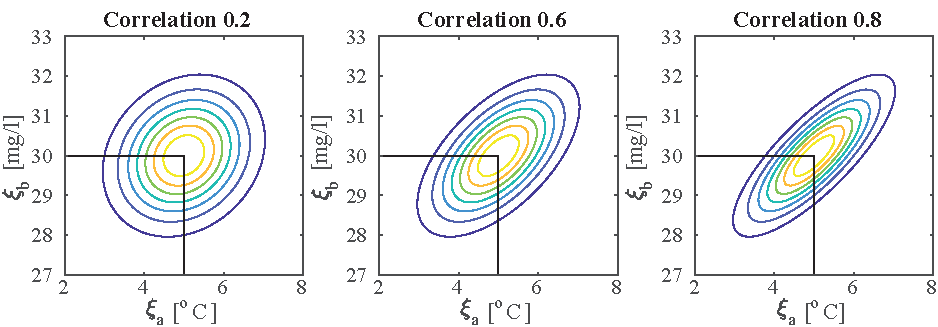
\includegraphics[width=0.99\textwidth]{Figures/illus_bivar.pdf}
  \caption{Density contour plots with different correlations between
    temperature and salinity. The densities have unit variance and the
    thresholds are identical to the mean values $5^o C$ and
    $30 mg/l$. X-axis is temperature and y-axis is salinity.}
\label{illus_bivarDens}
\end{figure}
The displayed densities have unit standard deviations for both
temperature and salinity, but we also study the effect of doubling the
standard deviations.

Table \ref{tab:sim_rhoab} shows the initial EPs and the associated
Bernoulli variance (second row) for the examples indicated in Fig.
\ref{illus_bivarDens}. The EPs increase with the correlation as there
is a strong tendency to have concurrently low temperature and salinity. The Bernoulli variance is similarly large for high
correlations. EPs and Bernoulli variances are the same for standard
deviation $1$ or $2$, which implies that high variability in
temperature and salinity is not captured in the $p(1-p)$ expression.

\begin{table}[!h] \centering \caption{EP and Bernoulli variance for
    different correlations and variances (top rows), and expected
    Bernoulli variances for both temperature and salinity data $\by$ and 
    temperature $y_2$ (bottom rows).}
  \begin{tabular}{c|ccc|ccc}
 &\multicolumn{3}{c}{$\sigma_1=\sigma_2=1$} & \multicolumn{3}{c}{$\sigma_1=\sigma_2=2$} \\
\hline
Correlation $\gamma$ & 0.2 & 0.6 & 0.8 & 0.2 & 0.6 & 0.8 \\
\hline
$p$ & 0.28 & 0.35 & 0.40 & 0.28 & 0.35 & 0.40 \\ 
$p(1-p)$ & 0.20 & 0.23 & 0.24 & 0.20 & 0.23 & 0.24 \\ 
EIBV, Temp and Salinity data & 0.092 & 0.089 & 0.085 & 0.052 & 0.051 & 0.049 \\ 
EIBV, Temperature data only & 0.151 & 0.138 & 0.123 & 0.137 & 0.114 & 0.093 \\ 
\hline
\end{tabular}
\label{tab:sim_rhoab}
\end{table}

Table \ref{tab:sim_rhoab} (bottom two rows) shows results of expected
Bernoulli variance calculations. This is presented for a design
gathering both data types, and for a design with temperature
measurements alone. When both data are gathered, the measurement model is
$(Y_{d,1},Y_{d,2})^t=(Z_1,Z_2)^t+\bepsilon$, with $\bepsilon \sim N(0,0.5^2I_2)$, while $Y_d=Z_1+\epsilon$, $\epsilon \sim N(0,0.5^2)$ when only temperature is measured.
For this illustration, Table \ref{tab:sim_rhoab} shows that the
expected Bernoulli variance gets lower with larger standard deviations
$\sigma_1$ and $\sigma_2$ (right columns). The reduction of Bernoulli
variance is largest for the cases with high correlation
$\gamma$. Albeit smaller, there is also uncertainty reduction when
only temperature is measured (bottom row), especially when temperature
and salinity are highly correlated. When correlation is low
($\gamma=0.2$), there is little information about salinity in the
temperature data, and therefore less uncertainty reduction. In an
application with fresh cold water from a river source, the temperature
and salinity variables will not only be interdependent, but will also
likely show dependence in the spatial dimension. This in turn will
impact the design criteria when we evaluate the information measure by
integrating over several locations (Section \ref{sec:simulations}).

%\subsection{Expected classification criteria}

%{\bf{I have not done anything here - skip this, I think}}.

%Rather than minimizing expected variance one can aim at minimizing the classification probability of the excursion set: 
%$\min [p,(1-p) ]$, see e.g. \cite{lilleborge2016information}. 

%Again, since the conditional mean is a linear in the data, we only have to look at the %relevant linear combination via $\bm_{\xi}=E(\bxi)$.
%See also \cite{bhattacharjya2013value}.

%\begin{equation}
%E(\min \{ p,(1-p)\})=\int \min P(\xi_1 \leq t, \xi_2 \leq s),[1-P(\xi_1 \leq t, \xi_2 \leq s)] p(E(\bxi)=) dE(\bxi)=,
%\end{equation}
%for the complementary probabilities, this is again evaluated by the corner regions for the block, and $\Phi_4()$ evaluations are required.

%In the end, this result is integrated over the spatial domain $x \in X$.

\section{Sequential designs and heuristic path planning}\label{sec:heuristics}

An important concept underlying this work is the potential of robotic
sampling to adapt survey plans based on data and statistical methods
in accordance with the sense-plan-act control loop
(Fig. \ref{fig:envir1}). We now present a few adaptive strategies for
robotic sampling that build on the notion of EIBV.

\subsection{Optimal Sequential Design}
\label{Optdes}

Our adaptive AUV survey is split into many stages. The selection on
where to sample is constrained by a triangular waypoint graph and
defined by its nearest grid nodes.

Let $d^{j,s}$ denote design number $j$ at stage $s$ of a sequential
survey. For the AUV sampling situation, the choice of design entails a commitment to one of many possible navigation directions on the waypoint graph. Once the choice has been made, the AUV steers in the chosen direction and this entails sampling locations $\bu_{d^{j,s}}$ and data $\by_{d^{j,s}}$ is gathered.  We let
$\mathcal{Y}^{s-1} =\{(d^{*,1}, \by_{d^{*,1}}),\ldots, (d^{*,s-1},
\by_{d^{*,s-1}}) \}$ denote the set of all data gathered until stage
$s-1$ according to selected design $d^{*,1},\ldots,d^{*,s-1}$.  

The design and data define
the conditional GP with mean
$E(\gp[\x]|\mathcal{Y}^{s-1})$ and (cross) covariance matrix
$\mbox{Var}(\gp[\x]|\mathcal{Y}^{s-1})$. These are efficiently updated in a sequential manner keeping track of the mean and covariance kernel of the GP over the stages. As extensions of Eq. \eqref{eq:cokrig} and \eqref{eq:krig:cov}, we have
\begin{eqnarray}\label{eq:krigSUR}
\mu^{s}(\x) &=&\mu^{s-1}(\x)+\lambda^{[s,s]}(\x,\bu_{d^{j,s}})^T (\by_{d^{j,s}}-G_{d^{j,s}} \mu(\x)), \nonumber \\
k^{s}(\x,\x') &=& k^{s-1}(\x,\x')-\lambda^{[s,s]}(\x,\bu_{d^{j,s}})^T K_{Y_{d^{j,s}}} \lambda^{[s,s]}(\x',\bu_{d^{j,s}}),
\end{eqnarray}
where $\lambda^{[s,s]}(\x,\bu_{d^{j,s}})=K^{-1}_{Y_{d^{j,s}}} G_{d^{j,s}} k(\bu_{d^{j,s}},\x)$ and the data covariance is $K^{-1}_{Y_{d^{j,s}}}=G_{d^{j,s}} K^s(\bu_{d^{j,s}},\bu_{d^{j,s}})G^T_{d^{j,s}}+R_{d^{j,s}}$, with measurement model as in Eq. \eqref{eq:meas}.

At stage $s$, the robot must then choose design $d^{j,s}$ where measurements $\by_{d^{j,s}}$ should
be gathered. For the triangularized waypoint
graph all six possible
directions must be evaluated to minimize the expected uncertainty of random sets, and in particular the EIBV for our 
application. We hence focus on choosing designs for data modeled by
Eq. \eqref{eq:meas}, to conduct efficient sequential uncertainty
reduction according to the EIBV criterion. Compared with the
static design $d$ in Eq. \eqref{eq:eibv}, the optimal sequential
design not only considers the best current design grid point, but also
how the data gathered at this node could inform future sampling at
successive stages.

%The optimal path
%selection situation is depicted in Fig. %\ref{fig:PathSelOpt},
%\begin{figure}[b!]
%\centering
%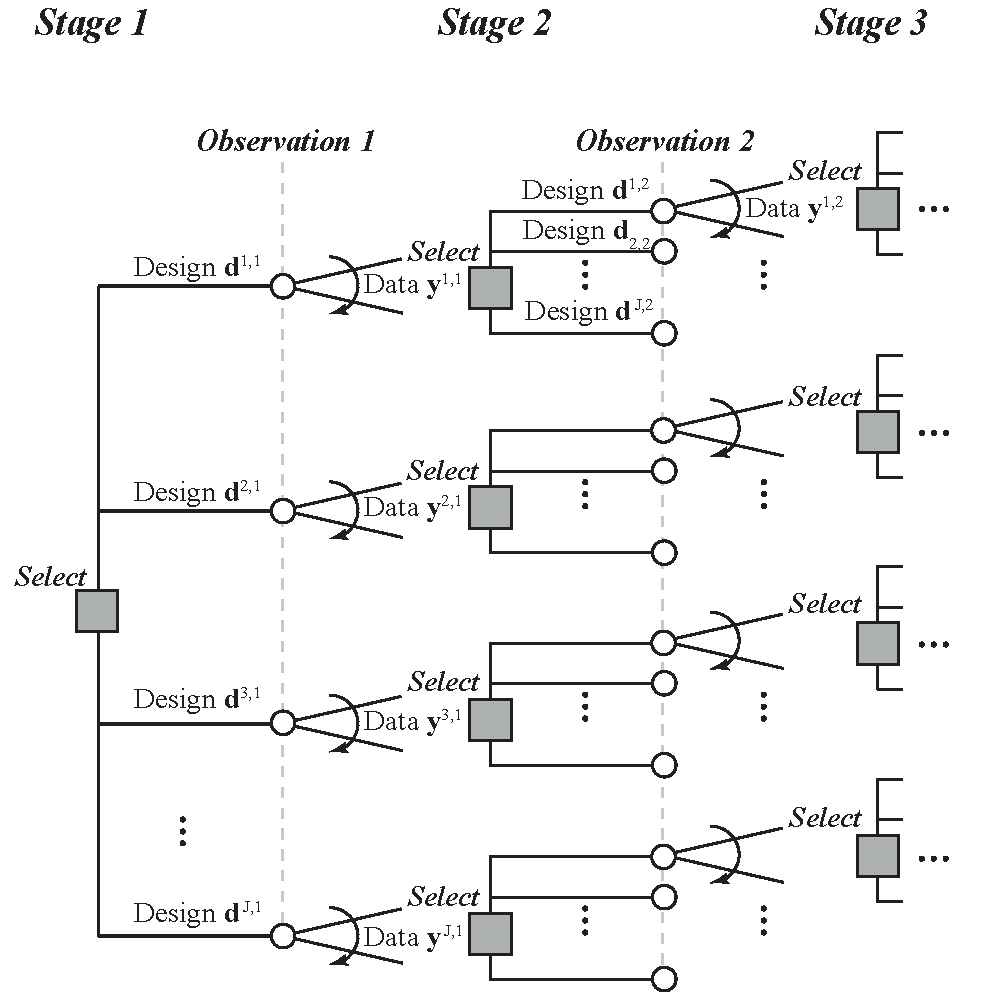
\includegraphics[width=0.85\textwidth]{Figures/sequent_select.pdf}
%\caption{Optimal sequential path selection.}\label{fig:PathSelOpt}
%\end{figure}
%where design choices are indicated by squares while %data realizations are indicated by circles. 
%terms this optimal design is defined as
%\begin{equation}\label{opt_crit}
%    \bd^* = \mbox{argmin}_{d^{j,1}} \left\{ \int_{\by^{j,1}} \mbox{argmin}_{d^{j,2}} \left\{ \int_{\by^{j,2}} \ldots \pi(\by^{j,2}|\by^{j,1}) d\by^{j,2} \right\} \pi(\by^{j,1}) d \by^{j,1} \right\},
%\end{equation}
%where $\ldots$ represents the expected variance reduction in the ES under the continued optimal design, which will depend on the data at earlier stages. 
The mathematical expression for the optimal design involves a series
of intermixed maximizations over designs and integrals over data. In
practice, the optimal solution is intractable because of the enormous
growth over stages (see e.g. \cite{sucar2015probabilistic} and
\cite{powell2016perspectives}).  Instead, we outline heuristic
strategies.


%The derived closed-form solutions for the EIBV are still important building blocks when constructing the sampling designs, as they will be used to score the different adaptive designs. % Efficient
% calculation is important for using adaptive survey designs with
% robotic platforms.
 
\subsection{A Naive Sampling Strategy}
\label{naive}

The simplest heuristic for adaptive sampling is to choose the next
sampling location based on current probabilities. One reduces the
largest levels of uncertainty by selecting the design $j$ with
$P(Z(\x_j) \in T)$ closest to $0.5$.  With temperature and salinity
variables, this {\it{naive}} strategy selects the stage $s$ sampling
design according to:
\begin{eqnarray}\label{critNaive}
    d^{*,s} &=& \mbox{argmin}_{j} |P(Z_1(\x_j) \leq t_1, Z_2(\x_j) \leq t_2 | \mathcal{Y}^{s-1})-0.5|, \nonumber
\end{eqnarray}
where $j$ is indexing all neighboring locations on the waypoint graph.

This strategy does not account for the uncertainty in the GP
variables, but is instead applicable only if one design (node) has EPs
closer to $0.5$ (see Table \ref{tab:sim_rhoab}, row
two). Additionally, this strategy does not account for spatial
correlation. This strategy lacks memory of where it has been and where
the uncertainty has been reduced, and therefore susceptible to local
minima.

\subsection{Myopic Path Planning}
\label{sec:myopic}

The myopic (greedy) strategy which we present here is optimal if we
imagine taking only one more stage of measurements. This selection
strategy is based on expected uncertainty reduction, but it is a
heuristic because there is no anticipation of what the subsequent
designs might offer beyond the first stage.

Based on the currently available data $\mathcal{Y}^{s-1}$, we fit an
updated GP model. Focusing on the EIBV criterion, at the next stage
$s$, the selected design is:
\begin{eqnarray}\label{critSEQ}
    d^{*,s} &=& \mbox{argmin}_{j} \left\{ \int_{\mathcal{M}} E_{\by_{d^{j,s}}|\mathcal{Y}^{s-1}} \left( p(\x;\mathcal{Y}^{j,s})\left( 1-p(\x;\mathcal{Y}^{j,s})\right) \right) d\mes(u), \right\} \\
    p(\x;\mathcal{Y}^{j,s}) &=& P(Z_u \in T |\by_{d^{j,s}},\mathcal{Y}^{s-1}). \nonumber
\end{eqnarray}

Note that this strategy gives a sequential conditional version of
expression (\ref{eq:eibv}). Now $\mathcal{Y}^{s-1}$ is available, and
the expectation is conditional to this data. A similar closed-form
calculation for EIBV is hence applicable in Eq.  \eqref{critSEQ} using the updated
GP model from stage $s-1$ as defined via Eq. \eqref{eq:krigSUR} in the results from Proposition \ref{propo2}. Once the data are collected for the best design $d^{*s}$ at stage $s$, the GP model is updated again. The mean and covariance are used to compute the next design at stage $s+1$, and so on.

Even though this myopic strategy is non-anticipative, it still gives a
reasonable approach for creating designs in many
applications. Moreover, it is easily implemented, in our case, onboard
an AUV, using an efficient data update of the GP model and the
calculation of the closed-form EIBV expressions for each subsequent
trajectory.


\subsection{Look-ahead Trajectory Planning}
\label{sec:LA}

We now extend the myopic strategy to a look-ahead strategy. We consider two stages of
measurements, and the strategy is then optimal in the sense that it accounts consistently for the expectations and minimizations in these two stages, but still without including any planning beyond those two steps. In addition to the
next stage of measurements $\by^{j,s}$, this look-ahead strategy anticipates the subsequent design indexed $j_2$ with data
$\by^{j_2,s+1}$ when choosing the current design $d^{j,s}$. The
selected design is:
\begin{eqnarray}\label{critLA}
    d^{*,s} &=& \mbox{argmin}_{j} \left\{ E_{\by_{d^{j,s}}|\mathcal{Y}^{s-1}} \left( \mbox{argmin}_{j_2}  V_{j_2} \right) \right\}, \\
V_{j_2} & = & \int_{\mathcal{M}} E_{\by_{d^{j_2,s+1}}|\mathcal{Y}^{j,s}} \left( p(\x;\mathcal{Y}^{j,s+1}) ( 1-p(\x;\mathcal{Y}^{j,s+1}) ) \right) d\mes(u), \nonumber \\
    p(\x;\mathcal{Y}^{j,s+1}) &=& P(Z(\x) \in T |\by_{d^{j_2,s+1}},\mathcal{Y}^{j,s}). \nonumber
\end{eqnarray}
Here, $\mathcal{Y}^{j,s}=\{\by_{d^{j,s}},\mathcal{Y}^{s-1}\}$ and
$\mathcal{Y}^{j,s+1}=\{\by_{d^{j_2,s+1}},\mathcal{Y}^{j,s}\}$
represent the sets of data variables, and the expectations are
calculated with respect to the conditional densities given data at
that stage.  We solve the first expectation by Monte
Carlo sampling of data $\by_{d^{j,s}}$ from its conditional
distribution. For each of these data samples, the second expectation
is solved using the closed-form expressions for EIBV using the results from Proposition \ref{propo2}, now with conditioning to the first stage data already going into the mean and covariances in Eq. \eqref{eq:krigSUR}. 

Even though the strategy looks at two sampling stages, it is only used to find
the current best design. When data are collected at stage $s$, the GP model is
updated as in Eq. \eqref{eq:krigSUR}, and the mean and (cross) covariance are
used to compute the next design for stage $s+1$, now anticipating what
stage $s+1$ and $s+2$ could offer, and so on.
This look-ahead approach is much more computationally demanding than
the myopic strategy, so for practical implementation onboard the AUV this is reaching the limits allowed for calculation. We conduct some pruning of the least valuable design paths in the evaluation of Eq. \eqref{critLA}, to get a satisfactory computation time below one minute per waypoint. This means that we use the myopic
strategy to rank the three best designs following the first stage alone, and
for each of these preferred designs, we undertake the look-ahead calculations.

\section{Simulation study}
\label{sec:simulations}

We now study the properties of the different static and sequential
survey designs in a realistic case that emulates the spatial
properties of a river plume interacting with coastal water.

\subsection{Modeling}

A GP model is used to represent the bivariate random fields of
temperature and salinity. At location $\x \in \mathcal{M}$, the
bivariate distribution is:
\begin{equation}\label{gp_bar}
\begin{bmatrix}Z_1(\x) \\
Z_2(\x) \end{bmatrix}
\sim N \left( 
\begin{bmatrix} \mu_{1}(\x)\\
\mu_{2}(\x)
\end{bmatrix},\begin{bmatrix}
\sigma_{1}^2 & \sigma_{1} \sigma_2 \gamma \\
\sigma_{1} \sigma_2 \gamma  & \sigma_{2}^2 
\end{bmatrix}
\right).
\end{equation}
We specify the mean by $\mu_{1}(\x)=5.8 + 0.065 u_{\mbox{West}}$ and
$\mu_{2}(\x)=29 + 0.1 u_{\mbox{West}}$, which means that the expected
levels of both temperature and salinity increase linearly in the
western direction.  This situation mimics that of a river mouth
opening from the south, with the water masses pulled to the east by
the Coriolis force \kc{This seems overly specific to the Nidelva use
  case. Can it be generalized, after all that is the overall intent of
  this manuscript?}.  The variances are set to $\sigma_1=0.25$ and
$\sigma_2=0.6$, while the correlation is $0.6$.  The spatial
correlation is of separable Matern type (see e.g. \cite{Cressie:11})
so that
\begin{equation}\label{v}
\small
\mbox{Corr} 
\left(
\begin{bmatrix}
    Z_1(\x) \\
    Z_2(\x) 
    \end{bmatrix},
    \begin{bmatrix}
    Z_1(\x') \\
    Z_2(\x') 
    \end{bmatrix}
    \right)
    = \begin{bmatrix}
1 & 0.6  \\
0.6  & 1
\end{bmatrix}(1+\phi h)\exp (-\phi h),
\end{equation}
where $h=\sqrt{||\x-\x'||^2}$ and $\phi=0.3$ indicates an effective
correlation range of about $1200$ m.

In the accompanying Python code, these modeling assumptions can be
generalized to anisotropic covariance and changing variance levels
across the spatial domain. One can hence, easily run the code to see
if different models result in other sampling designs. Anisotropy and
non-stationary variance are both relevant for the setting with river
plumes, but in practice this requires more parameters to be
specified. With extensive data and prior knowledge, one could also
possibly fit and estimate parameters of more complex multivariate
spatial covariance functions
\citep{gneiting2010matern,genton2015cross}, but that is outside the
scope of the current paper.

We discretize the spatial domain $\mathcal{M}$ to a set of $n$ grid
locations $\mathcal{M}_g = \{\x_i, i=1,\ldots,n \}$, \kc{is the index
  correct? TeX shows it as u or g for $\mathcal{M}$} where each cell
has area $\Delta$; the same grid is used for the waypoint graph for
possible design locations. The EIBV is approximated by sums over all
grid cells.

One realization of the random fields representing salinity and
temperature is shown in Fig. \ref{fig:true_temp} and
\ref{fig:true_sal}. The true ES is a realization from this model as
shown in Fig. \ref{fig:ESet}.

\begin{figure}[!h]
  \centering
  \subfigure[Simulated temperature.]{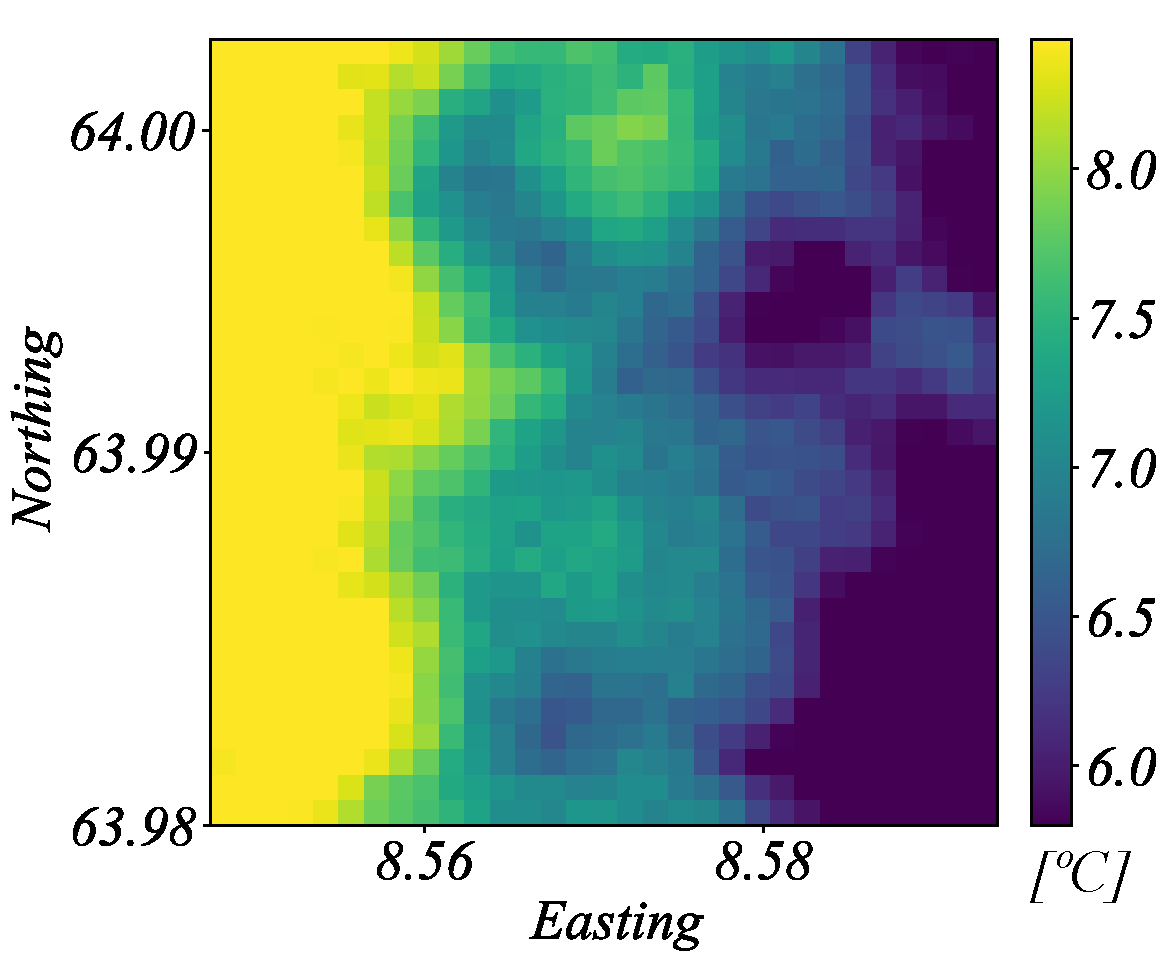
\includegraphics[height = 0.40\textwidth]{Figures/sim/true_temp.pdf}\label{fig:true_temp}}
  \hfill
  \subfigure[Simulated salinity.]{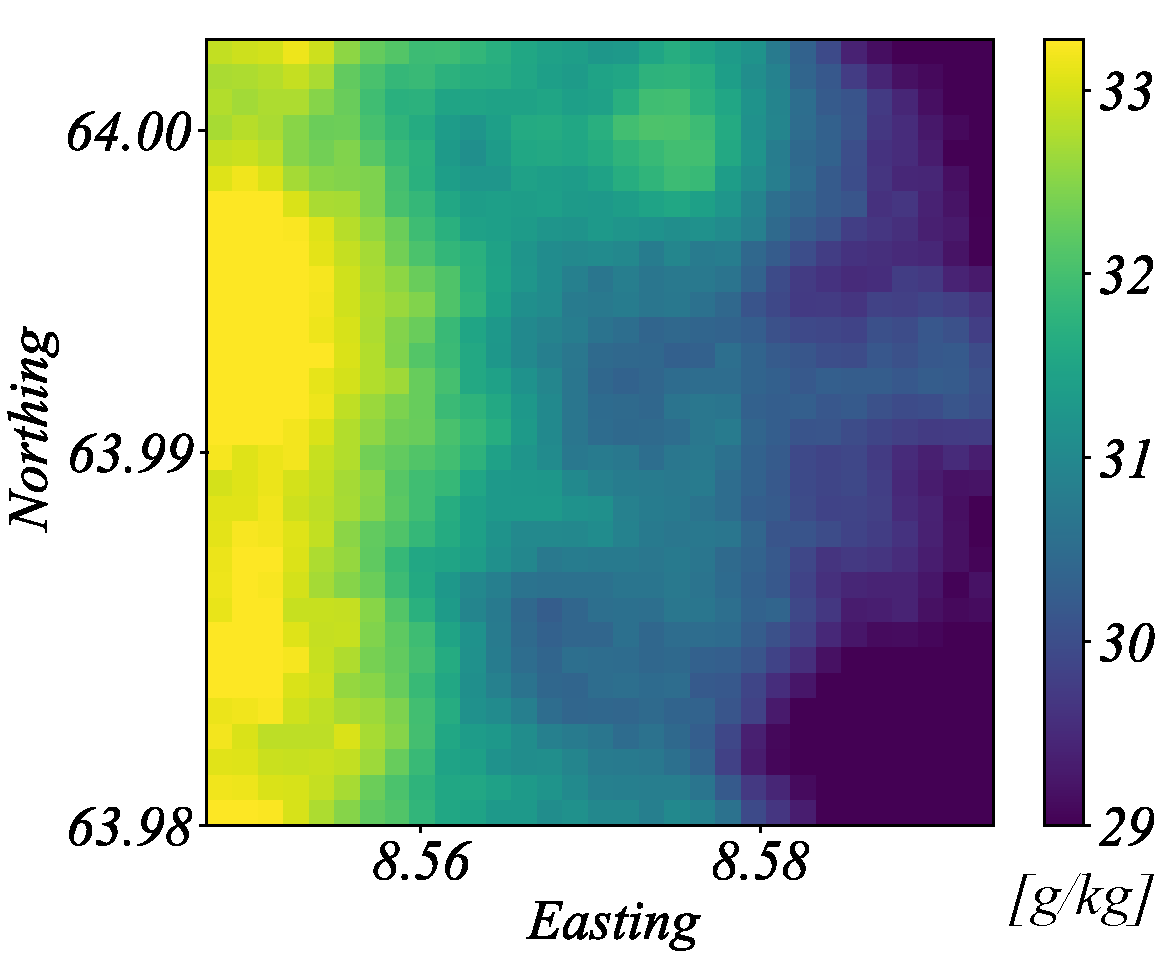
\includegraphics[height = 0.40\textwidth]{Figures/sim/true_sal.pdf}\label{fig:true_sal}}
  \hfill
  \subfigure[Excursion set given the realization of temperature and salinity.]{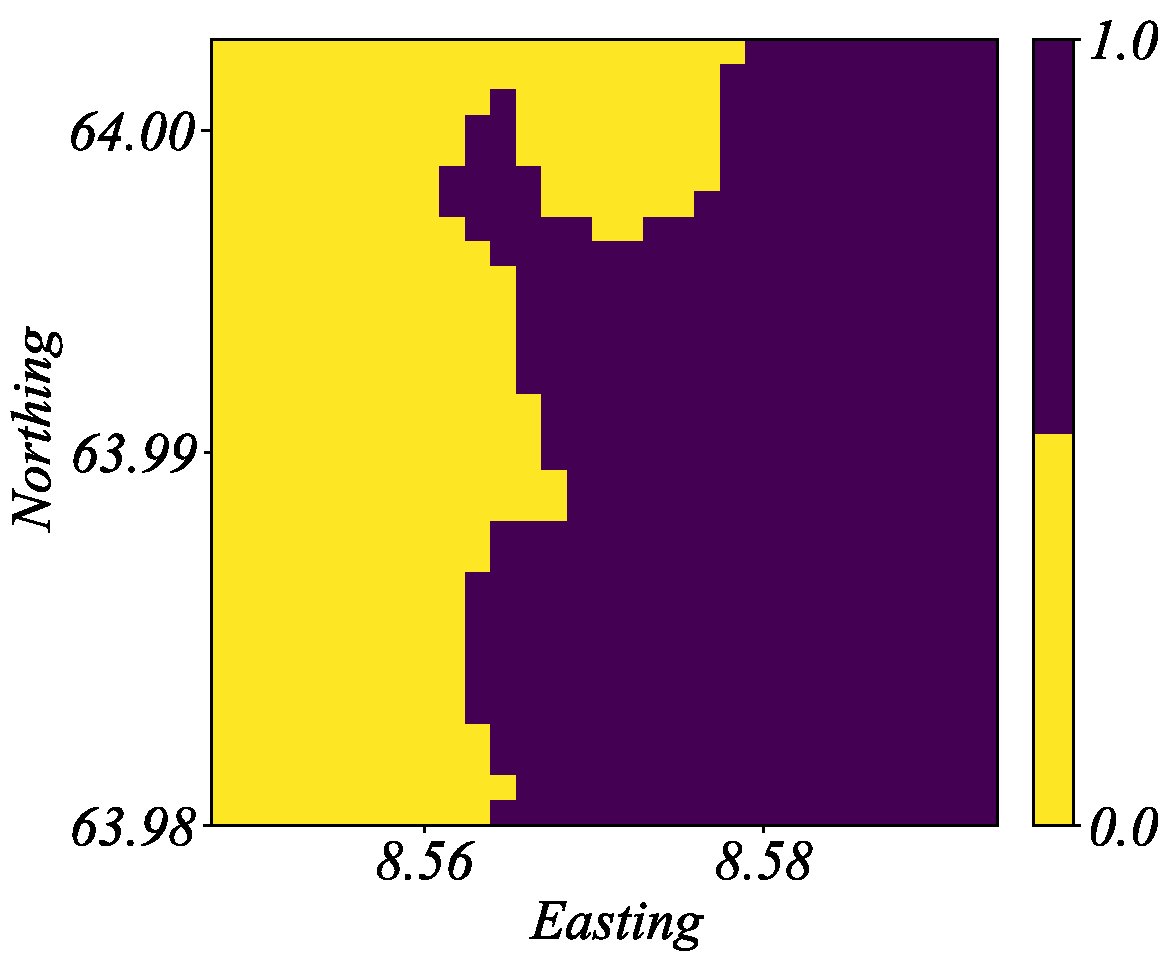
\includegraphics[height = 0.40\textwidth]{Figures/sim/es_ts_true.pdf}\label{fig:ESet}}
  \hfill
  \subfigure[Excursion probabilities given collected data using the
  `static\_north" strategy.]{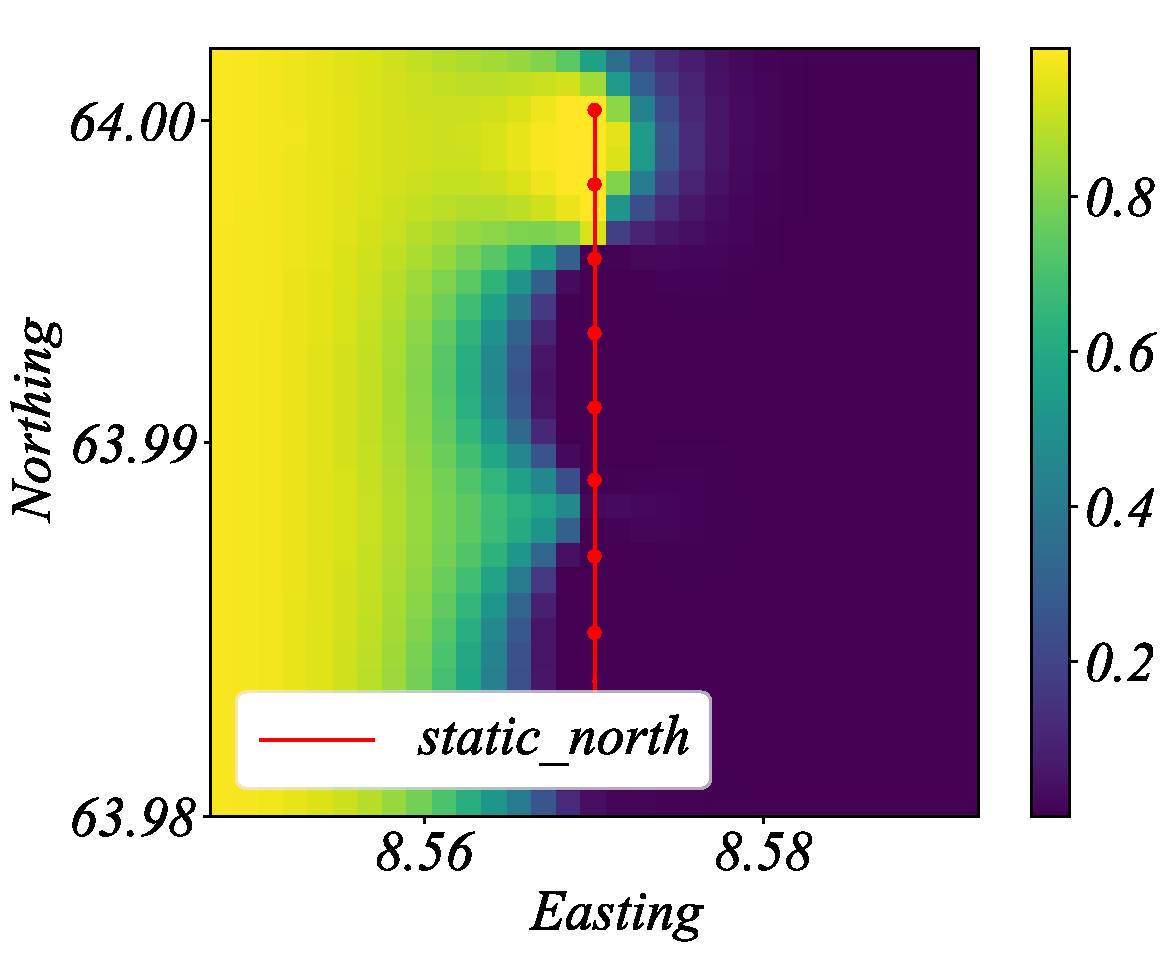
\includegraphics[height = 0.40\textwidth]{Figures/sim/es_ts_posterior.pdf}\label{fig:Eprob}}
  \caption{\ref{fig:true_temp} and \ref{fig:true_sal} show a
    realization of the simulated temperature and salinity fields. The
    associated ES is in \ref{fig:ESet}, while \ref{fig:Eprob} shows
    the estimated EPs after performing data collection along the
    static N-S survey line.}
\label{fig:realisations}
\end{figure}

\subsection{Static and Sequential Sampling Designs}
\label{sec:sampling_designs}

%Three different designs are considered as indicated in Figure \ref{fig:stat_design}. 
%\begin{figure}[h!]
%\centering
%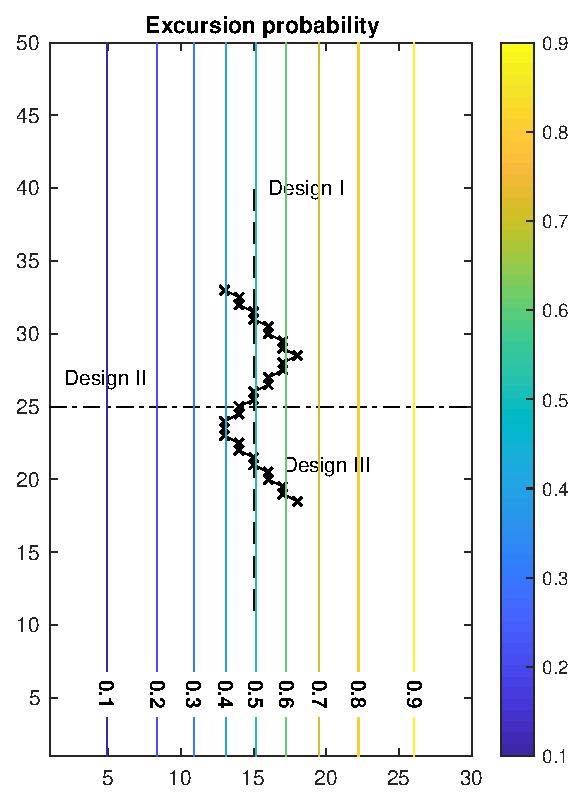
\includegraphics[width=0.65\textwidth]{Figures/Des3.eps}
%\caption{Three different static survey designs plotted on the initial EP.}\label{fig:stat_design}
%\end{figure}
%In this display the designs are plotted along with the prior probability contours of the ES for the reference parameter inputs. 

We compare three different static designs denoted
\textit{static\_north}, \textit{static\_east}, and
\textit{static\_zigzag} with the three described sequential approaches
\textit{naive}, \textit{myopic}, and \textit{look-ahead}. The static
sampling paths are pre-determined and cannot be altered and represent
the pre-planned strategies used in most current AUV operational survey
designs.

For a fixed survey length, a closed-form expression for the EIBV is
available as in Eq. \eqref{eq:eibv}. However, for the sequential
approaches this is not the case. For comparison the properties are
therefore evaluated using Monte Carlo sampling over several replicates
of realizations from the model while conducting simulated sequential
surveys for each one. Fig. \ref{fig:Eprob} shows the conditional EP,
given data gathered along the north-south survey lines in these
displays. In the Monte Carlo replicates, such results are repeatedly
computed to approximate the EIBV. We also compare predictive
performance measured by root mean square error (RMSE) for temperature
and salinity estimates as well as also the variance reduction in these
two variables. It is important to note that the objective function
used by the agent \kc{First of 'agent'. Define it or change it
  to 'robot'? Note further uses below.} is focused on reducing the
EIBV, but we nevertheless expect that we will achieve good predictive
performance for criteria such as RMSE as well. Another non-statistical
criteria that is important for practical purposes is the computational
time needed for the strategy, as this will impact the performance for
an embedded system.

%\begin{figure}[h!]
%\centering
%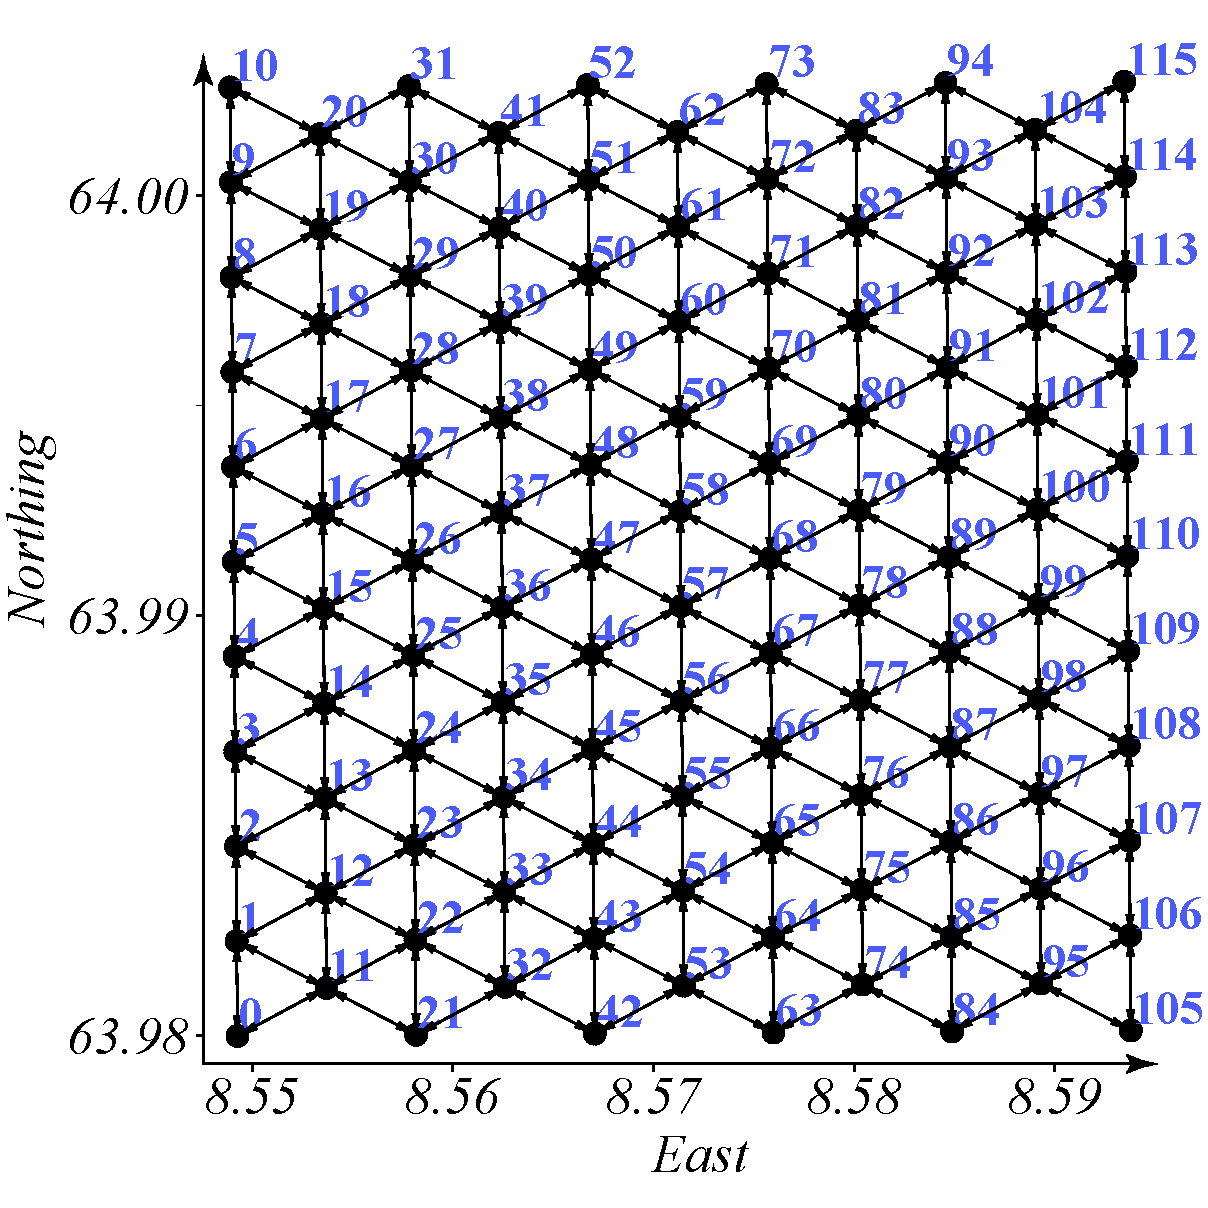
\includegraphics[width=0.50\textwidth]{Figures/sim/wp_graph_paper.pdf}
%\caption{The equilateral waypoint graph used to discretize the
%  trajectory choices over the $31\times31$ grid used to discretize the GP.}
%\label{fig:wp_graph}
%\end{figure}

\begin{figure}[!h] 
\centering 
\subfigure[The waypoint graph.]{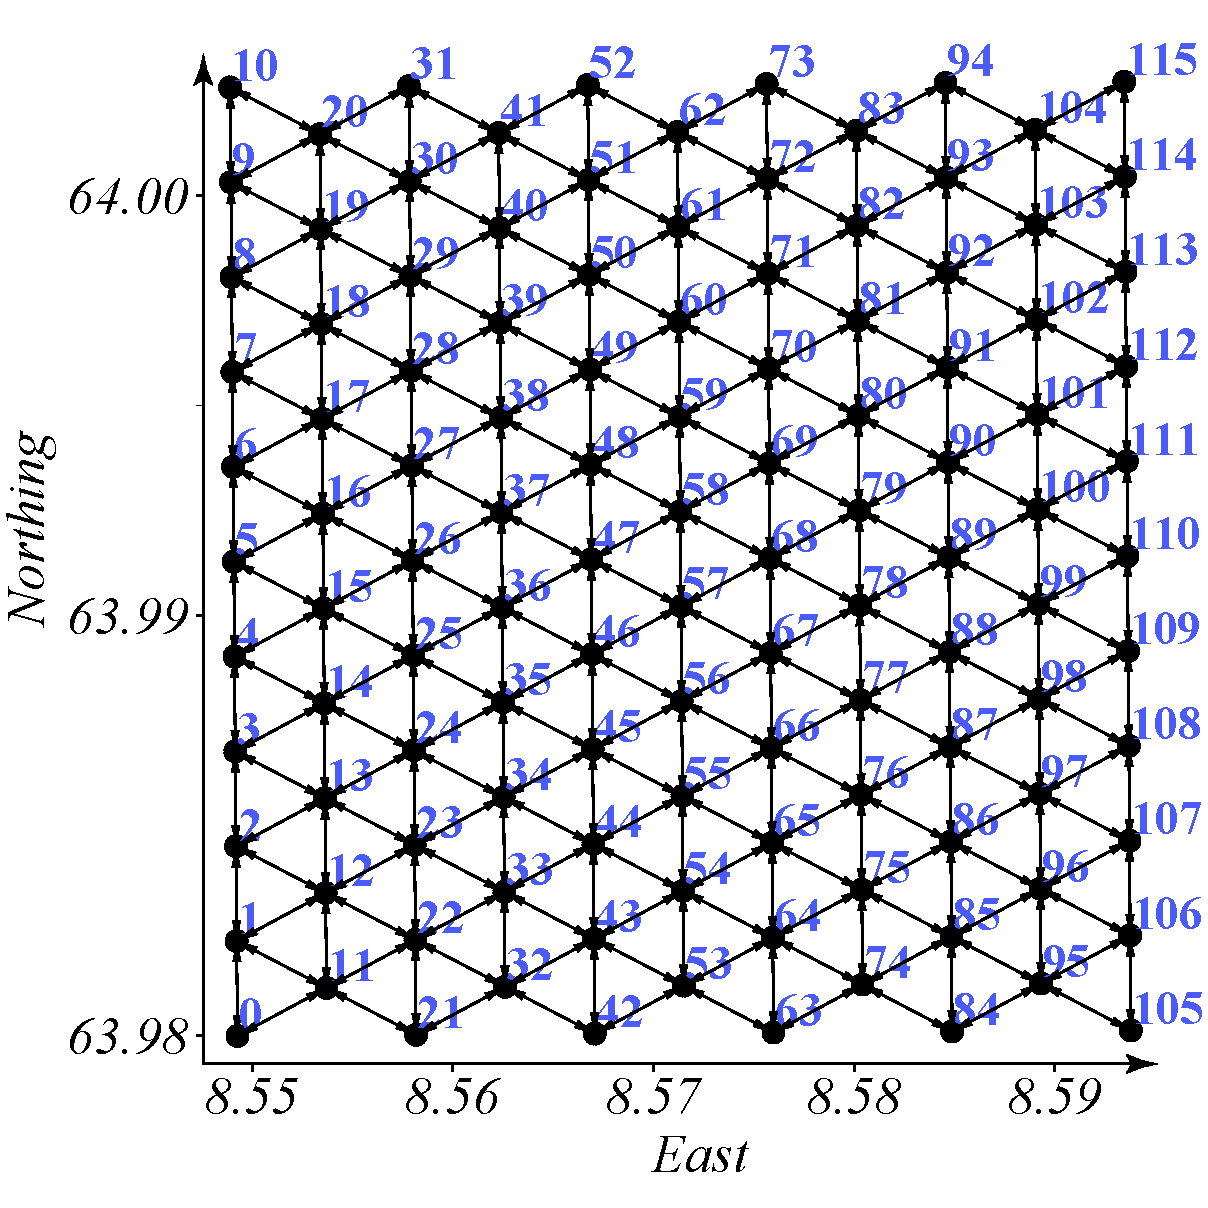
\includegraphics[width =
0.49\textwidth]{Figures/sim/wp_graph_paper.pdf}\label{fig:wp_graph_a}}
\hfill
\subfigure[The waypoint graph in 3D.]{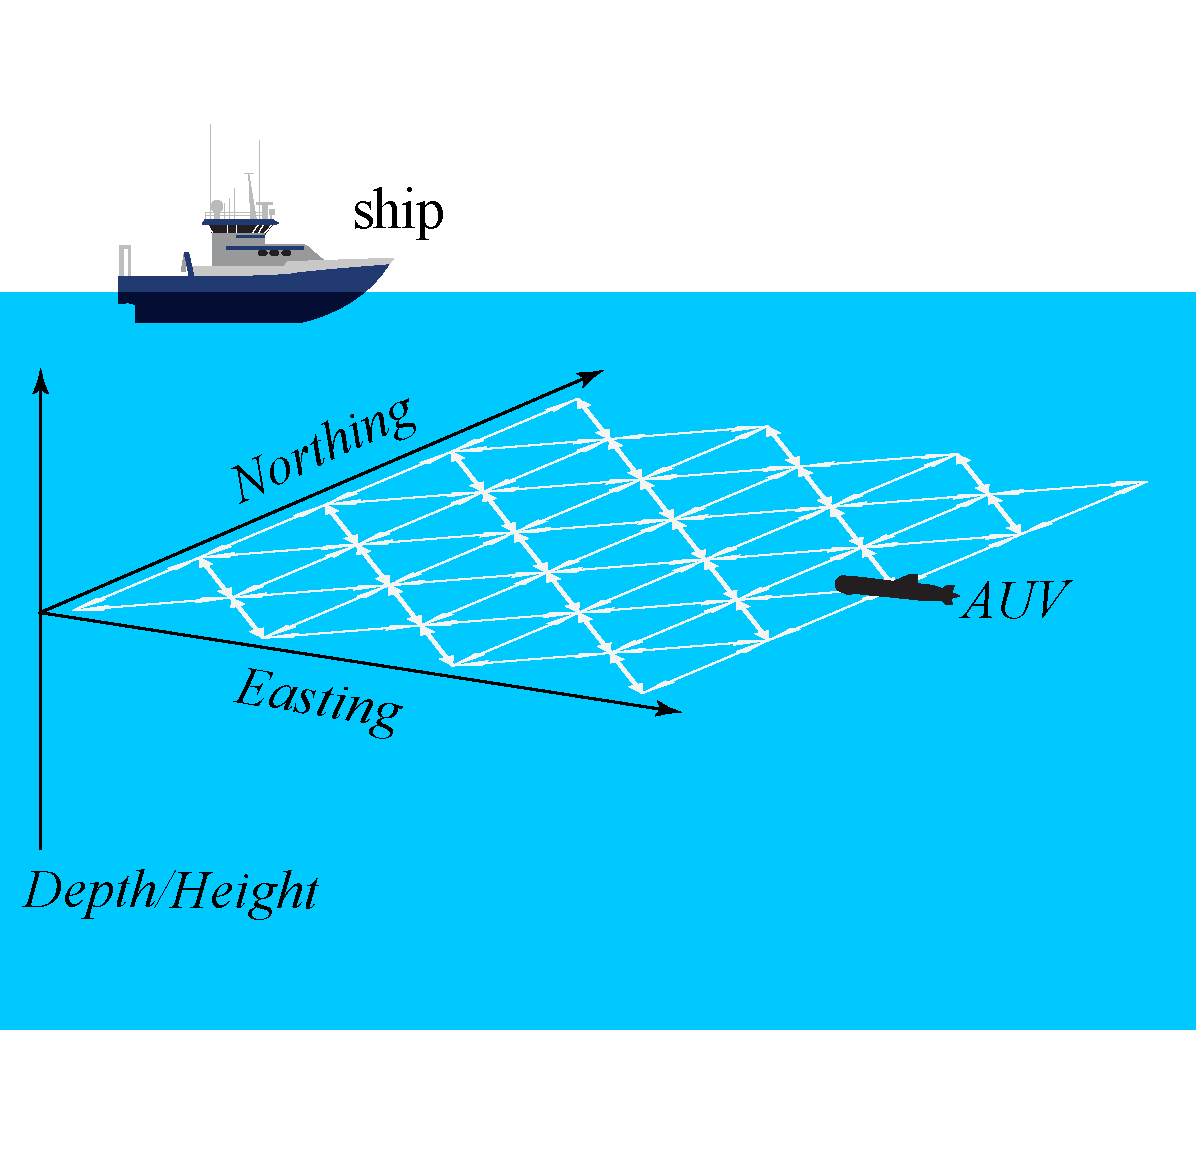
\includegraphics[width =
0.49\textwidth]{Figures/sim/wp_graph_3d.pdf}\label{fig:wp_graph_b}}
\caption{\ref{fig:wp_graph_a} The equilateral waypoint graph used to discretize the
trajectory choices over the $31\times31$ grid used to discretize the GP.
\ref{fig:wp_graph_b} The waypoint grid shown in a 3D environment.}
\label{fig:wp_graph}
\end{figure}

Each strategy is conducted on an equilateral grid as shown in
Fig. \ref{fig:wp_graph}. The sequential sampling agent starts at the
center East-West coordinate at the southern end of the domain (node 53
\kc{Maybe color this node differently and modify the caption?}). The
AUV moves along edges in the waypoint graph while the vehicle makes
measurements. The data is assimilated into the GP model before an
evaluation of the next node to sample is conducted at the end of the
edge.

\subsection{Simulation Results}

A total of 100 replicate simulations were conducted with all
strategies. The results are shown in Fig. \ref{fig:sim_results}, where
the different criteria are plotted as a function of survey
distance. Fig. \ref{fig:avg_ev} shows the resulting drop in IBV for
each of the six strategies. IBV reduction occurs most under the
\textit{myopic} and \textit{look-ahead} strategies, each performing
almost equally; this is expected as the two criteria
(Eq. \eqref{critSEQ} and \eqref{critLA}) are sensitive to differences
in IBV. The \textit{static\_north} design also does well here because
the path is parallel to the boundary between the water masses.

\begin{figure}[h!]
  \centering
  % \subfigure[Excursion set variance $E_{\by}(p[1-p])$.]{\label{fig:avg_ev}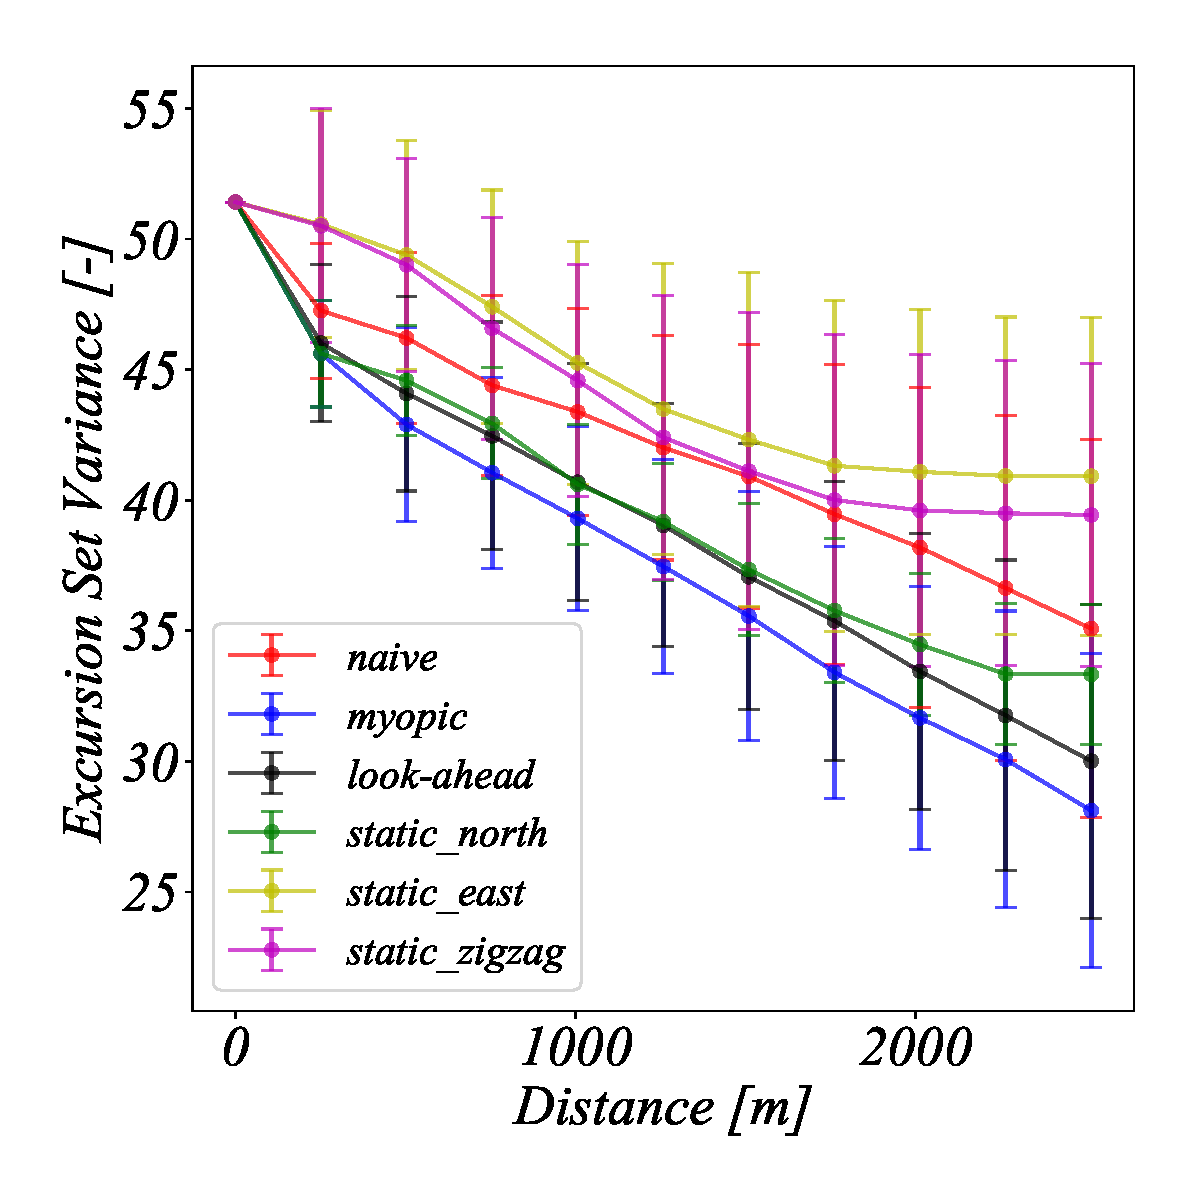
\includegraphics[height=0.49\textwidth]{Figures/sim/avg_EV.pdf}}
  \subfigure[IBV.]{\label{fig:avg_ev}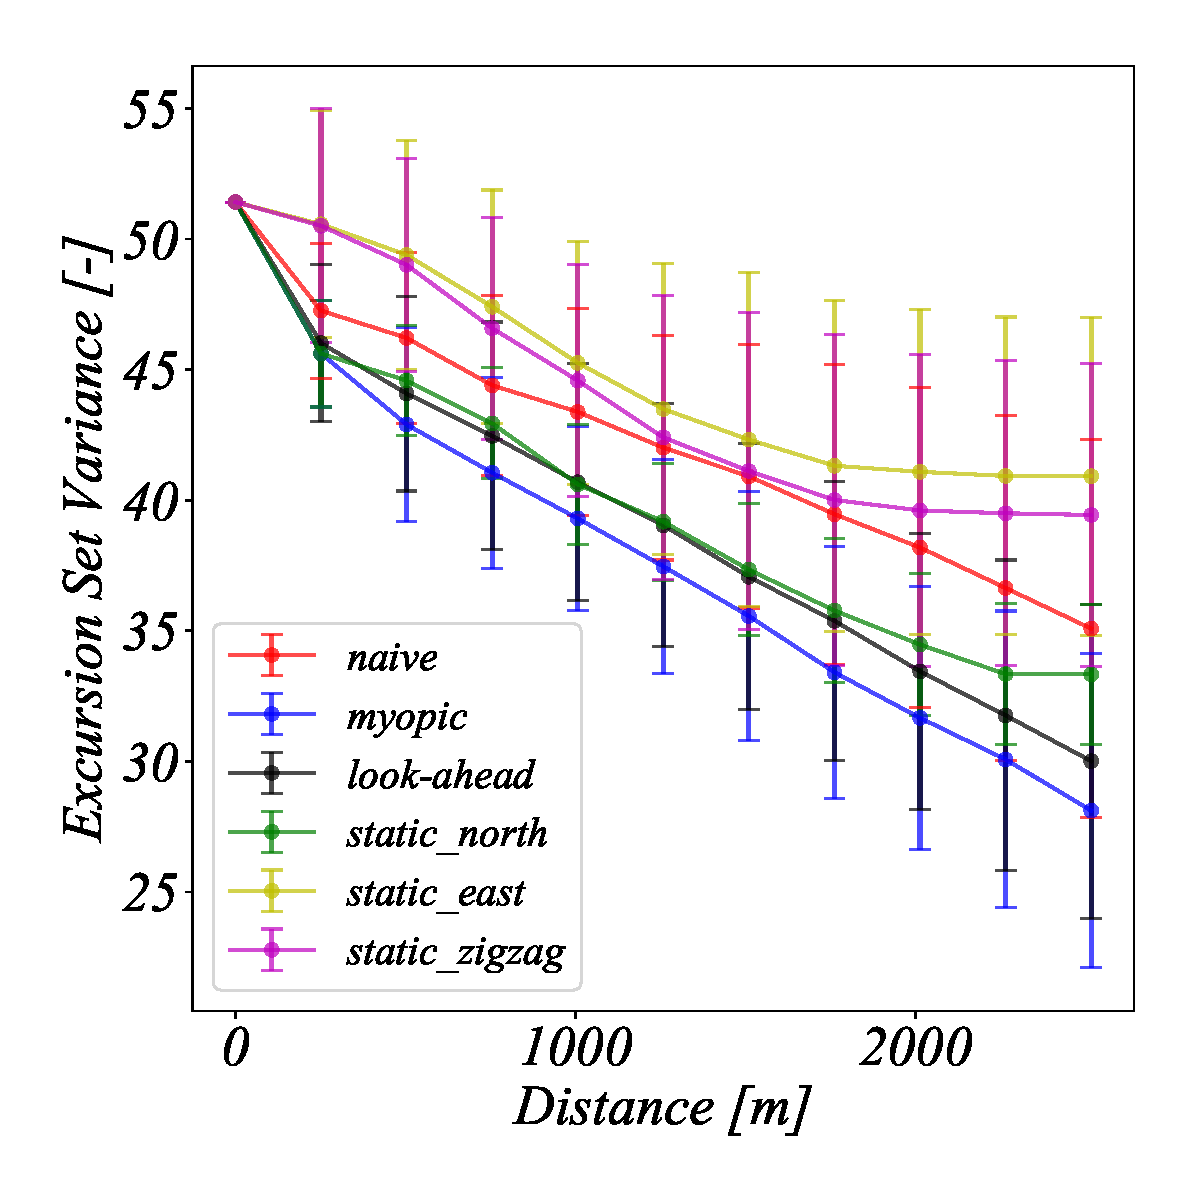
\includegraphics[height=0.49\textwidth]{Figures/sim/avg_EV.pdf}}
  \hfill
  \subfigure[RMSE between estimated field and truth.]{\label{fig:avg_rmse}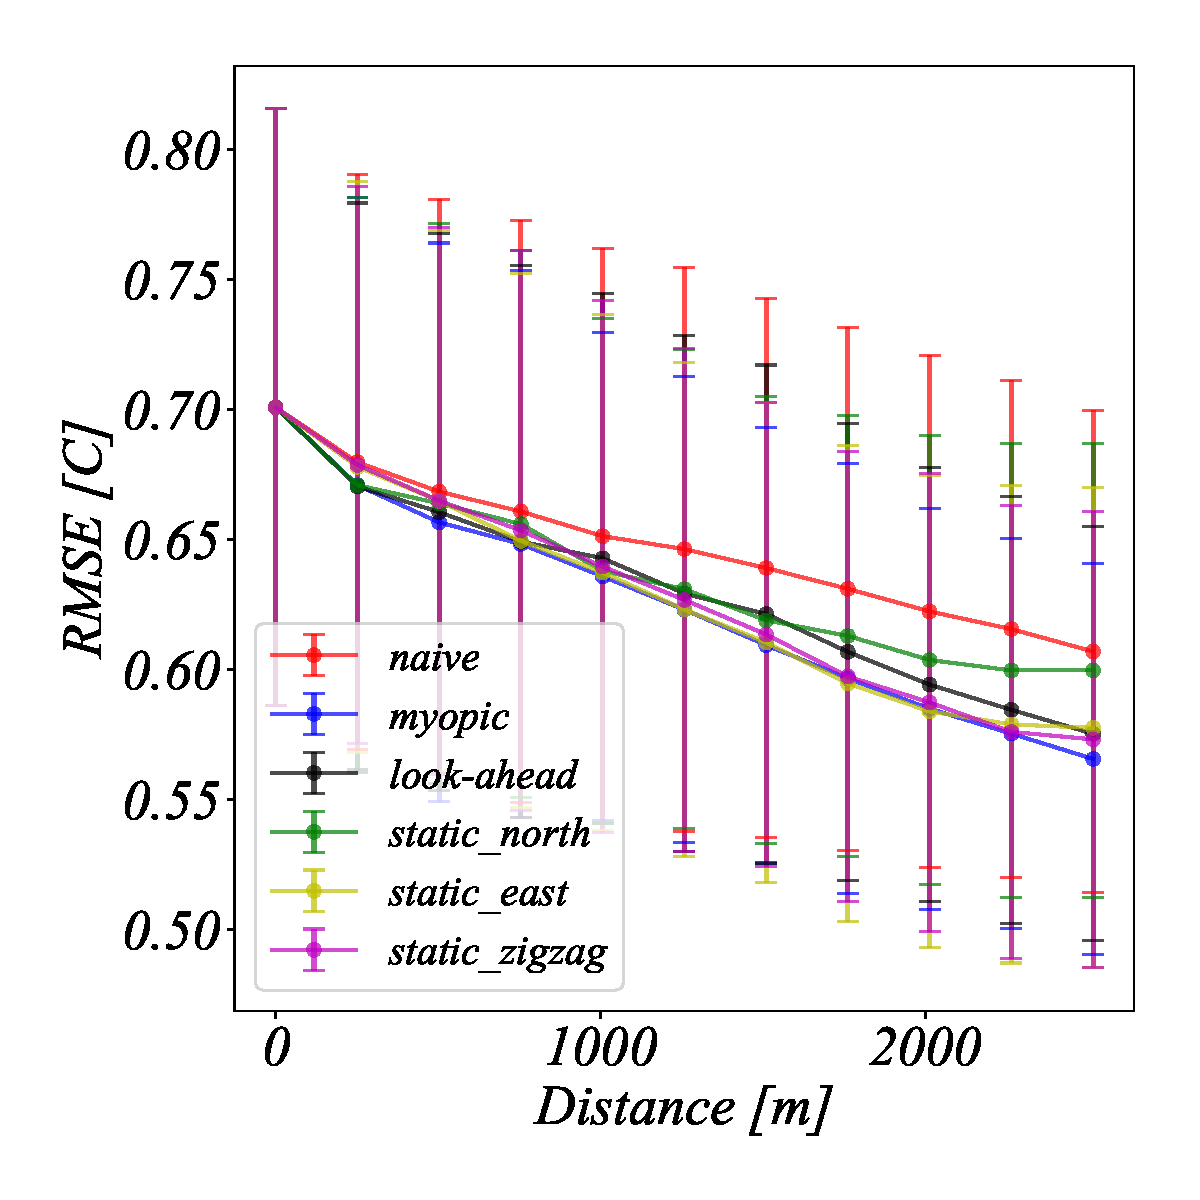
\includegraphics[height=0.49\textwidth]{Figures/sim/avg_RMSE.pdf}}
  \hfill 
  \subfigure[Explained variance $\bR^{2}$.]{\label{fig:avg_r2}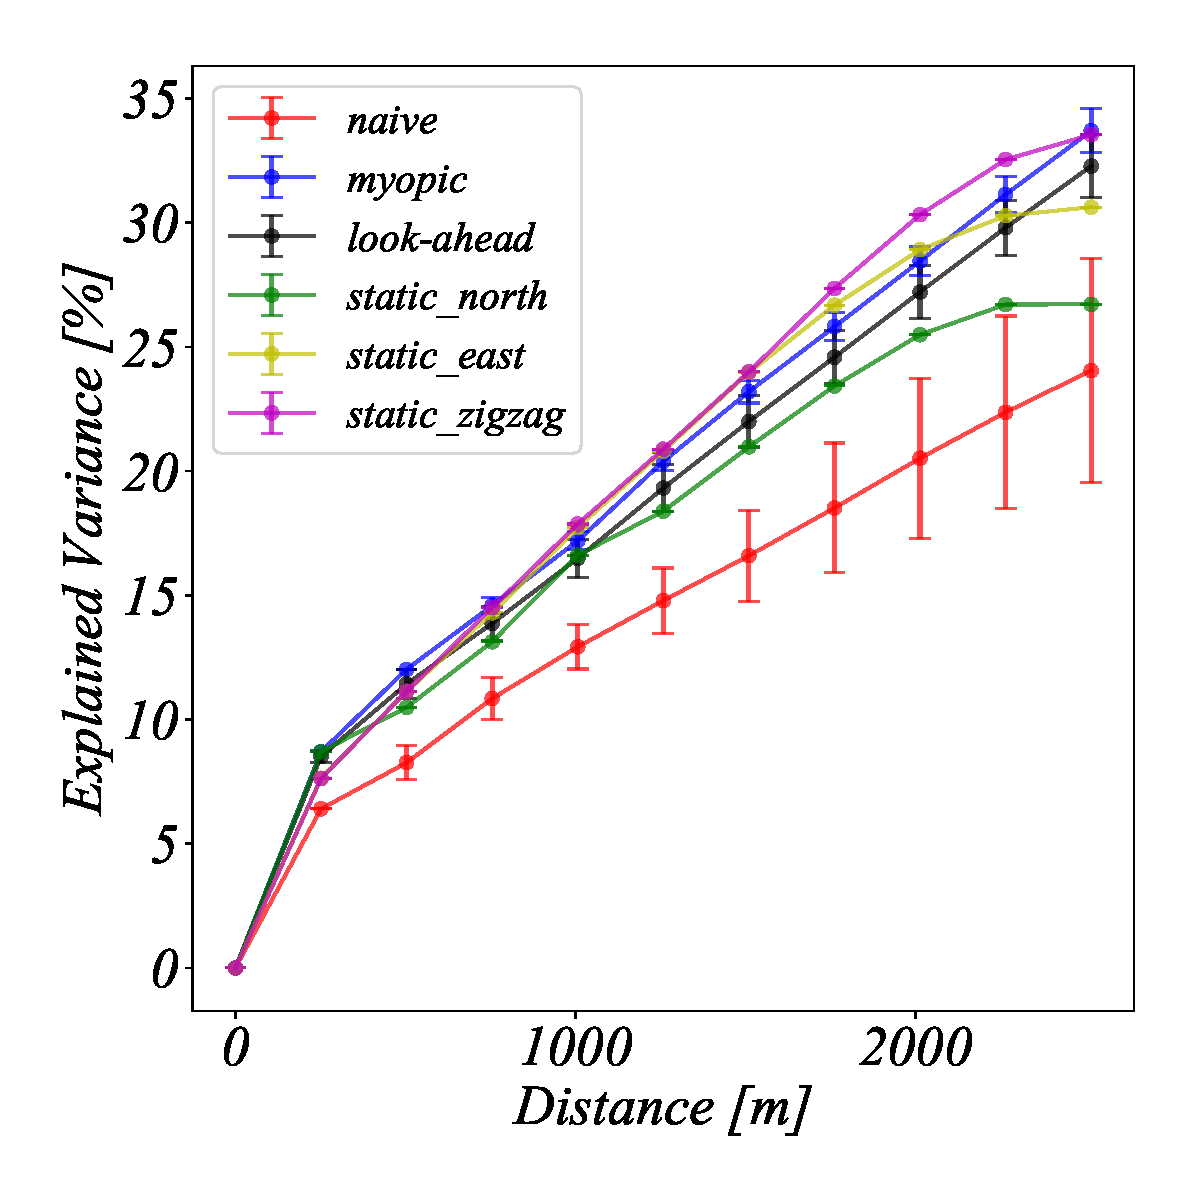
\includegraphics[height=0.49\textwidth]{Figures/sim/avg_R2.pdf}}
  \hfill 
  \subfigure[Computational time for inferencing.\kc{I see only 
    lines associated with 4 variables showing in the graph. Where is
    static\_north and static\_east?}]{\label{fig:avg_time}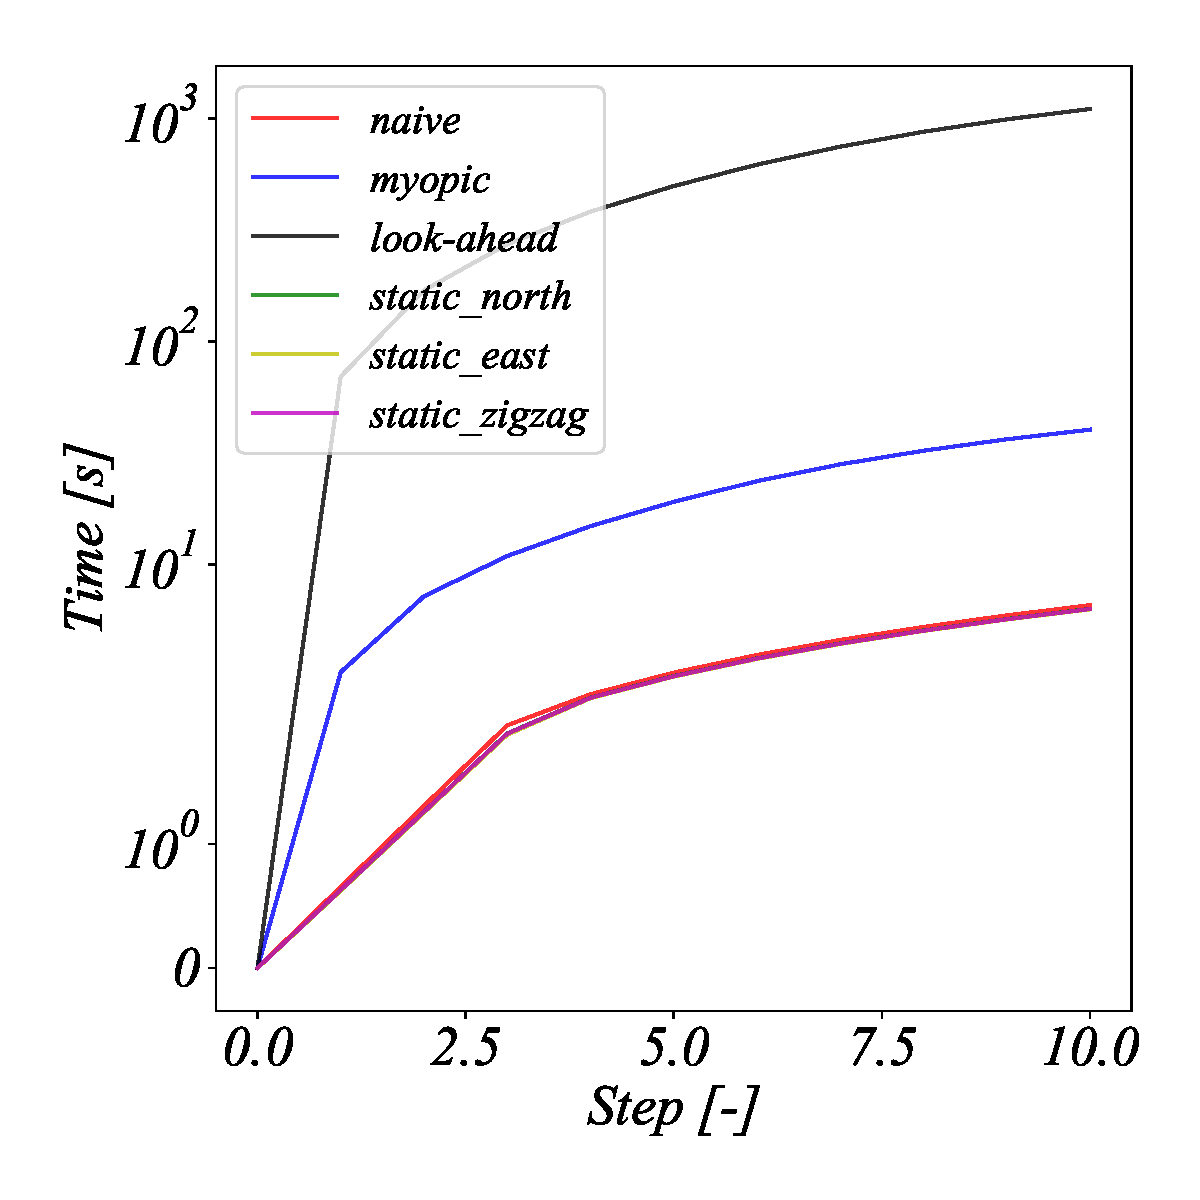
\includegraphics[height=0.49\textwidth]{Figures/sim/avg_Time.pdf}} 
\caption{Simulation results from 100 replicate simulations for 10
  sampling choices/stages on the grid. \kc{Vertical lines show large
    variation in replicate results.}}  
\label{fig:sim_results}
\end{figure}

Fig. \ref{fig:avg_rmse} and \ref{fig:avg_r2} show the resulting drop
in RMSE and increase in explained variance, respectively. Both
\textit{myopic} and \textit{look-ahead} strategies perform well here,
but some of the \textit{static\_east} and \textit{static\_zigzag} also
achieve good results because they are pre-determined to cover large
parts of the domain without re-visitation. Sequential strategies
targeting IBV will sometimes not reach similar coverage, as
interesting data may draw the path into twists and turns. There is
relatively large variety in the replicate results as indicated by the
vertical lines. Nevertheless, the ordering of strategies is similar.

\begin{figure}[!b]
  \centering
  \subfigure[Look-ahead]{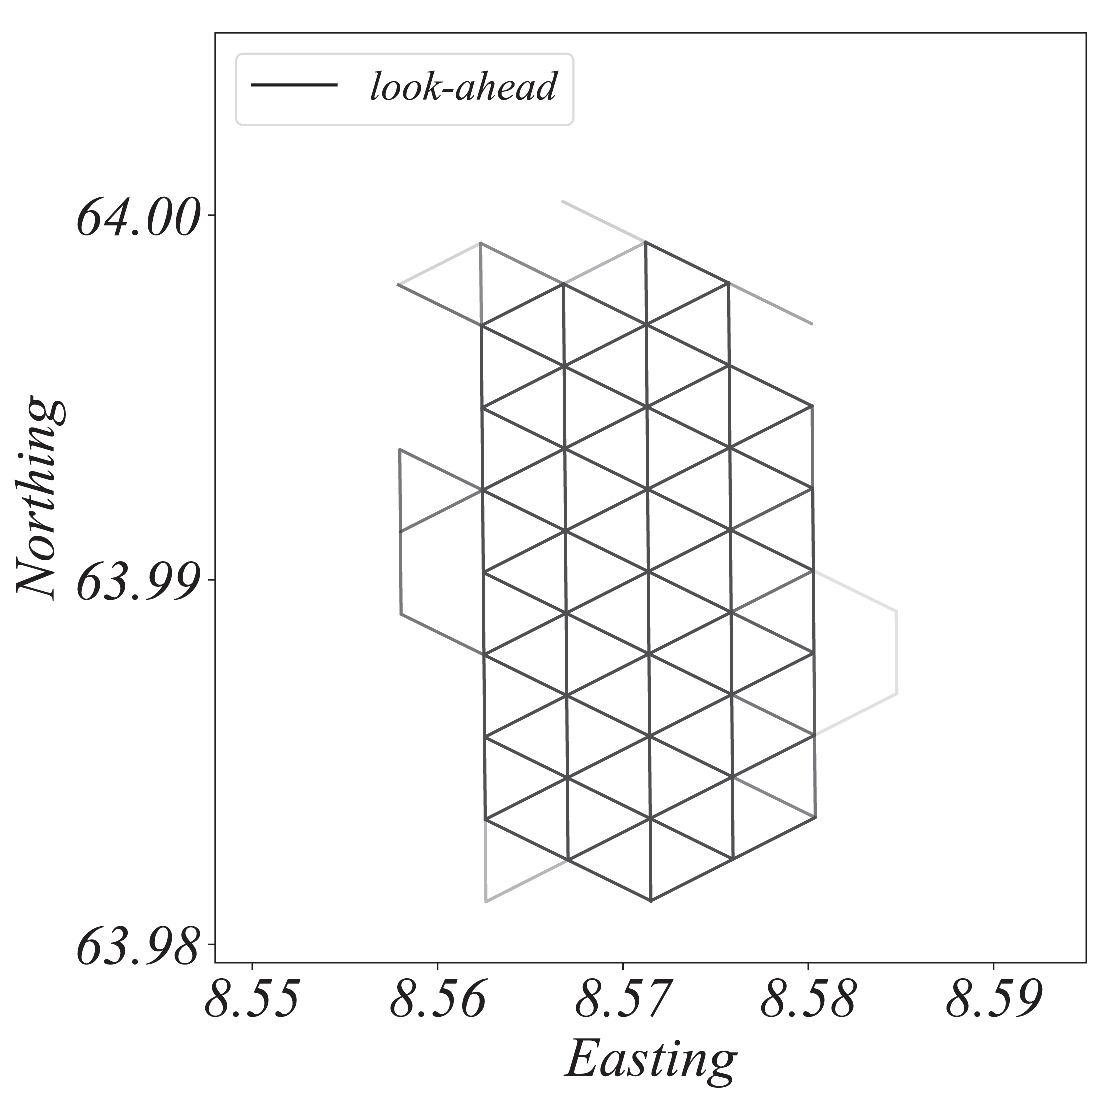
\includegraphics[height = 0.46\textwidth]{Figures/sim/route_look-ahead.pdf}\label{fig:avg_look-ahead}}
  \hfill
  \subfigure[Myopic]{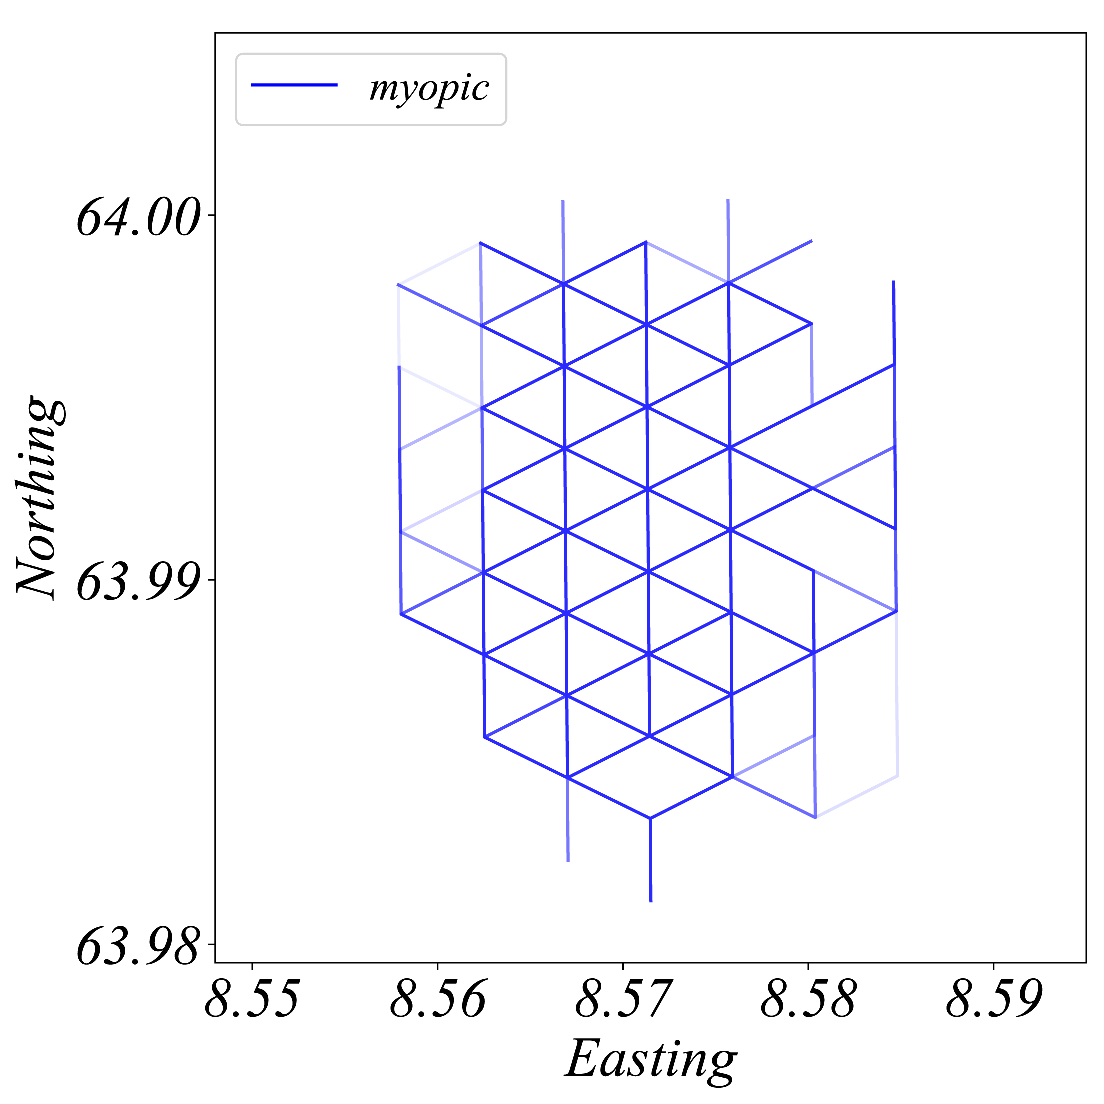
\includegraphics[height = 0.46\textwidth]{Figures/sim/route_myopic.pdf}\label{fig:avg_myopic}}
  \hfill
  \subfigure[Naive]{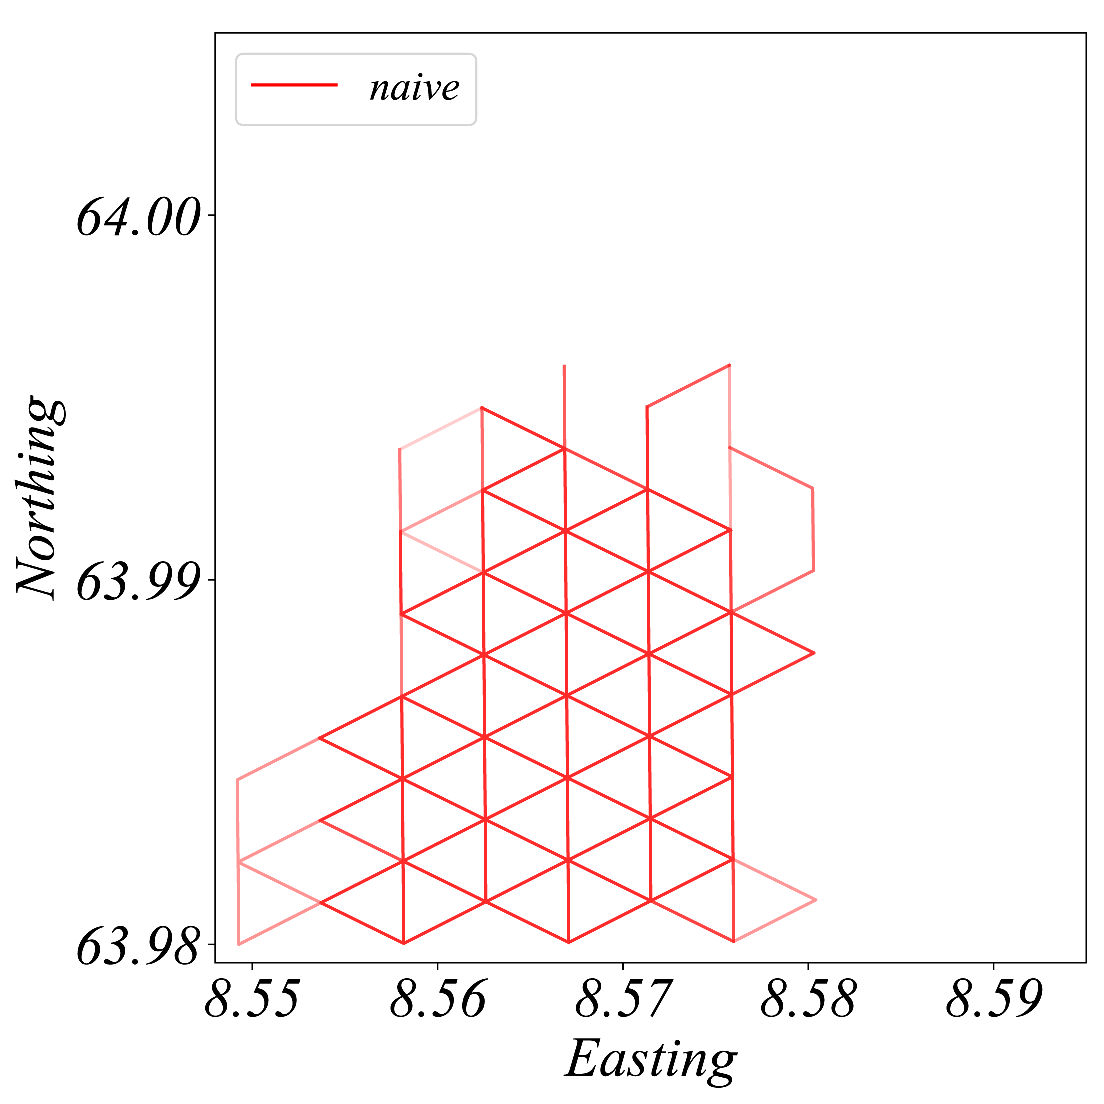
\includegraphics[height = 0.46\textwidth]{Figures/sim/route_naive.pdf}\label{fig:route_naive}}
  \hfill
  \subfigure[Static]{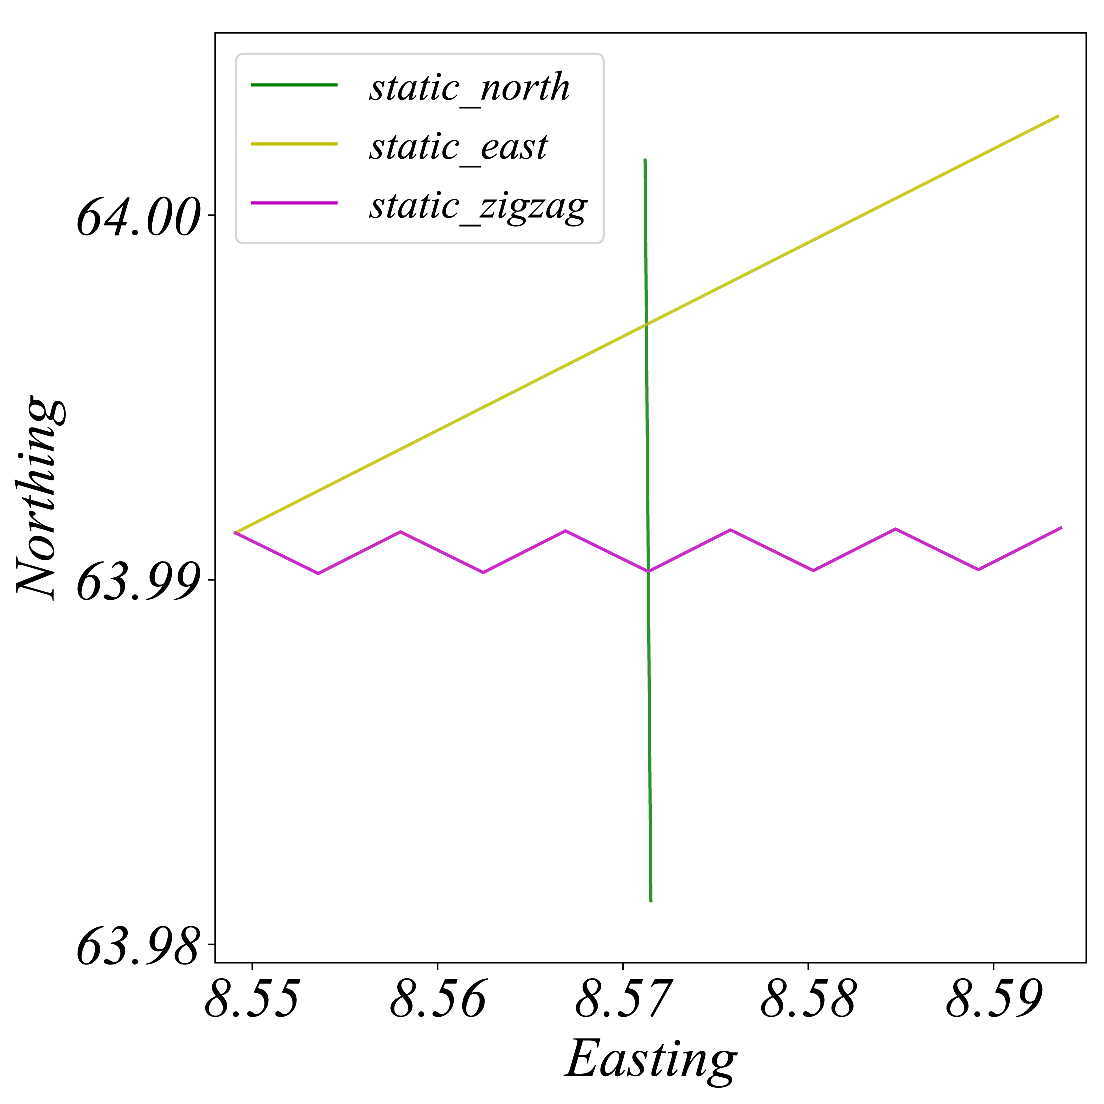
\includegraphics[height = 0.46\textwidth]{Figures/sim/route_static.pdf}\label{fig:route_static}}
  \hfill
  \caption{The overlaid route choices (strategies), superimposed on
    the 100 replicate surveys with 10 sampling choices/stages. \kc{I
      would reorder these figurs above based on the order the material
      was discussed -- Static, naive, myopic and then Look-ahead. Also
      do you really need a key associated with each subfigure, given
      the caption? An abridged analysis as in the text, might also be
      in order here in the caption. Also refer to
      Fig. \ref{fig:realisations} as the reference, where the
      temp/salinity fields are shown.}}
\label{fig:route_choices}
\end{figure}

Fig. \ref{fig:avg_time} shows the computational effort: the
\textit{naive} strategy is on par with the static designs, while the
\textit{myopic} strategy is slower. The \textit{look-ahead} is even
slower, reaching levels that are nearly impractical for execution on a
vehicle. Some pruning of the graph is performed to improve the
performance, such as ruling out repeated visitations and
back-and-forth routes. Some of the intermediate results are also
stored for longer planning horizons. Further pruning of branches or
inclusion of other heuristics could be included for better
performance. Then again, the inclusion of heuristics is likely a
contributing factor for the \textit{look-ahead} strategy failing to
outperform the \textit{myopic} strategy.

In Fig. \ref{fig:route_choices}, the realized sampling paths for each
of the sequential schemes and static designs are shown. The
\textit{naive} strategy often gets stuck in the southern part of the
domain because it is too focused on the probabilities near $0.5$. The
\textit{myopic} strategy covers a wider domain than the naive or
look-ahead. There are several reasons for this. First, a greedy
approach will tend to put more emphasis on promising locations close
to the agent, which may lead away from the centre. Second, as the
agent evaluates the impact of locations further away (look-ahead)
where assimilated data has less predictive power, the GP model (which
is centered here) will act to restrict paths deviating from the
central zone.

We studied the sensitivity of the results by modifying the input
parameters to have different correlations between temperature and
salinity, standard deviations, and spatial correlation range.  In all
runs, the \textit{myopic} and \textit{look-ahead} strategies perform
the best in terms of realized IBV, and much better than
\textit{naive}. The \textit{look-ahead} strategy seems to be
substantially better than the \textit{myopic} design only for very
small initial standard deviation or very large spatial correlation
range. \textit{static\_north} continues to be the best static design
for IBV, while \textit{static\_zigzag} is the best design for the
other predictive performance measures, especially so with large
spatial correlation range. We also ran simulation studies with only
temperature data, and for realistic correlation levels between
temperature and salinity, the IBV results are not much worse when only
temperature data are available. In addition to the comparison made in
Table \ref{tab:sim_rhoab}, the current setting includes spatial
correlation and this likely reduces the additional influence of having
bivariate data. However, it seems that having temperature data alone
does a substantially worse job in terms of explained variance

\begin{comment}
\subsection{Performance Metrics}

The tables below explore the sensitivity of the result to different input correlation values between temperature and salinity measured onboard the AUV, standard deviations, and spatial
correlations (see table rows). We only compare results at the end of
each survey. The expected ES variances are shown in Table
\ref{tab:sim_res_ev}, results of RMSE are in Table
\ref{tab:sim_res_rmse}, and explained variance is in Table
\ref{tab:sim_res_r2}. In all runs, both the \textit{myopic} and
\textit{look-ahead} strategies perform the best in terms of expected
variance in the ES. The \textit{myopic} strategy
performs slightly better than the \textit{look-ahead}. Part of the
reason for this discrepancy can be traced to the act of pruning some
of the paths for the \textit{look-ahead} strategy. The \textit{static\_north} design is clearly
better than the other two static designs, the reason being that the
others do not focus on the areas where the ES is really uncertain
(centre locations are the most uncertain). By measuring temperature
alone, the expected variances in the ES are only slightly higher than
the combined temperature-salinity estimate. This occurs because the
correlation of $0.6$ means that temperature observations provide
information about salinity as well. For the other predictive measures,
\textit{myopic} and \textit{look-ahead} strategies do well, clearly
beating the \textit{naive} strategy. 

\begin{table}[!h]
    \centering
    \scalebox{0.87}{
    \begin{tabular}{lrrrrrr}
    \toprule
    Parameter: $E_{\by}(p[1-p])$ &  naive &  myopic &  look-ahead &  static\_north &  static\_east &  static\_zigzag \\
    \midrule
                    \rowcolor{Gray}
ts. cor. low: 0.2  &  29.65 &   27.08 &       \textbf{26.44} &         32.33 &        40.31 &          36.23 \\
ts. cor. high: 0.8 &  36.18 &   \textbf{28.42} &       30.30 &         32.99 &        37.18 &          36.04 \\
                    \rowcolor{Gray}
std. low: 0.1      &  18.26 &   15.79 &       \textbf{15.35} &         18.89 &        26.65 &          26.10 \\
std. high: 0.5     &  47.01 &   \textbf{41.31} &       43.15 &         47.92 &        52.63 &          49.71 \\
                    \rowcolor{Gray}
cor. low: 0.8      &  44.42 &   \textbf{42.02} &       42.47 &         43.84 &        46.05 &          47.82 \\
cor. high: 0.2     &  29.73 &   21.09 &       \textbf{20.43} &         27.91 &        37.60 &          34.35 \\
                    \rowcolor{Gray}
temp. only         &  38.25 &   29.16 &       \textbf{28.69} &         34.32 &        39.81 &          36.17 \\
basecase           &  35.21 &   \textbf{28.56} &       28.94 &         33.50 &        39.84 &          39.26 \\
    \bottomrule
    \end{tabular}}
  \caption{Simulation results for the final mean IBV (Eq. \eqref{two_partsK}).}
    \label{tab:sim_res_ev}
\end{table}
\vspace{-0.4cm}
\begin{table}[!h]
    \centering
    \scalebox{0.92}{
        \begin{tabular}{lrrrrrr}
        \toprule
        Parameter: RMSE &  naive &  myopic &  look-ahead &  static\_north &  static\_east &  static\_zigzag \\
        \midrule
                \rowcolor{Gray}
ts. cor. low: 0.2  &   0.63 &    \textbf{0.57} &        0.59 &          0.62 &         0.57 &           0.59 \\
ts. cor. high: 0.8 &   0.63 &    \textbf{0.59} &        0.61 &          0.64 &         0.60 &           0.60 \\
                \rowcolor{Gray}
std. low: 0.1      &   0.39 &    0.37 &        0.38 &          0.38 &         0.40 &           \textbf{0.35} \\
std. high: 0.5     &   0.85 &    0.82 &        0.84 &          0.82 &         0.83 &           \textbf{0.81} \\  
                \rowcolor{Gray}
cor. low: 0.8      &   0.68 &    0.66 &        0.67 &          0.68 &         0.66 &           \textbf{0.65} \\
cor. high: 0.2     &   0.58 &    0.54 &        0.55 &          0.58 &         0.54 &           \textbf{0.49} \\
                \rowcolor{Gray}
temp. only         &   0.65 &    0.63 &        0.62 &          0.65 &         \textbf{0.61} &           0.62 \\
basecase           &  0.61 &   \textbf{0.56} &       \textbf{0.56} &         0.60 &        0.57 &          0.57 \\
        \bottomrule
        \end{tabular}}
      \caption{Simulation results for the final mean RMSE ($\frac{1}{B} \sum_{b=1}^{B} \sqrt{(\bmu-\tilde{\bmu})^2}$).}
    \label{tab:sim_res_rmse}
\end{table}
\vspace{-0.4cm}
\begin{table}[!h]
    \centering
    \scalebox{0.95}{
        \begin{tabular}{lrrrrrr}
        \toprule
        Parameter: $\bR^{2}$ &  naive &  myopic &  look-ahead &  static\_north &  static\_east &  static\_zigzag \\
        \midrule
                        \rowcolor{Gray}
ts. cor. low: 0.2  &  27.00 &   33.29 &       32.24 &         26.71 &        30.56 &          \textbf{33.50} \\
ts. cor. high: 0.8 &  23.68 &   \textbf{33.87} &       32.42 &         26.72 &        30.73 &          33.61 \\
                        \rowcolor{Gray}
std. low: 0.1      &  25.38 &   30.80 &       30.29 &         26.09 &        28.75 &          \textbf{31.66} \\
std. high: 0.5     &  26.11 &   34.22 &       32.48 &         26.95 &        31.77 &          \textbf{34.48} \\
                        \rowcolor{Gray}
cor. low: 0.8      &   8.80 &   11.50 &       11.23 &          9.56 &        12.31 &          \textbf{12.58} \\
cor. high: 0.2     &  37.57 &   \textbf{48.68} &       48.11 &         39.61 &        41.98 &          48.04 \\
                        \rowcolor{Gray}
temp. only         &  11.67 &   \textbf{22.82} &       21.98 &         18.16 &        20.77 &          22.78 \\
basecase           &  24.71 &   33.45 &       32.25 &         26.71 &        30.62 &          \textbf{33.54}\\
        \bottomrule
        \end{tabular}}
      \caption{Simulation results for the final mean explained variance $\bR^{2}=100*(1-(\Sigma_{posterior}/\Sigma_{initial}))$).}
    \label{tab:sim_res_r2}
\end{table}

\end{comment}

\section{Case Study - Mapping a River Plume}
\label{sec:case_study}

To demonstrate the applicability of using multivariate EPs and the IBV
to inform oceanographic sampling, we present a case study mapping a
river plume with an AUV. The experiment was performed in Trondheim,
Norway, surveying the Nidelva river (Fig. \ref{fig:nidelven}). The
experiments were conducted in late Spring 2019, when there is still
snow melting in the surrounding mountains so that the river water is
substantially colder than the water in the fjord. The experiment was
focused along the frontal zone that runs more or less parallel to the
eastern shore as noted in Fig. \ref{fig:nidelven}.

\subsection{Model Specification}
\label{sec:exp_modeling}

The statistical model parameters were specified based on a short
preliminary survey where the AUV made an initial transect to determine
the trends in environmental conditions and correlation
structures. Based on the initial data, the trend parameters were
estimated by linear regression, where both temperature and salinity
are assumed to increase linearly, going west from the river
mouth. Next, the residuals from the regression analysis were analyzed
to study the fit of the GP model and to specify the covariance
parameters.

%\begin{figure}[!h] 
% \centering 
%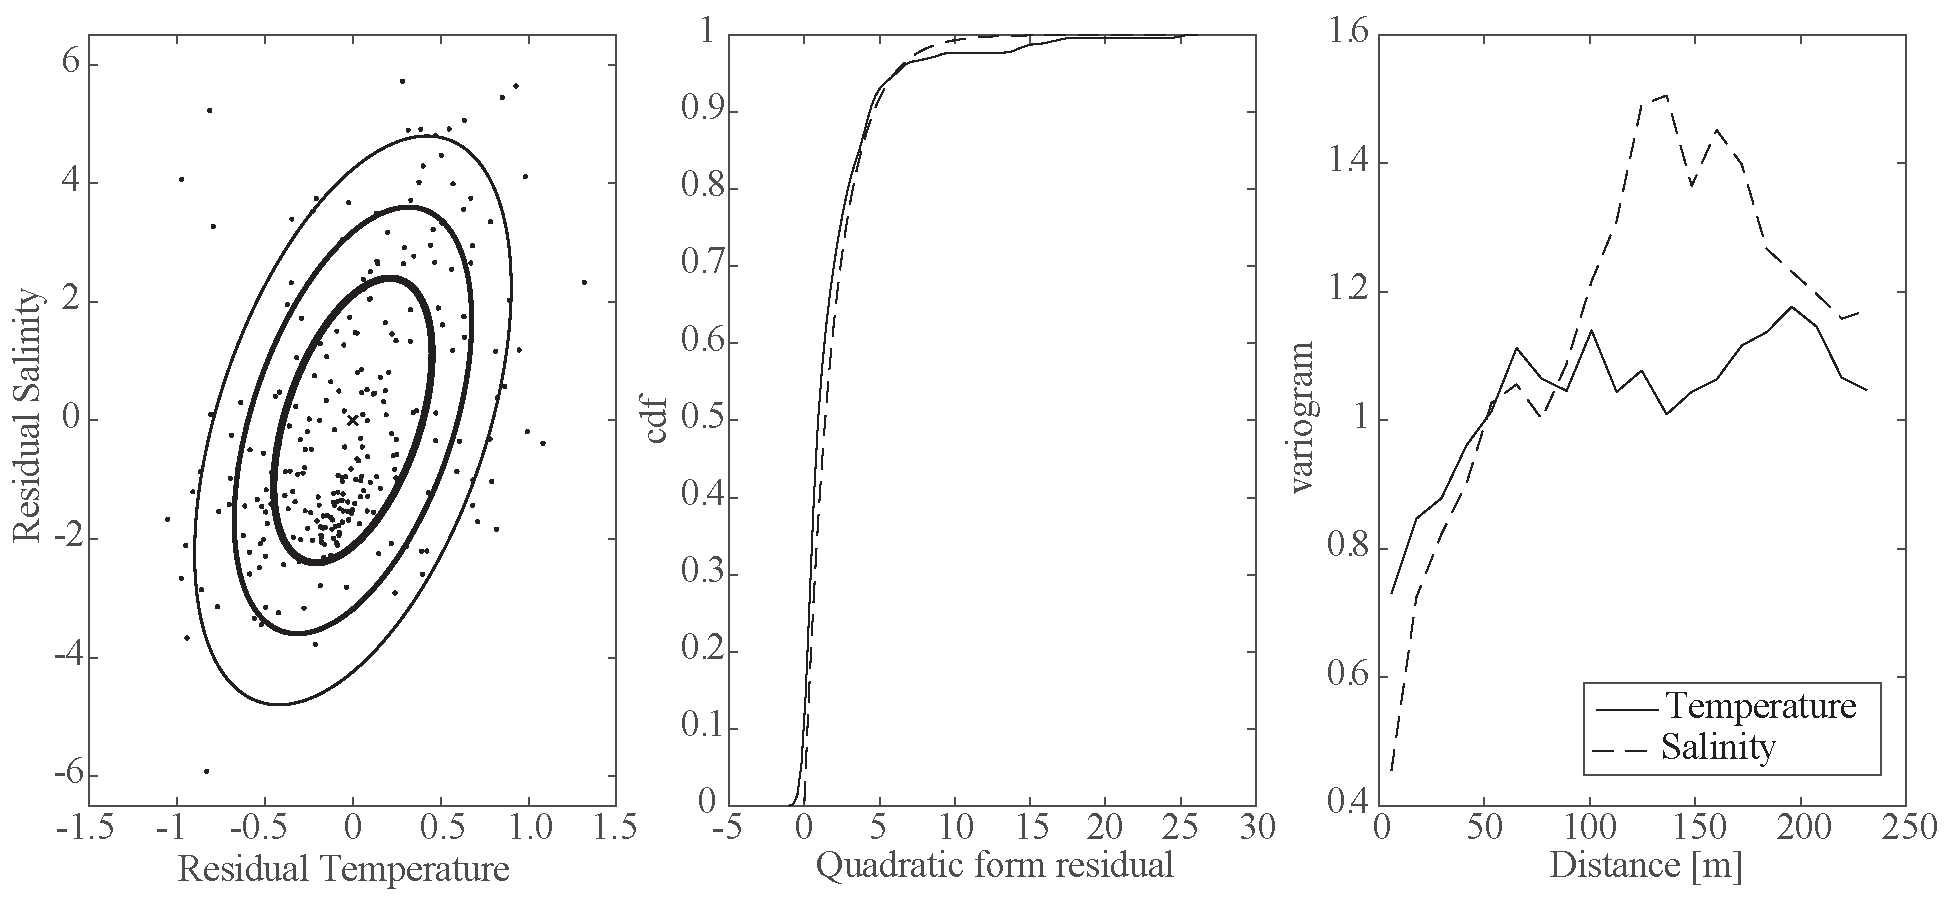
\includegraphics[width=0.98\textwidth]{Figures/field-trials/res_diag.pdf}
%\caption{Data analysis from a preliminary trial experiment using the
%  AUV. Left: Residual plot of temperature and salinity along with
%  Gaussian contours. Middle: Empirical CDF (solid) of the quadratic form of
%  the residuals along with the theoretical CDF (dashed) of the $\chi^2$
%  distribution with two degrees of freedom. Right: Empirical variogram
%  of the salinity and temperature data.} \label{fig:parest}
%\end{figure}

\begin{figure}[!h]
  \centering
  \subfigure[Residual plot.]{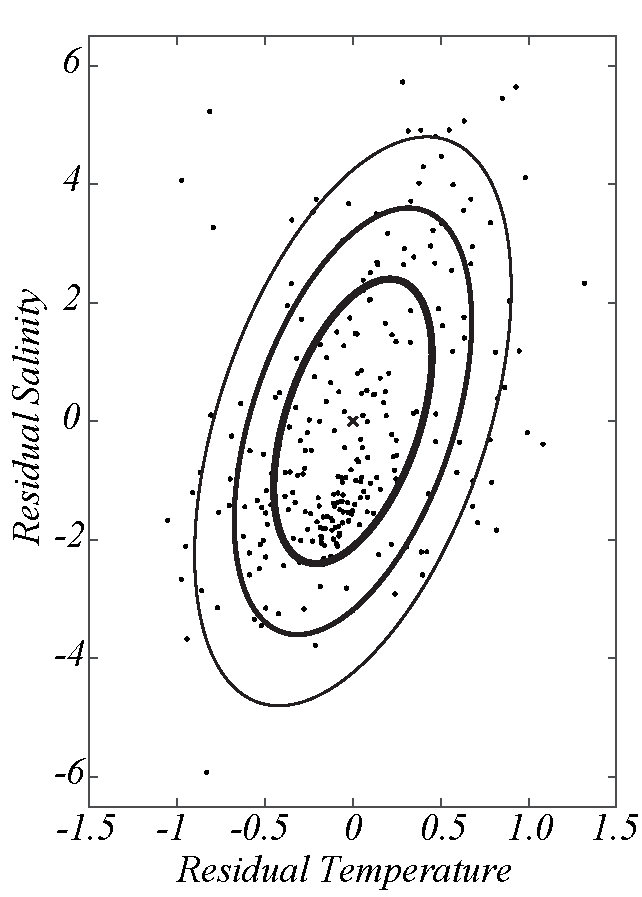
\includegraphics[width = 0.32\textwidth]{Figures/field-trials/res_diag_a.pdf}\label{fig:parest_a}}
  \hfill
  \subfigure[Empirical CDF.]{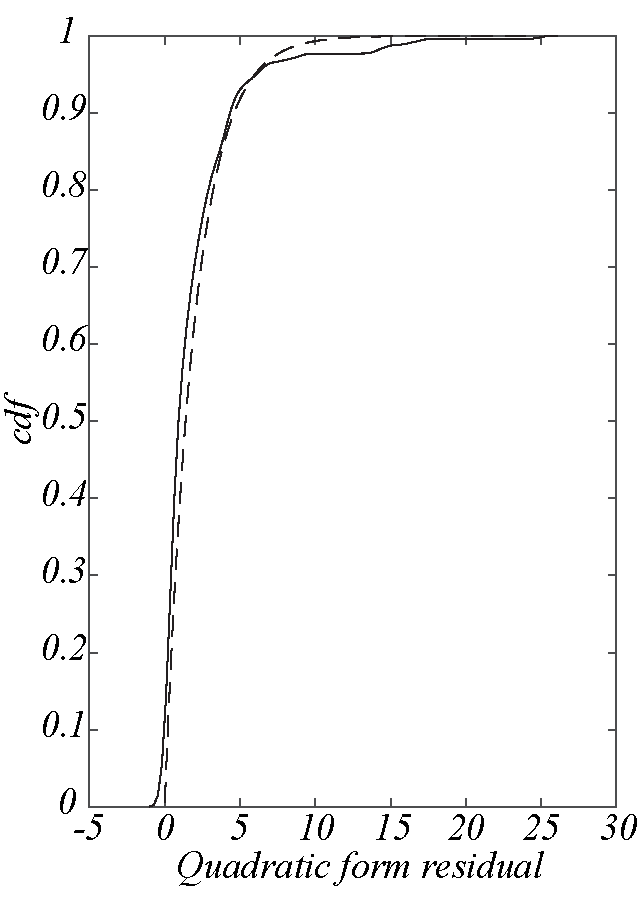
\includegraphics[width = 0.32\textwidth]{Figures/field-trials/res_diag_b.pdf}\label{fig:parest_b}}
  \hfill
  \subfigure[Empirical variogram.]{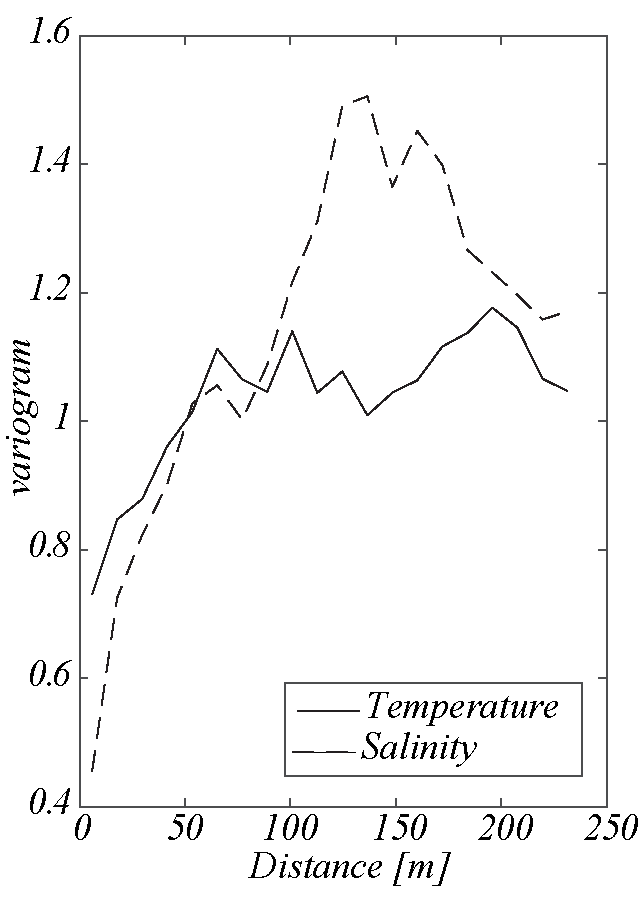
\includegraphics[width = 0.32\textwidth]{Figures/field-trials/res_diag_c.pdf}\label{fig:parest_c}}
  \caption{Data analysis from a preliminary trial experiment using the
    AUV. \ref{fig:parest_a} Residual plot of temperature and salinity
    along with Gaussian contours. \ref{fig:parest_b} Empirical CDF
    (solid) of the quadratic form of the residuals along with the
    theoretical CDF (dashed) of the $\chi^2$ distribution with two
    degrees of freedom. \ref{fig:parest_c} Empirical variogram of the
    salinity and temperature data.}
\label{fig:parest}
\end{figure}

Fig. \ref{fig:parest} summarizes diagnostic plots of this
analysis. Fig. \ref{fig:parest_a} shows a cross-plot of temperature
and salinity residuals after the westerly trends in both salinity and
temperature are subtracted from the data. This scatter-plot of joint
residuals indicates larger variability in salinity than in
temperature, and a positive correlation ($0.5$) between the two
variables. Based on the fitted bivariate Gaussian model (ellipses in
Fig. \ref{fig:parest_a}), we can compute the modeled quadratic form of
the residuals, and if the model is adequate they should be
approximately $\chi^2_2$ distributed. Fig. \ref{fig:parest_b} shows
the empirical cumulative distribution function (CDF) of these
quadratic forms (solid) together with the theoretical CDF of the
$\chi^2_2$ distribution. The modeled and theoretical curves are very
similar, which indicates that the Gaussian model fits reasonably
well. Even though there appears to be some clustering in both
Fig. \ref{fig:parest_a} and \ref{fig:parest_b}, the bivariate
diagnostic plots look reasonable and justify a Gaussian
model. Fig. \ref{fig:parest_c} shows the empirical variogram of the
scaled residuals for temperature and salinity. The decay is similar
for the two, and seems to be negligible after about $150$ m.


Based on the analysis in Fig. \ref{fig:parest}, the resulting
parameters are given in Table \ref{tab:experiment_param}. The
regression parameters shown here are scaled to represent the east and
west boundaries of the domain as seen in the preliminary transect
data, and the thresholds are intermediate values. These parameter
values were then used in field trials where we explored the
algorithm's ability to characterize the river plume front separating
the river and fjord water masses, providing a spatial map of this
boundary.

%Mapping the spatial extent of a frontal zones is an important problem for studying many bio-physical interactions in the ocean. The frontal zone is determined by the boundary where plumes of sediments, nutrients, and possibly pollutants spreading from the river outlet meet and interact with adjacent coastal water. Due to the lower density the plumes spread on the surface, creating a front with an sharp gradient in both temperature and salinity. 

\begin{table}[!h]
\centering
\begin{tabular}{lrr}
\toprule
Parameter & Value & Source\\
\midrule
\rowcolor{Gray}
Cross correlation temp. and sal. & 0.5 & AUV observations\\
Temp. variance &  0.20 & AUV observations (variogram)\\
\rowcolor{Gray}
Sal. variance &  5.76 & AUV observations (variogram)\\
Corr. range  & 0.15 km & AUV observations (variogram)\\
\rowcolor{Gray}
River temp. $T_{river}$ & $10.0\,^{\circ}\mathrm{C}$ & AUV observations\\
Ocean temp. $T_{ocean}$ & $11.0\,^{\circ}\mathrm{C}$ & AUV observations\\
\rowcolor{Gray}
River sal. $S_{river}$ & $14.0$ g/kg & AUV observations\\
Ocean sal. $S_{ocean}$ & $22.0$ g/kg & AUV observations\\
\rowcolor{Gray}
Threshold temp. & $10.5\,^{\circ}\mathrm{C}$ & $(T_{ocean}-T_{river})/2+T_{river}$\\
Threshold sal. & $18.0$ g/kg & $(S_{ocean}-S_{river})/2+S_{river}$\\
\rowcolor{Gray}
\bottomrule
\end{tabular}
\caption{Model and threshold parameters from an initial AUV
  survey. Observations were taken across the front while crossing from
  fresh, cold river water to saline and warmer ocean waters. \kc{Might
  be good to expand the terms and not have abbreviations in the table
  above; there's plenty of space.}}
\label{tab:experiment_param}
\end{table}


\subsection{Experimental Setup}

The sampling locations were distributed over an equilateral grid, as
shown in the grey-colored lattice in Fig. \ref{fig:map}. The robotic
platform consisted of a Light AUV \citep{sousa2012lauv}
(Fig. \ref{fig:lauv}) equipped with a 16 Hz Seabird Fastcat-49
conductivity, temperature, and depth (CTD) sensor providing
temperature and salinity
measurements. %The accuracy of the CTD instrument is $\pm 0.0003$ S/m (conductivity) and $\pm0.002\,^{\circ}\mathrm{C}$ (temperature).
The sampling agent was built on top of the autonomous agent framework
Teleo-Reactive EXecutive (\textit{T-REX})
\citep{py10,Rajan12,Rajan12b}, running an instance of the
\textit{myopic} strategy from Section \ref{sec:myopic} to control the
AUV and decide between sampling locations.

\begin{figure}[!h] 
\centering 

\includegraphics[width=0.98\textwidth]{Figures/harald.jpg}
\caption{The commercially available Light Autonomous Underwater
  Vehicle (LAUV) platform for upper water-column exploration used in
  our experiments.}
\label{fig:lauv}
\end{figure} 

The sampling strategy was designed around the concept of visiting
waypoints sequentially. Arriving at a desired waypoint with new
measurements and an updated model, the AUV triggers the myopic
strategy to evaluate the different design criteria (see
Eq. \eqref{critSEQ}). The waypoint-and-path combination that is
expected to reduce the IBV the most is selected, and upon arrival this
procedure is then repeated. At each stage, it takes the AUV about 30
seconds to evaluate the EIBV for all the possible waypoint-and-path
alternatives.

The AUV was set to start in the south-center part of the waypoint
graph, with the previously outlined GP model of the environment
(Section \ref{sec:exp_modeling}). A survey was set to take
approximately 40 minutes, visiting 15 waypoints on the grid, with the
AUV running near the surface to capture the plume. On its path from
one waypoint to the next, the AUV gathered data regularly, and the GP
model assimilated temperature and salinity data with an update
frequency of 30 seconds, giving about three updates per stage.

\begin{figure*}[!h]
\centering
\subfigure[AUV survey area]{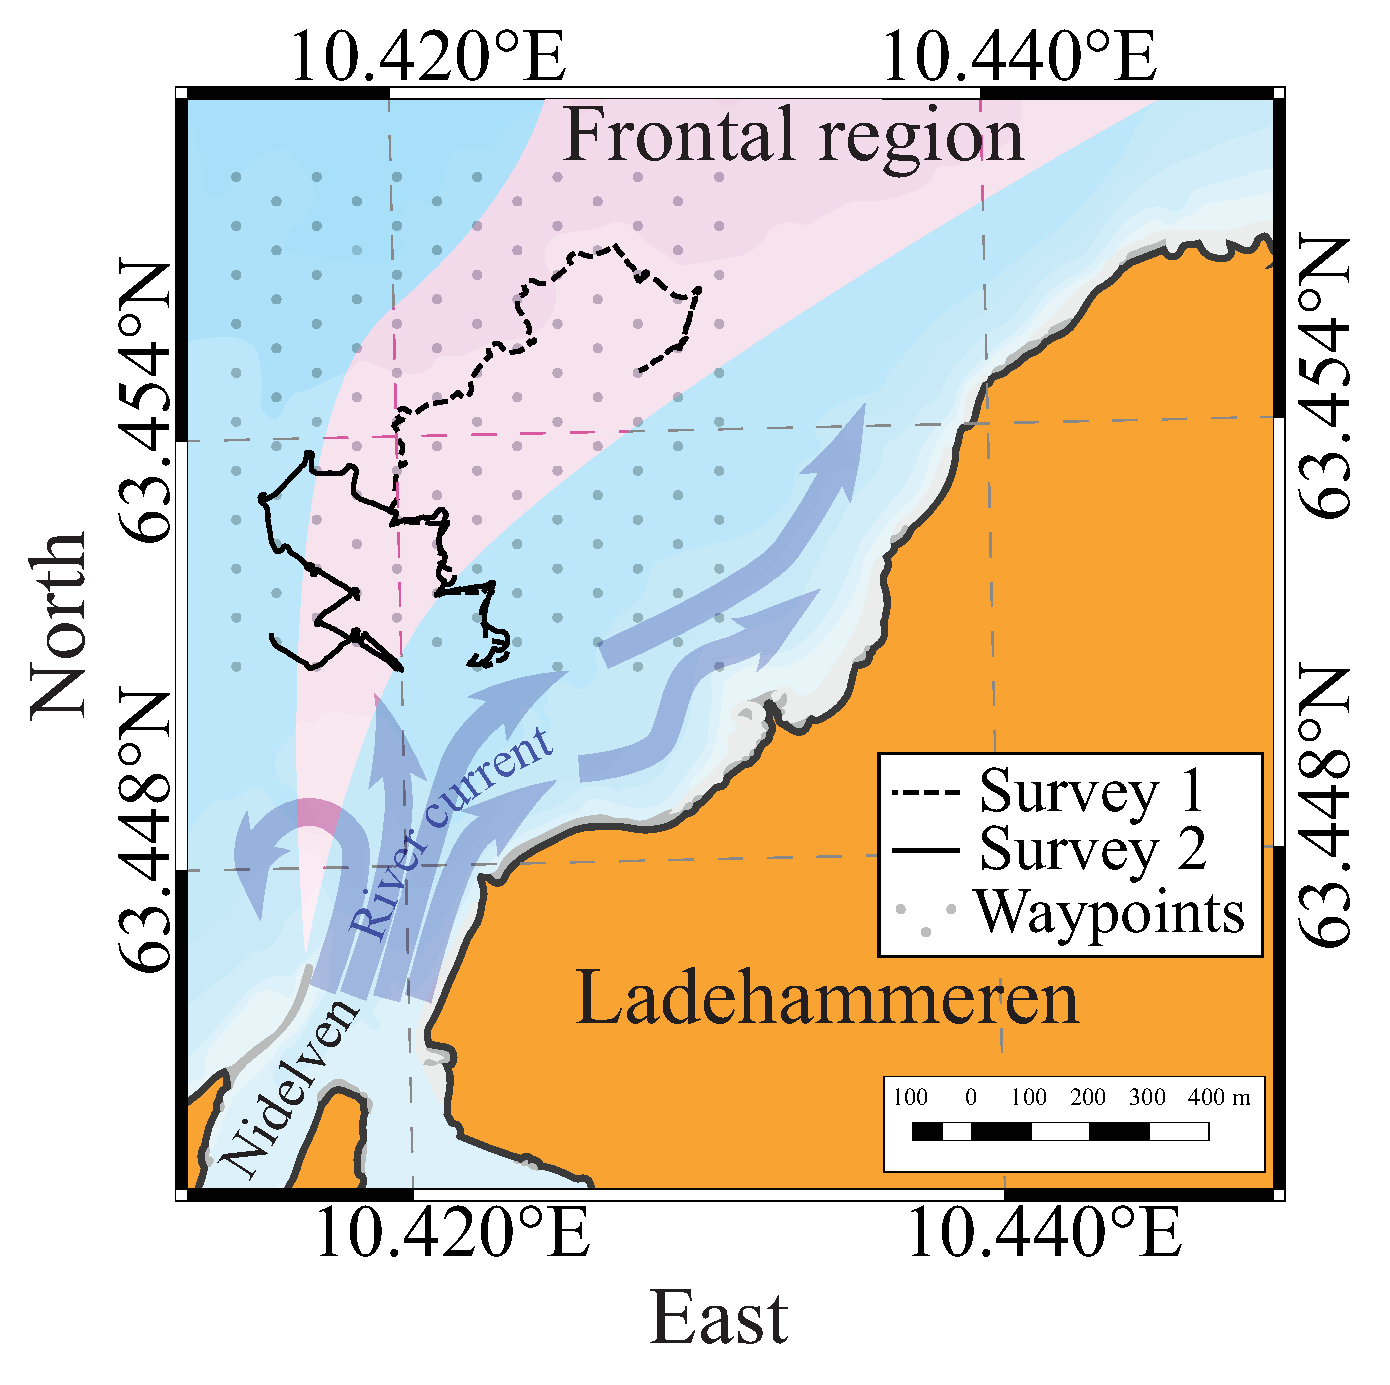
\includegraphics[height=0.41\textwidth]{Figures/field-trials/alt_map.eps}\label{fig:map}}
\hspace{0.3cm}
\subfigure[Temperature tracks]{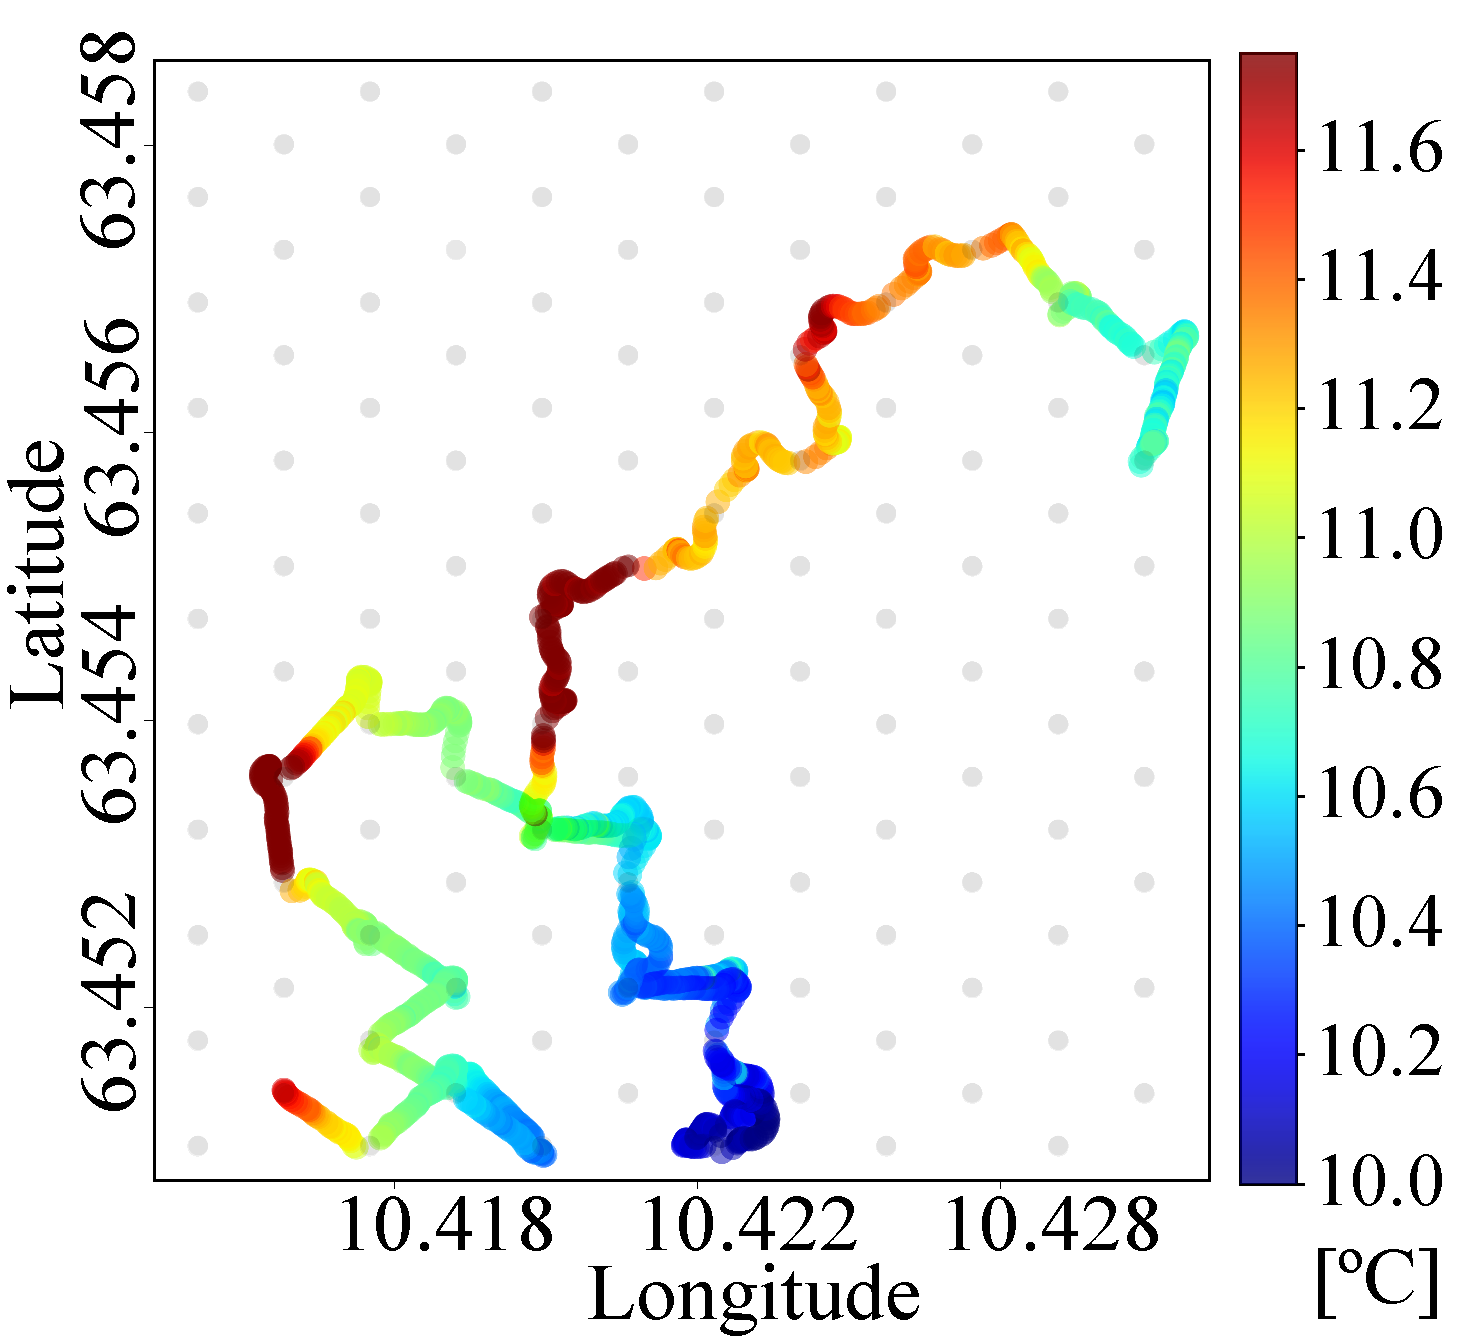
\includegraphics[height=0.41\textwidth]{Figures/field-trials/auv.pdf}\label{fig:res_both}}

\subfigure[Survey 1]{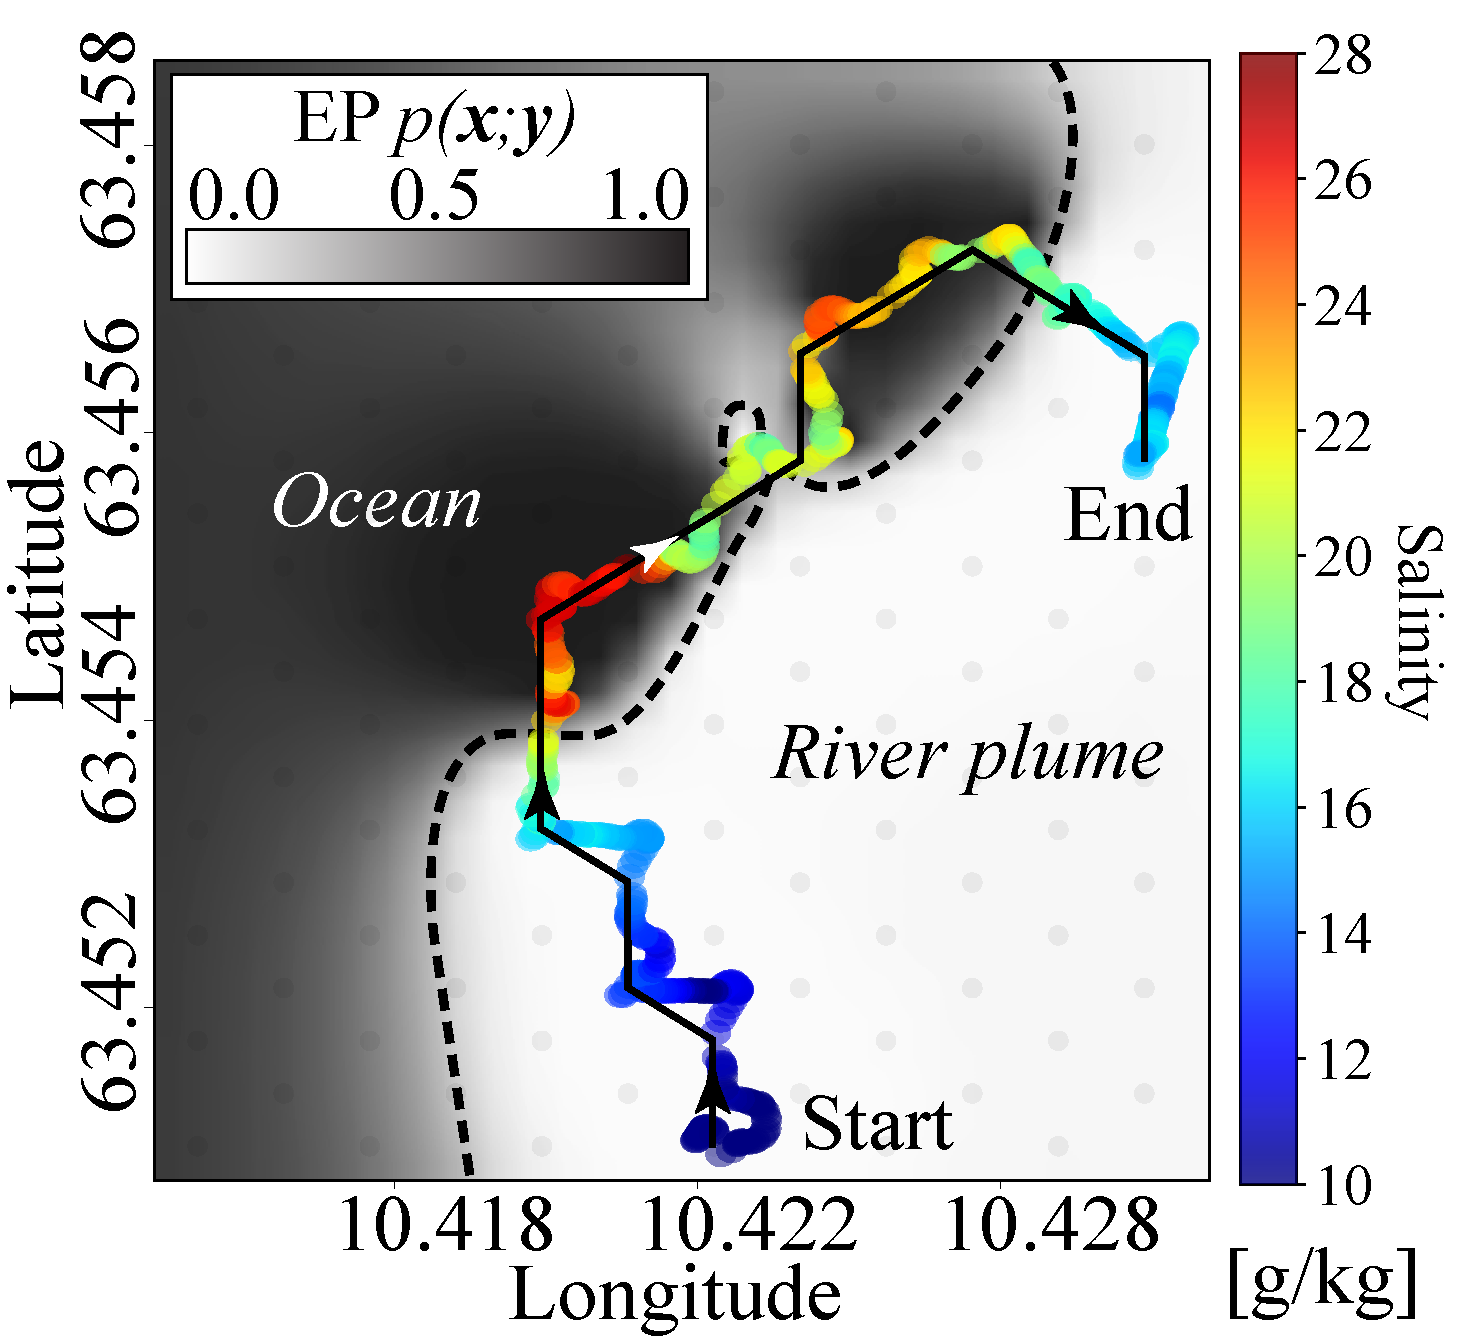
\includegraphics[height=0.40\textwidth]{Figures/field-trials/auv1_es_sal_ep.pdf}\label{fig:res1}}
\hspace{0.2cm}
\subfigure[Survey 2]{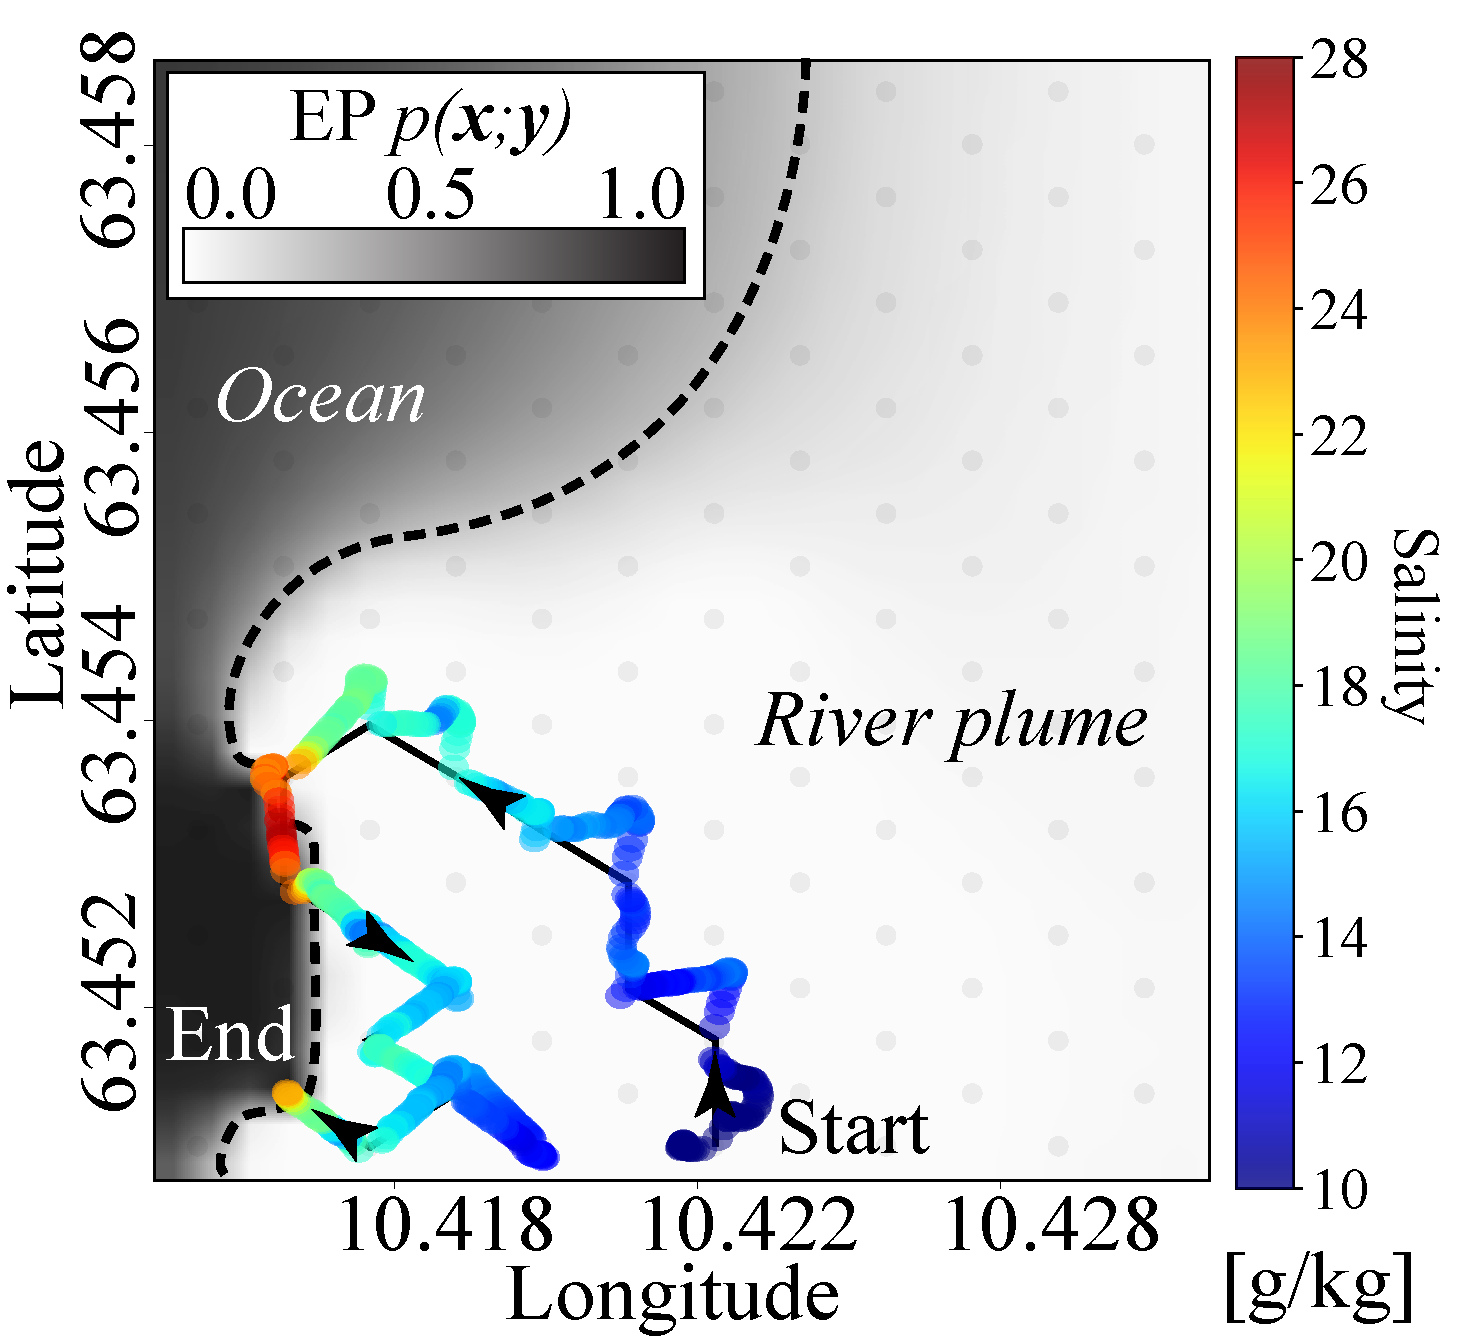
\includegraphics[height=0.40\textwidth]{Figures/field-trials/auv4_es_sal_ep.pdf}\label{fig:res2}}

%\subfigure[ES for Survey 1]{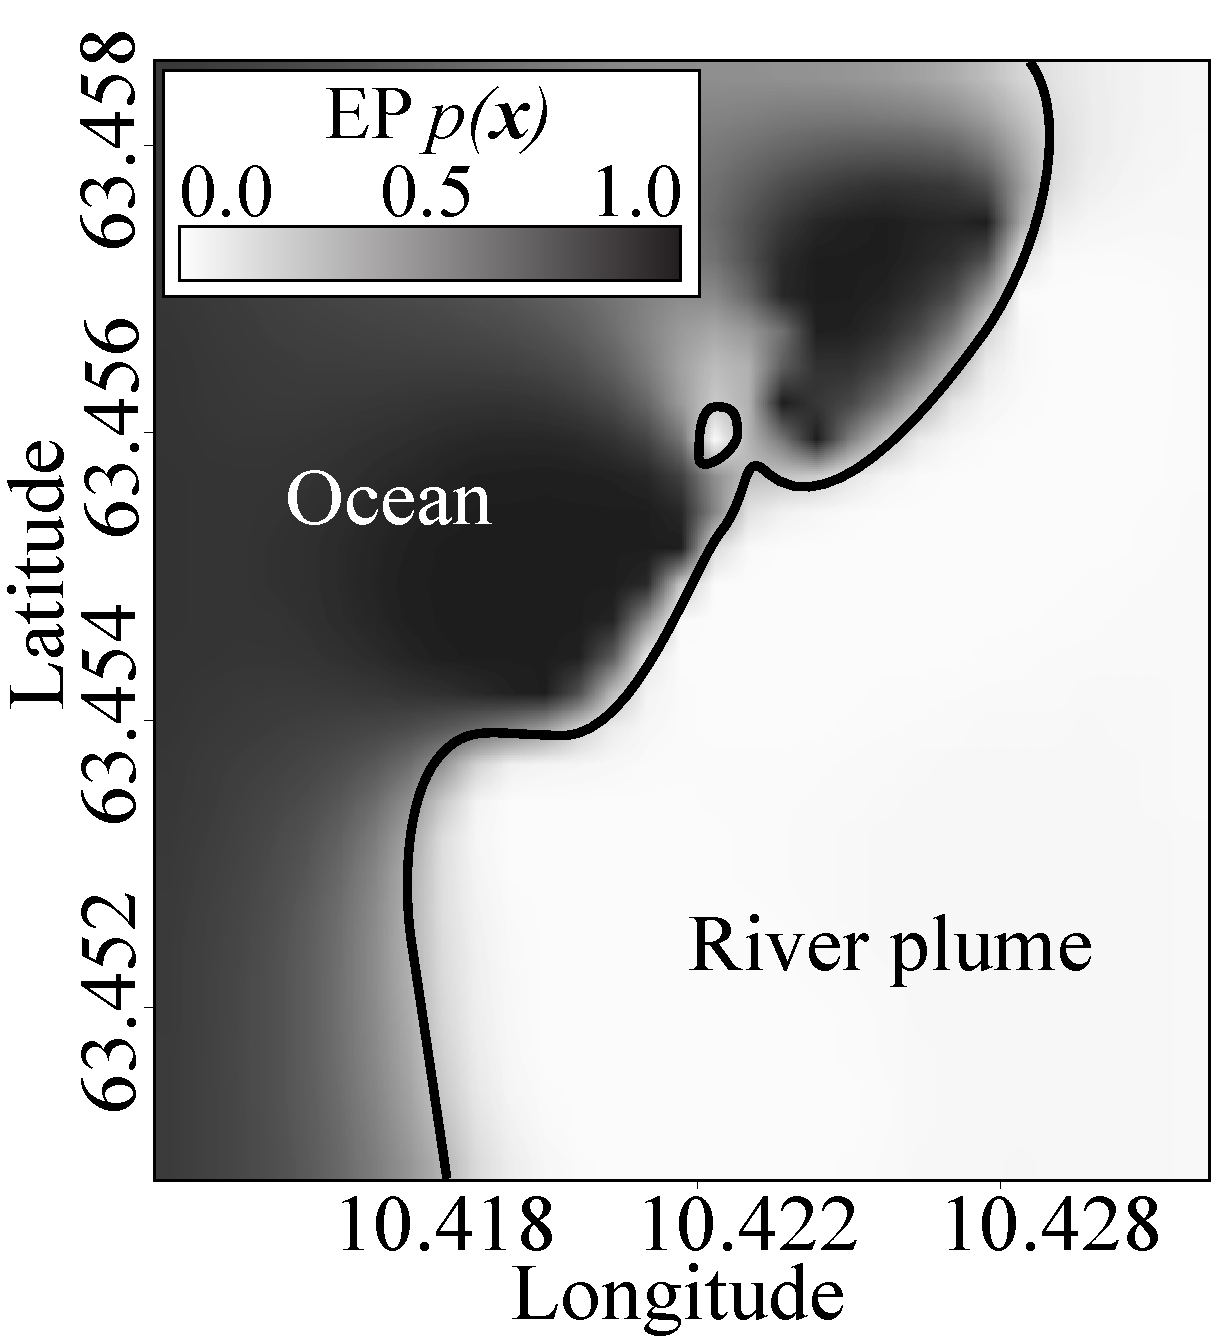
\includegraphics[height=0.41\textwidth]{Figures/field-trials/ep_1.pdf}\label{fig:res3}}\hspace{0.4cm}
%\subfigure[ES for Survey 2]{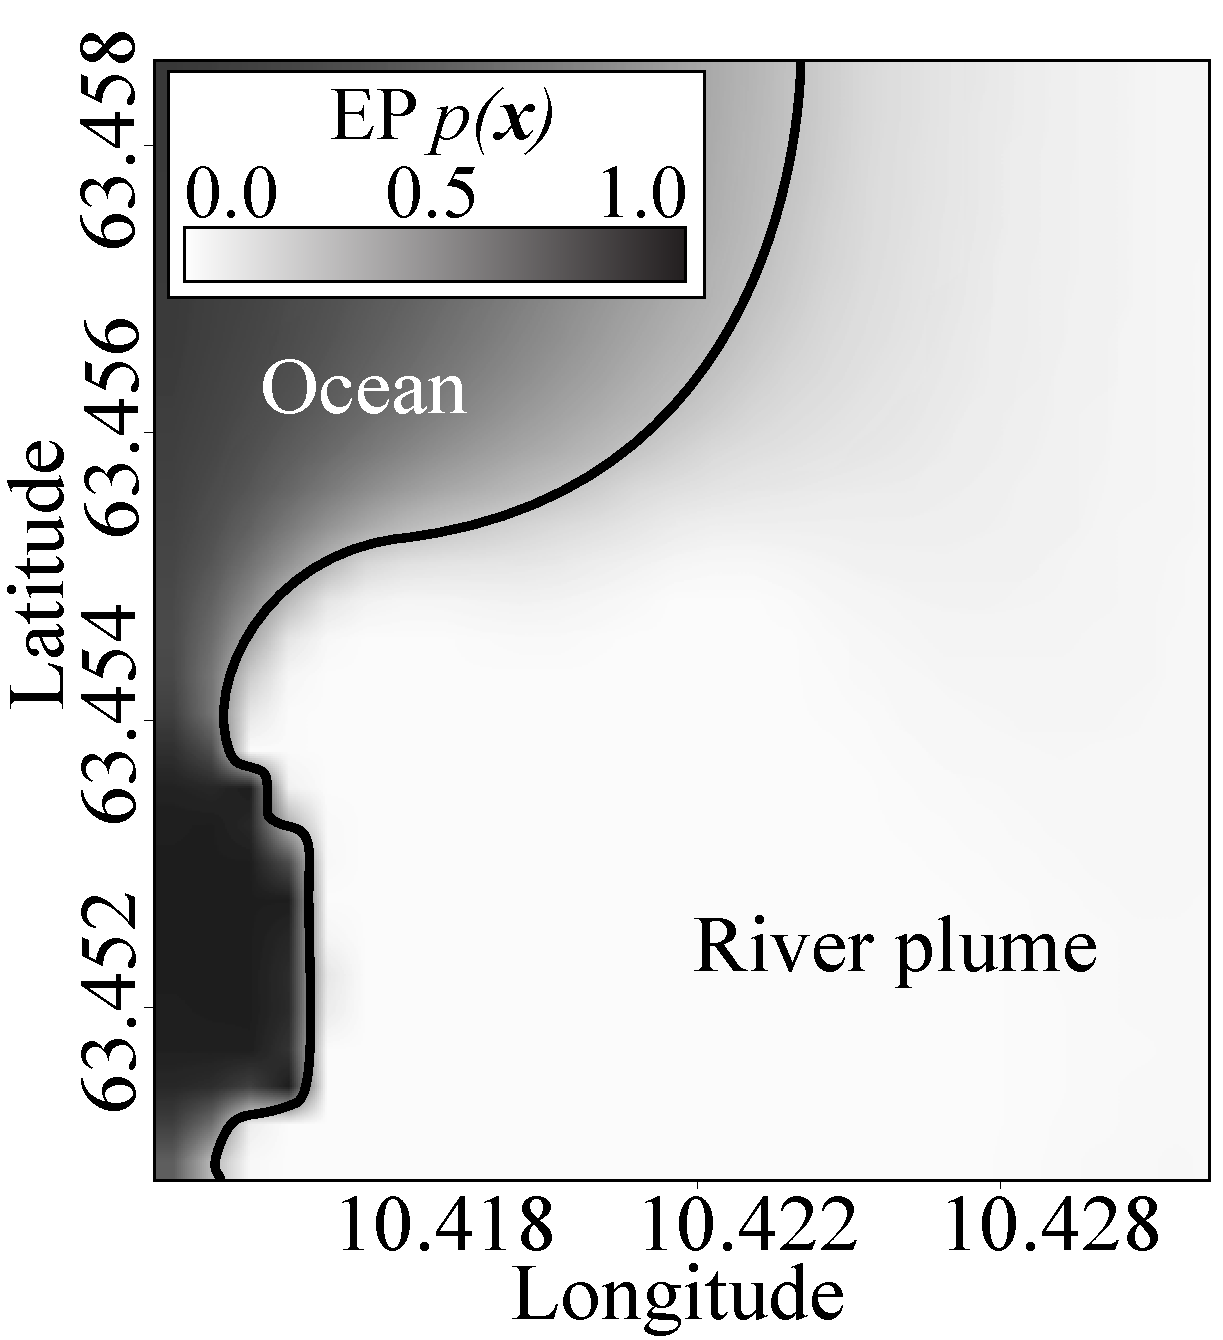
\includegraphics[height=0.41\textwidth]{Figures/field-trials/ep_4.pdf}\label{fig:res4}}
\caption{Results from mapping the Nidelva river, Trondheim, Norway
  over two survey missions. \ref{fig:map} shows an overview of the
  survey area overlaid with the AUV path in black and dashed
  line. Note the shaded region indicating a typical frontal
  region. \ref{fig:res_both} shows the collected temperature data as
  colored trails. Note waypoint 5 (WP5) which indicates where the two
  surveys diverge. \ref{fig:res1} and \ref{fig:res2} shows the
  collected salinity data overlaid on the final EP, which indicate the
  AUVs statistical impression of the front. For both missions the
  temperature and salinity data correspond with an indication of the
  EP front. \kc{Might want to indicate when the surveys (dates) were
    conducted so people can understand the variability in the EP with
    respect to time.}}
\label{fig:results}
\end{figure*}

\subsection{Results}

Two surveys missions (1 and 2), were run successively from 11:00 AM to
01:00 PM, with a short break in between. The resulting path of the
selected waypoints are shown in the map in Fig. \ref{fig:map}, both
within the expected frontal region (shaded pink). The recorded
temperatures are shown as colored trails in Fig. \ref{fig:res_both},
clearly indicating the temperature difference between fjord and
riverine waters. The salinity data are then shown separately, overlaid
with the estimated EP for each survey in Fig. \ref{fig:res1} and
\ref{fig:res2}.

Both surveys successfully estimated and navigated the separation zone,
crossing the frontal boundary multiple times. As conditions changed
slightly between the two surveys, the resulting path (after waypoint
5) is shown to deviate. Survey 1 continued northwards, tracking the
north-eastern portion of the front, while Survey 2 turned west,
mapping the south-western region.

The final predictions of the front location, represented by
conditional EPs in Fig. \ref{fig:res1} and \ref{fig:res2} as dashed
lines, correspond with one another. In both surveys they yield a
picture of the front being to the west in the southern portions of the
region and gradually bending off toward the north east. The amount of
exploration done by Survey 1 is greater than Survey 2. In Survey 1,
the AUV obtained more detail by going north from waypoint 5, while
Survey 2, coming close to the survey area borders in the south-western
corner, obtained a poorer understanding of the northern parts. A
look-ahead strategy might identify and discourage such choices.

%\begin{figure}[!h] 
% \centering 
%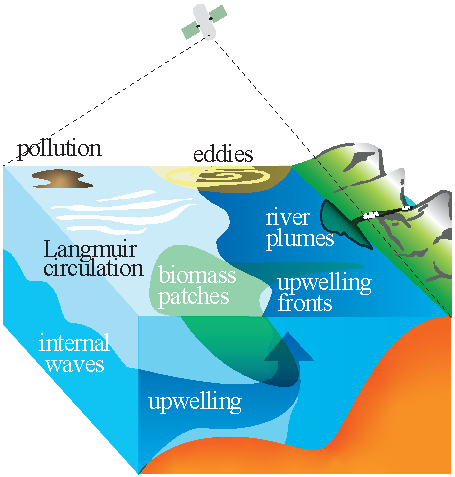
\includegraphics[width=0.48\textwidth]{Figures/envir_ocean.pdf}
%\caption{Ocean observation is moving away from %single-ship sampling
%towards more collaborative networked operations in %order to resolve
%the numerous processes and their interaction.} %\label{fig:envir}
%\end{figure}
%\newpage
\section{Closing remarks}\label{sec:concl_disc}

This work builds on a multidisciplinary effort combining statistical
modeling with robotic surveying techniques for oceanographic
applications. We show how observation practices can gain efficiency
and accuracy from the development of statistical techniques to achieve
more effective spatial monitoring. We further demonstrate the
opportunities available for real-time multivariable spatial
data-gathering and analysis onboard autonomous platforms, which
statisticians can exploit to create general-purpose toolkits for
similar applications.

In particular, we derive and show results for characterizing phenomena
connected to the properties of water masses. The characterization of
uncertainties in random sets is extended with new results for the EIBV
uncertainty reduction achieved by spatial sampling design. This is
provided in closed-form for the situation with a static design, and
then extended to the adaptive situation. The sequential derivations
provide new insights into efficient applications of adaptive sampling,
as demonstrated in our application.

The study did not consider any temporal effects, which would be
relevant on a larger time scale. We consider the extension to
spatio-temporal modeling as future work, and envision that
advection-diffusion equations could be useful in this kind of modeling
\citep{sigrist2015stochastic}. For more complex oceanographic
phenomena, the methods will need to be extended to non-Gaussian
phenomena, possibly feature-based mixtures of GPs which could still be
run onboard and augmented by dynamical models. \kc{How about talking
  about removing any grids or waypoints altogether?}

The spatial-statistical design criterion, building on random sets is
relevant in our setting with different water properties, and we show
mathematical generality beyond the EIBV which is convenient to
implement for onboard robotic planning. Such criteria could also be
useful in other oceanographic settings as for algal-blooms, anoxic
zones or open water fronts \cite{costa19}. Of course, other criteria
are also relevant for instance, hybrid or multi-attribute criteria
that could balance goals of exploration and exploitation in this
situation. Equally, such techniques have significant use cases in
downstream decision-making, with policy makers and regulators who need
to make difficult decisions related to fish farming, other marine
resource operations. Value of information analysis (VOI)
\citep{Eidsvik:15} could be used in a similar vein as the IBV in the
current work, as both analytic methods explore when, where and which
information is likely to result in improved decision-making.

While more effort could be spent on approximating the look-ahead
stages in the adaptive designs, it is perhaps more interesting to
explore the additional flexibility that can be gained by having
multiple AUVs co-temporally exploring a spatial or spatio-temporal
domain \citep{ferreira2019advancing}. Such an approach would enable
concurrent sampling in different parts of the space, or opportunities
to move in parallel to best capture the excursion set.

\section*{Acknowledgements}

TOF acknowledges support from the Centre for Autonomous Marine
Operations and Systems
(AMOS)\footnote{\url{https://www.ntnu.edu/amos}}, Center of
Excellence, project number 223254, and the Applied Underwater Robotics
Labortatory (AURLab). JE and KR acknowledge support from Norwegian
research council (RCN), project number 305445. CT and DG acknowledge
support from the Swiss National Science Foundation, project number
178858.

%\begin{supplement}
%\sname{Supplement A}\label{suppA}
%\stitle{Title of the Supplement A}
%\slink[url]{http://www.e-publications.org/ims/support/dowload/imsart-ims.zip}
%\sdescription{Dum esset rex in
%accubitu suo, nardus mea dedit odorem suavitatis. Quoniam confortavit
%seras portarum tuarum, benedixit filiis tuis in te. Qui posuit fines tuos}
%\end{supplement}

% == Adding references
\footnotesize
\bibliographystyle{imsart-nameyear}
\bibliography{ref}


\section*{Appendix}


Proof of Proposition \ref{propo1}:

\begin{proof}
	That $\mes(\es)$ defines indeed a random variable follows from Fubini's theorem 
	relying on the joint measurability of 
	$(\x, \omega) \to \mathbbm{1}_{\es(\omega)}(\x)$, 
	%= \mathbf{1}_{\xi_{\x}(\omega) \in T}$ and Fubini's theorem.  
	itself inherited from the assumed measurability for  
	$(\x, \omega) \to \gp[\x](\omega)$ and $T$, respectively. From there, following the steps of Robbins' theorem \cite{Robins1944}, we find that 
	\begin{equation*}
	\begin{split}
	\mathbb{E}[\mes(\es)^{r}]
	&=\mathbb{E}\left[\left(\int_{D} \mathbbm{1}_{\gp[u] \in T} ~d\mes(u) \right)^{r} \right]
	=\mathbb{E}\left[ \prod_{i=1}^{r} \left(
	\int_{D} \mathbbm{1}_{\gp[\uu^{(i)}] \in T} ~d\mes(\uu^{(i)}) 
	\right) \right] \\
	&
	=
	%\mathbb{E}\left[
	%\int_{D^{r}}
	%\prod_{i=1}^{r}
	%\mathbf{1}_{\gp[\uu^{(i)}] \in T}
	%\productMeasure
	%\right]
	%=
	\mathbb{E}\left[
	\int_{D^{r}}
	\mathbbm{1}_{\gp[\uu^{(1)}] \in T,\dots, \gp[\uu^{(r)}]  \in T}
	\productMeasure
	\right]
	%\\
	%&=\int_{D^{r}} \mathbb{E}\left[\mathbf{1}_{\gp[\bm{u}] \in T^r} \right] \productMeasure \\
	%&
	=\int_{D^{r}}
	\jointExcuProb 
	\productMeasure.
	\end{split}
	\end{equation*}   
	The rest consists in expliciting the probability of $T\times \dots \times T$ under the multivariate Gaussian distribution of  
	$\left(\gp[u^{(1)}], \dots,  \gp[u^{(r)}] \right)$. 
\end{proof}

Proof of Proposition \ref{propo2}:

\begin{proof}
	By definition of $\Phi_{p}$, for $N\sim \mathcal{N}_{p}(0_{p},\covN)$, 
	$$
	\mathbb{P}(N\leq a + BV | V)
	=
	\varPhi_{p}\left( a + BV; \covN \right).
	$$
	Now for $\varPhi_{p}\left( a + BV; \covN \right)^h$, provided that the probability space is sufficiently large to accomodate $h$ independent Gaussian random vectors $N_i\sim \mathcal{N}_{p}(0,\covN)$ (which is silently assumed here), using the former equality delivers 
	$$
	\varPhi_{p}\left( a + BV; \covN \right)^h
	=
	\prod_{i=1}^h \mathbb{P}(N_i\leq a + BV | V).
	$$
	Now by independence of the $N_i$'s we obtain the joint conditional probability 
	$$
	\prod_{i=1}^h \mathbb{P}(N_i\leq a + BV | V)
	=
	\mathbb{P}(N_1\leq a + BV, \dots, N_h\leq a + BV| V),
	$$
	whereof, by virtue of the law of total expectation, 
	\begin{equation*}
	\begin{split}
	\mathbb{E}\left[ \varPhi_{p}\left( a + BV; \covN \right)^h \right]
	&=\mathbb{E}\left[\mathbb{P}(N_1\leq a + BV, \dots, N_h\leq a + BV| V)\right]\\
	&=\mathbb{P}(N_1\leq a + BV, \dots, N_h\leq a + BV)\\
	&=\mathbb{P}(W_1 \leq a, \dots, W_h\leq a)\\
	&=\varPhi_{ph}
	\left(
	1_{h} \otimes a
	;
	(1_{h}1_{h}')\otimes (B\Sigma_{V} B') + 
	I_{h}\otimes \covN
	\right),
	\end{split}
	\end{equation*}
	where $\mathbf{W}=(W_1,\dots,W_h)$ with $W_i=N_i- BV \ (1\leq i \leq h)$
	and the last line follows $\mathbf{W}$ forming a Gaussian vector (by global independence of the $N_i$'s and $V$) and from the definition of $\varPhi_{p h}$. The covariance matrix $\mathbf{\Sigma}$ of $\mathbf{W}$ is obtained by noting that $\operatorname{cov}(W_i,W_j)=B \covV B' + \delta_{ij} \covN \ 
	(i,j \in \{1,\dots,h\})$.
	%the latter concatenated Gaussian vector is obtained by straightfoward calculation. 
\end{proof}


Proof of Proposition \ref{propo3}.

\begin{remark}
	%    Note that the vector $\bm{a}$ is obtained by stacking $h_i$ times each $a_i$
	%\begin{equation*}
	%\bm{a} = \begin{pmatrix}
	%    \bm{a}_1\\ \vdots\\ \bm{a}_g\end{pmatrix},~
	%\bm{a}_i =
	%\begin{pmatrix}
	%    a_i\\ \vdots\\ a_i\end{pmatrix}
	%\in\mathbb{R}^{l\times h_i}\end{equation*}
	%and the covariance matrix is obtained by similar stacking
	Using blockwise representation for the blocks themselves delivers %$\bm{\Sigma}$ can be expressed as follows
	\begin{equation*}
	%    \bm{\Sigma} = \begin{pmatrix}
	%        \Sigma_{11} & & \Sigma_{1g}\\
	%        & \ddots &\\
	%        \Sigma_{g1}&   & \Sigma_{gg}
	%\end{pmatrix},~
	\Sigma_{ij} =
	\begin{pmatrix}
	B_i\Sigma_{V} B_j' & \dots & B_i\Sigma_{V} B_j'\\
	\vdots & & \vdots\\
	B_i\Sigma_{V} B_j' & \dots & B_i\Sigma_{V} B_j'\\
	\end{pmatrix}
	+
	\delta_{ij}
	\begin{pmatrix}
	\covN_i & &\\
	& \ddots &\\
	&   & \covN_i
	\end{pmatrix}%\in\mathbb{R}^{lh_i\times lh_j}
	\end{equation*}
	Here each $\Sigma_{ij}$ is made of $h_i$ times $h_j$
	(vertically/horizontally) $p \times p$ sub-blocks, hence possesses $ph_i$ lines and $ph_j$ columns.
\end{remark}

%Proof TODO along with notation polish. 

\begin{proof}
	The proof relies (again) heavily on the fact that, by definition of $\Phi_{p}$, for any covariance matrix $\covN \in \R^{p \times p}$, $a\in \R^p$, $B\in \R^{p \times q}$, and $N\sim \mathcal{N}_{p}(0_{p},\covN)$, 
	$$
	\mathbb{P}(N\leq a + BV | V)
	=
	\varPhi_{p}\left( a + BV; \covN \right).
	$$
	In particular, for globally independent $N_{i,j} \sim \mathcal{N}_{p}(0_{p},\covN_i)$ $(1\leq j \leq h_i, 1\leq i \leq g)$, 
	\begin{equation*}
	\begin{split}
	\prod_{i=1}^{g} \varPhi_{p}\left(a_i + B_{i}V; \covN_{i} \right)^{h_i}
	&=
	\prod_{i=1}^{g}
	\prod_{j=1}^{h_{i}}
	\mathbb{P}(N_{i,j}\leq a_i + B_i V | V)\\
	&=\mathbb{P}(N_{1,1}\leq a_1 + B_1 V, \dots, N_{g,h_{g}}\leq a_g + B_g V | V),
	\end{split} 
	\end{equation*}
	so that, by the law of total expectation, 
	\begin{equation*}
	\begin{split}
	\mathbb{E}\left[ \prod_{i=1}^{g} \varPhi_{p}\left(a_i + B_{i}V; \covN_{i} \right)^{h_i} \right]
	=
	\mathbb{P}(W_{1} \leq 1_{h_{1}} \otimes a_1, \dots, W_{g} \leq 1_{h_{g}} \otimes a_g)
	\end{split}
	\end{equation*}
	where 
	$W_{1}=(N_{1,1}- B_1 V, \dots, N_{1,h_{1}}- B_1 V), 
	W_{2}=(N_{2,1}- B_2 V, \dots, N_{2,h_{2}}- B_2 V), 
	\dots, W_{g}=(N_{g,1}- B_g V, \dots, N_{g,h_{g}}- B_g V)$. Noting that $\mathbf{W}=(W_1,\dots, W_g)$ is a centred $p H$-dimensional Gaussian random vector, we finally obtain that 
	\begin{equation*}
	\begin{split}
	\mathbb{E}\left[ \prod_{i=1}^{g} \varPhi_{p}\left(a_i + B_{i}V; \covN_{i} \right)^{h_i} \right]
	=
	\varPhi_{p H}\left(\bm{a};\mathbf{\Sigma}\right),
	\end{split}
	\end{equation*}
	with $\bm{a}=(1_{h_{1}} \otimes a_1, \dots, 1_{h_{g}} \otimes a_g)$ and $\bm{\Sigma}=(\operatorname{cov}(W_i,W_j))_{i,j \in \{1,\dots, g\}}$.
\end{proof}


% AOS,AOAS: If there are supplements please fill:
%\begin{supplement}[id=suppA]
%  \sname{Supplement A}
%  \stitle{Title}
%  \slink[doi]{10.1214/00-AOASXXXXSUPP}
%  \sdatatype{.pdf}" 
%  \sdescription{Some text}
%\end{supplement}

% === Not used
% After reviews: - This is moved to Section 2.1. 

%Traditional data collection at sea has typically been based on static
%buoys, Lagrangian floats, or ship-based methods, with significant
%logistical limitations that directly impact coverage and sampling
%resolution. Modern methods using satellite remote-sensing provide
%large-scale coverage but have limited resolution, are limited to
%sensing the surface of the ocean, and are impacted by cloud cover. The
%advent of robust mobile robotic platforms \citep{Bellingham07} has
%resulted in significant contributions to environmental monitoring and
%sampling. In particular, autonomous underwater vehicles (AUVs), have
%advanced the state of sampling and consequently have made robotics an
%integral part of ocean observation; our previous work has contributed
%to this effort \citep{das11b,Das2015,fossum18b,fossuminformation}. Other ¤ %statistical work in the oceanographic domain include \cite{wikle2013modern}
%focusing on hierarchical statistical models; \cite{sahu2008space},
%studying spatio-temporal models for sea surface temperature and
%salinity data; and \cite{mellucci2018oceanic} looking at the
%statistical prediction of features using an underwater glider.

%\begin{itemize}
%
%\item Full numerical ocean models cannot provide accurate results
%  online if run on robotic sensing platforms, as onboard computers
%  cannot deliver the computational power required. Hence statistical
%  proxy models of the environment must be used for learning where to sample.
%
%\item With limited available information about the state of the ocean, there is substantial value in reacting to
%  information obtained from measurements taken in-situ. This
%  acquired information must be assimilated into statistical models that
%  can be used to inform decisions on where to sample
%  sequentially.%\emph{in-situ}; this is usually referred to as the \emph{adaptivity gap} \citep{ause2008phd}.
%
%\item For sampling problems related to environmental sensing, the
%  number of choices (i.e. locations, trajectories, and candidate
%  designs) is enormous, creating a
%  trade-off between optimization (finding the most resource-efficient
%  design to collect necessary data) and computability (arriving at a
%  solution in reasonable time). To successfully resolve features, this
%  trade-off has to be considered in development and practice.
%
%\end{itemize}

%Addressing this, the combination of statistical tools and robotic platforms is a
%natural symbiosis which enables information-based sensing. Central to
%this is the ability to model spatially-correlated variables and
%provide formal measures of uncertainty. Our formulation is based on
%Gaussian Processes (GPs) as they allow efficient implementation 
%and evaluation in real time onboard a robotic platform.

%Sampling can, in this context, not simply be distributed evenly ---along simple transects or ``lawn-mover" patterns--- but must instead be prioritized to relevant regions to ensure it is cost-effective while providing adequate coverage and resolution of the area of scientific interest.

%While the focus has often been on
%biological and anthropogenic impact from micro-plastics to
%pollution, biological oceanographers have focused intently on studying
%micro-organisms at the base of the human food web. These organisms are
%critically impacted by the changing dynamics in the upper water-column,
%especially in coastal zones which are complex and often hard to observe
%in space and time. By studying the bio-geochemical processes in the
%upper water-column scientists can measure the impact of change, natural
%or anthropomorphic, and provide an informed opinion to policy makers to
%effect changes in preserving the environment. However, the challenge of 
% The pressure on marine resources is growing and increased accuracy,
% resolution, and persistent monitoring of the oceans is crucial for
% long-term sustainable management. 

% A
% sustained focus on prioritized and efficient data collection strategies
% have therefore started to emerge. The advent of marine robotic
% platforms, especially

% provided means to execute this prioritization through the capacity of
% autonomy and data-driven sampling, where data collection in principle
% can be optimized. These capabilities have made

% of the emerging sensing practice for ocean science, allowing scientists
% to increase the observational efficiency and resolution beyond what was
% previously possible. But how should a robotic platform, such as an AUV,
% effectively prioritize and identify important regions for sampling? The
% answer to this question relates to 

% , and
% the application domain is clearly an arena where statisticians can
% contribute.
% There has recently been some statistical attention in oceanography:

%From an oceanographic perspective, interesting regions are usually directly tied to a distinct phenomena that is of scientific interest. Each phenomenon can in turn be characterized by a set of process specific conditions expressed through different measures of key environmental variables, such as temperature or salinity. One such measure is the gradient, that can be associated with a number of important processes, such as the vertical location of the thermocline and pycnocline, location of upwelling systems, vertical mixing, eddies, fronts, and currents \cite{sverdrup2006}, as well as distribution, growth, and accumulation of biological activity \cite{SatOceanSoci00, Ryan2014}. These gradients create boundaries separating the ocean into process specific regions which are of profound interest to both identify and map effectively. Quantification of gradient features is therefore a much needed competence in robotic sampling.
\end{document}

